%% ======================================================================
%% M.Tech. Phase I Report -- IIT Bombay
%% Compile with:  pdflatex -> bibtex -> pdflatex -> pdflatex
%% Required files: main.tex, mybib.bib, asmejour.bst, and the figure files
%% (figures may sit next to main.tex or in a sub-folder named "figures").
%% ======================================================================
\documentclass[a4paper,12pt,oneside]{report}

%================================================
% Fonts, encoding, microtypography
%================================================
% newtxtext + newtxmath: complete, uniform Times New Roman for all text and math.
% amsmath must be loaded first; amssymb is omitted as newtxmath provides those symbols.
\usepackage[T1]{fontenc}
\usepackage[utf8]{inputenc}
\usepackage{amsmath}                     % load before newtxmath to avoid conflicts
\usepackage{newtxtext}                   % Times New Roman text (body, headings, captions)
\usepackage{newtxmath}                   % Times-matched math fonts, includes AMS symbols
\usepackage{microtype}

%================================================
% Page layout
%================================================
% Margins: the original side margins (3.25 cm) are kept; top and bottom are
% made equal (3 cm) so that the text block is symmetric on the page.
\usepackage[a4paper,left=3.25cm,right=3.25cm,top=3cm,bottom=3cm]{geometry}

%================================================
% Mathematics, graphics, tables, lists
%================================================
\usepackage{graphicx}
\usepackage{subcaption}
\graphicspath{{./}{figures/}}
\usepackage{booktabs}
\usepackage{array}
\usepackage{xcolor}
\usepackage{enumitem}
\setlist{topsep=6pt,itemsep=2pt,parsep=0pt}

%================================================
% Spacing
%================================================
\usepackage{setspace}
\usepackage{etoolbox}
\setstretch{1.5}                                % main body: 1.5 line spacing
\AtBeginEnvironment{figure}{\singlespacing}     % figures, captions: single
\AtBeginEnvironment{table}{\singlespacing}      % tables, captions: single
\raggedbottom
\clubpenalty=10000
\widowpenalty=10000
\displaywidowpenalty=10000
\tolerance=1500
\emergencystretch=2em

%================================================
% Floats and captions
%================================================
\usepackage[section]{placeins}                  % floats do not drift past a \section
% font={normalfont,small}: captions use the same Times New Roman as the body.
\usepackage[font={normalfont,small},labelfont=bf,labelsep=period,skip=6pt]{caption}
\captionsetup[figure]{position=below}
\captionsetup[table]{position=above}
\usepackage{subcaption}
\renewcommand{\topfraction}{0.9}
\renewcommand{\bottomfraction}{0.8}
\renewcommand{\textfraction}{0.1}
\renewcommand{\floatpagefraction}{0.7}
\setcounter{topnumber}{3}
\setcounter{bottomnumber}{2}
\setcounter{totalnumber}{4}

%================================================
% Citations and headings
%================================================
\usepackage{cite}
\renewcommand{\bibname}{References}

\usepackage{titlesec}
\titleformat{\chapter}[display]
  {\normalfont\singlespacing\bfseries\centering}
  {\Large\chaptertitlename\ \thechapter}{10pt}{\LARGE}
\titleformat{name=\chapter,numberless}[display]
  {\normalfont\singlespacing\bfseries\centering}{}{0pt}{\LARGE}
\titlespacing*{\chapter}{0pt}{0pt}{24pt}
\titleformat{\section}
  {\normalfont\singlespacing\large\bfseries}{\thesection}{0.75em}{}
\titleformat{\subsection}
  {\normalfont\singlespacing\normalsize\bfseries}{\thesubsection}{0.75em}{}
\titlespacing*{\section}{0pt}{18pt plus 4pt minus 2pt}{8pt plus 2pt}
\titlespacing*{\subsection}{0pt}{14pt plus 3pt minus 2pt}{6pt plus 2pt}
\setcounter{tocdepth}{2}

%================================================
% Project-specific commands
%================================================
% Table helpers: uniform table font, row spacing and column spacing; wide tables
% are scaled down only if they are wider than the text (never scaled up).
\newcommand{\tablestyle}{\footnotesize\renewcommand{\arraystretch}{1.2}\setlength{\tabcolsep}{4pt}}
\newcommand{\fitwidth}[1]{\resizebox{\ifdim\width>\linewidth\linewidth\else\width\fi}{!}{#1}}
\newcolumntype{L}[1]{>{\raggedright\arraybackslash}p{#1}}

% Standard figure widths
\newcommand{\figwidth}{0.7\textwidth}
\newcommand{\figwidthwide}{0.85\textwidth}

% Hard-typed citation numbers that could not be matched to the .bib file.
% They print exactly as before; while the switch below is true they are red.
\newif\ifmarkhardcites
\markhardcitestrue
\newcommand{\hardcite}[1]{\ifmarkhardcites\textcolor{red}{[#1]}\else[#1]\fi}

% Front-matter headings (unnumbered, same look as chapter titles)
\newcommand{\frontpagebegin}[1]{\clearpage\phantomsection\addcontentsline{toc}{chapter}{#1}}
\newcommand{\frontheadingtext}[1]{\begin{center}{\normalfont\bfseries\LARGE #1}\end{center}\vspace{24pt}}
\newcommand{\frontheading}[1]{\frontpagebegin{#1}\frontheadingtext{#1}}

%================================================
% hyperref: loaded last
%================================================
\usepackage[hidelinks,bookmarksnumbered,plainpages=false,pdfusetitle,
  pdfauthor={U Rohit Krishnan}]{hyperref}
\hypersetup{pdftitle={Finite Element Trained Machine-Learned Model for Inverse Identification of Hydrogen Trap Parameters from TDS Data in Pipeline Steel}}

%================================================
% Document
%================================================
\begin{document}

\pagenumbering{roman}

%================================================
% TITLE PAGE
%================================================
\thispagestyle{empty}

\begin{singlespace}
\begin{center}

{\Large\bfseries
FINITE ELEMENT TRAINED MACHINE-LEARNED MODEL FOR
INVERSE IDENTIFICATION OF HYDROGEN TRAP PARAMETERS
FROM TDS DATA IN PIPELINE STEEL\par}

\vspace*{1cm}

{\large\bfseries M.Tech. Thesis -- Phase I Report\par}

\vspace*{0.75cm}

Submitted in partial fulfillment of the requirements
for the degree of

\vspace*{0.25cm}

{\large\bfseries Master of Technology\par}

\vspace*{0.25cm}

in

{\large\bfseries Computational Materials Engineering\par}

\vspace*{1cm}

Submitted by

\vspace*{0.25cm}

{\bfseries U ROHIT KRISHNAN\par}

\vspace*{0.75cm}

Under the guidance of

\vspace*{0.25cm}

{\bfseries Prof. Prita Pant\par}

\vspace{0.6cm}


\includegraphics[width=2.4cm]{logoiitbombay.png}

\vspace{0.6cm}

{\bfseries Department of Metallurgical Engineering and Materials Science\par}

\vspace{0.2cm}

{\bfseries Indian Institute of Technology Bombay\par}

\vspace{0.4cm}

{\bfseries 2025--2027\par}

\end{center}
\end{singlespace}

%================================================
% DECLARATION
%================================================
\frontheading{Declaration}

I hereby declare that the work presented in this Phase I thesis report entitled
\textbf{``Finite Element Trained Machine-Learned Model for Inverse Identification of Hydrogen Trap Parameters from TDS Data in Pipeline Steel''}
is my original work carried out under the supervision of
\textbf{Prof. Prita Pant} in the Department of Metallurgical Engineering and Materials Science, Indian Institute of Technology Bombay.

The work presented in this report has been carried out as part of the requirements of the M.Tech. programme in Computational Materials Engineering at the Indian Institute of Technology Bombay. All sources of information, ideas, and results obtained from the literature have been appropriately acknowledged and cited.

\bigskip

\noindent Place: Mumbai

\medskip

\noindent Date:

\bigskip

\begin{flushright}
\textbf{U Rohit Krishnan}
\end{flushright}

%================================================
% CERTIFICATE
%================================================
\frontpagebegin{Certificate}

\begin{center}
{\large\bfseries DEPARTMENT OF METALLURGICAL ENGINEERING AND MATERIALS SCIENCE\par}
\vspace{0.15cm}
{\large\bfseries INDIAN INSTITUTE OF TECHNOLOGY BOMBAY\par}
\end{center}

\vspace{1cm}

\frontheadingtext{Certificate}

This is to certify that the Phase I thesis work entitled
\textbf{``Finite Element Trained Machine-Learned Model for Inverse Identification of Hydrogen Trap Parameters from TDS Data in Pipeline Steel''}
submitted by
\textbf{U Rohit Krishnan}
to the Indian Institute of Technology Bombay, in partial fulfillment of the requirements for the degree of Master of Technology in Computational Materials Engineering, is a record of the work carried out by him under my supervision.

\vspace{2cm}

\begin{singlespace}
\noindent\begin{minipage}{0.6\textwidth}
\raggedright
\textbf{Prof. Prita Pant}\\
Professor / Faculty Guide\\
Department of Metallurgical Engineering and Materials Science\\
Indian Institute of Technology Bombay
\end{minipage}
\end{singlespace}

%================================================
% ACKNOWLEDGEMENT
%================================================
\frontheading{Acknowledgement}

I would like to express my sincere thanks to \textbf{Prof. Prita Pant}, Professor, Guide, Department of Metallurgical Engineering and Materials Science, Indian Institute of Technology Bombay, for all the guidance and necessary help extended to me in the fulfilment of this work.

I also acknowledge my gratitude to other members of faculty in the Department of Metallurgical Engineering and Materials Science, Indian Institute of Technology Bombay, my family and friends for their whole hearted cooperation and encouragement.

\vspace*{1cm}

\begin{flushright}
\textbf{U Rohit Krishnan}
\end{flushright}

%================================================
% ABSTRACT
\frontheading{Abstract}

\begin{spacing}{1.15}
Hydrogen transport through existing high-strength pipelines, such as API 5L X65 steel, faces the risk of hydrogen-assisted degradation. Hydrogen moves through the lattice but also gets captured at microstructural defects called traps, which delay its motion. Thermal desorption spectroscopy (TDS) is used to study these traps, giving the trap density and trap strength (binding energy). Getting these parameters is difficult. Traditional methods like Kissinger analysis assume infinitely fast diffusion and underestimate them, and the inverse problem is ill posed, since different trap parameter combinations can give similar curves.

In this work, a one-dimensional transient finite element model (FEM) was developed in MATLAB for hydrogen diffusion, trapping and thermal desorption. Hydrogen diffuses through the lattice according to Fick's laws, and trapping and release across distinct trap sites follow the McNabb-Foster formulation. The initial distribution of hydrogen between the lattice and the traps is set using Oriani local equilibrium.

The model was first tested against the AISI 4340 case, using the trap parameters reported by Marrani et al.\cite{Marrani2025}, who identified them from the experimental TDS data of Novak et al.\cite{Novak2010} using a neural network. The simulated curve reproduced the main peak within about 10 to 15 K and 5\% of the experimental peak height. Mesh and time-step studies confirmed numerical convergence. A parametric sensitivity study showed that binding energy, trap density, specimen thickness and heating rate shift the peak the most, while the initial lattice concentration has very little effect. As preliminary work on our X65 material, a four-trap parameter set found by trial and error showed that the solver can produce a TDS curve similar to the experimental one. This is not a quantitative identification of the traps, because the ill-posed nature of the problem means other parameter sets could give a similar curve.

In the next phase, synthetic TDS data will be generated using the FEM model to train a neural network model in PyTorch to extract trap binding energies and densities, as in previous studies, and it will be compared with other machine learning or statistical models.

\vspace{1.2em}
\noindent\textbf{Keywords:} hydrogen trapping, thermal desorption spectroscopy, McNabb-Foster, finite element method, X65 pipeline steel, inverse problem
\end{spacing}

%================================================
% TABLE OF CONTENTS, LISTS OF FIGURES AND TABLES
%================================================
\clearpage

\begin{singlespace}
\tableofcontents
\end{singlespace}

\clearpage
\phantomsection
\addcontentsline{toc}{chapter}{List of Figures}
\begin{singlespace}
\listoffigures
\end{singlespace}

\clearpage
\phantomsection
\addcontentsline{toc}{chapter}{List of Tables}
\begin{singlespace}
\listoftables
\end{singlespace}

\clearpage
\pagenumbering{arabic}

%================================================
% CHAPTER 1
%================================================
\chapter{Introduction}
\label{ch:introduction}

\section{Background}

Shifting towards greener, low-carbon energy resources has piqued our interest in hydrogen as an energy source for various applications like transport, power generation, and heavy industry~\cite{Lv2026,Chen2025}. Thus, there is a need for larger transportation networks, especially the use of existing natural gas pipelines, which have various classes of X65 and X120 steels that have emerged as potential use cases~\cite{Koren2023a,Koren2024a}.

The use of these pipelines for hydrogen transport is of great concern because of the complex interaction of hydrogen with these high-strength steels. Hydrogen, due to its small size, can occupy interstitial sites and then diffuse through the material. It can interact with microstructural defects within the material; hence, there is a greater need to understand the hydrogen interaction behaviour in pipeline steels.

Hydrogen, upon entering the metal, occupies interstitial lattice sites within the crystal lattice. In ferritic body-centered cubic (BCC) iron and steel, hydrogen transport occurs via movement which is thermally activated between the interstitial sites~\cite{Chen2025,Darken1949}. At the macroscopic level, lattice transport can be represented by Fick's first law:
\begin{equation}
\mathbf{J} = -D_L\nabla C_L,
\label{eq:fick_first_law}
\end{equation}
where $\mathbf{J}$ is the hydrogen flux and $D_L$ is the intrinsic lattice diffusion coefficient~\cite{Fallahmohammadi2013,Legrand2015}.

The microstructural defects and heterogeneities in these steels are, in a way, acting like trapping sites~\cite{Darken1949,Oriani1970,Krom2000}. Hydrogen trapping because of this can change the apparent transport rate when compared with intrinsic lattice diffusivity~\cite{Fallahmohammadi2013,McNabb1963}.

This accumulation of hydrogen at these various traps or locations can contribute to several forms of hydrogen-assisted degradation mechanisms in steels, like hydrogen-induced cracking and degradation in tensile or fracture properties.

For better understanding this trapping phenomenon, thermal desorption spectroscopy (TDS) is one of the techniques employed in order to quantify and characterize the various trap interactions.

The present work focuses on employing a computational framework in order to characterize the various trap features present in pipeline steel (X65) using TDS methods. Detailed discussions of pipeline steel microstructure, trap classification, trapping theories, TDS methodologies, and numerical frameworks are presented in the following chapters.

\section{Hydrogen in Pipeline Steels}

Pipeline transportation systems normally use high-strength, low-alloy steels specified under API 5L. Among this class of steels, the focus of this work is on API 5L X65, as it is widely studied in the context of hydrogen transport, permeation, and hydrogen-induced degradation. The behaviour of hydrogen is a strong function of the microstructural features and the ferritic/BCC matrix. Depending on the composition and thermomechanical processing, linepipe steel may contain polygonal ferrite, acicular ferrite, bainitic constituents, pearlite, inclusions, precipitates, and grain boundary structures, and their combinations~\cite{Ohaeri2018,Jack2020,Koren2024b}. Hydrogen transport along the thickness can also vary because of variations in grain structure, deformation history, and dislocation density. The microstructural features can influence both hydrogen transport and hydrogen-assisted cracking.

\section{Problem Statement and Research Gap}

Thermal desorption spectroscopy (TDS) provides an experimental means of quantifying hydrogen presence in a material. During the experiment, a hydrogen-containing specimen is heated at a particular heating rate, and the hydrogen released is measured as a function of temperature~\cite{Legrand2015,Turnbull1997}.

The resulting response can be analyzed and studied to quantify and characterize the information about hydrogen in various microstructural features, like the binding energy and trap density of traps. The binding energy refers to the amount of energy required to release hydrogen from a particular trap, and density refers to the density of that particular trap in the material in $\text{mol/m}^3$.

However, quantitative extraction of this information is not straightforward, as the response can depend simultaneously on hydrogen diffusivity, trapping kinetics, trap density, specimen geometry, initial hydrogen distribution, and heating rate~\cite{Legrand2015,Turnbull1997,Diaz2020}.

There are various methods being employed to analyze this TDS information, for example, the peak shift methods, but their applicability may be restricted due to various factors like diffusion-dominated regimes and ignoring the trapping kinetics entirely~\cite{Lee1986,Wei2012}.

Whereas numerical models based on transient diffusion and trapping kinetics can account for additional effects including spatial diffusion, retrapping, specimen dimensions, and thermal histories~\cite{Legrand2015,Turnbull1997,Drexler2019}.

At the same time, the problem associated with extracting the characteristics of traps---that is, binding energy and trap density---from this method is that the inverse problem is ``ill-posed''. The inverse identification of trap parameters from a TDS response that involves a high-dimensional parameter space can lead to obtaining non-unique solutions for the same TDS curve.

Recent studies have explored computational and machine learning approaches to thus tackle this difficult problem of getting meaningful trap parameters from the TDS experimental data~\cite{Marrani2025,Yang2025}.

The present work focuses on making a physics-based computational framework that can take the parameter space and then generate a TDS response which is verified and reliable, and then using that reliable forward model to train an ML framework that is capable of giving the parameters back from unseen experimental data.

\section{Specific Objectives}

The specific objectives of the present research are:

\begin{enumerate}
    \item Develop a transient finite-element model for hydrogen diffusion in pipeline steel.
    \item Incorporate transient hydrogen trapping and detrapping kinetics using the McNabb--Foster framework.
    \item Investigate the influence of trap density and trap binding energy on the TDS response.
    \item Establish appropriate boundary conditions for hydrogen charging and thermal desorption.
    \item Perform spatial mesh and temporal time-step convergence studies.
    \item Compare numerical predictions with available experimental TDS data.
    \item Generate physically consistent synthetic TDS datasets.
    \item Develop a machine-learning-based inverse model for the identification of hydrogen trap parameters in the subsequent phase of the project.
\end{enumerate}

Accordingly, the Phase I report does not claim completion of the final machine learning inverse model.

\section{Thesis Organization}

The remainder of the thesis is organized as follows:

\textbf{Chapter~\ref{chap:literature_review} -- Literature Review} reviews the fundamental theory and previous research relevant to hydrogen transport and trapping. It covers hydrogen diffusion in metals, the concept of hydrogen trapping, Oriani equilibrium theory, McNabb--Foster transient kinetics, the analysis of TDS spectra, numerical TDS modeling and boundary conditions, inverse identification and machine-learning approaches reported in the literature, and hydrogen trapping in X65 steel.

\textbf{Chapter~\ref{ch:formulation} -- Mathematical Formulation and Numerical Implementation} defines the hydrogen species and concentration variables, the physical assumptions, and the governing equations for lattice diffusion, McNabb--Foster and Krom--Bakker trapping kinetics, and Oriani local equilibrium, together with the boundary and initial conditions. The chapter then develops the weak formulation, Galerkin finite-element discretization, spatial and temporal discretization, Newton--Raphson solution procedure, and MATLAB implementation.

\textbf{Chapter~\ref{ch:results} -- Results and Discussions} presents the numerical results. It includes the baseline reproduction of a literature case for AISI 4340 steel, the mesh and time-step independence studies, the parametric sensitivity analysis, and the application of the model to X65 pipeline steel, including comparison with experimental TDS data.

\textbf{Chapter~\ref{ch:inverse} -- Inverse Problem and Machine-Learning Framework} defines the forward and inverse problems, the synthetic dataset, the prediction tasks, the input representations, and the proposed end-to-end workflow for the subsequent phase.

\textbf{Chapter~\ref{ch:status} -- Current Status and Future Work} summarizes the work completed during Phase~I and discusses the limitations of the current phase.

\textbf{Chapter~\ref{ch:conclusion} -- Conclusion} summarizes the principal findings and contributions established during the present phase of the research and the focus of the subsequent phase.

%================================================
% CHAPTER 2
%================================================
\chapter{Literature Review}
\label{chap:literature_review}

\section{Hydrogen Transport in Metals}
\label{sec:hydrogen_transport}

The mathematical and physical base of the model is the interstitial transport of hydrogen in metal according to the classical continuum mass diffusion theory that is based on Fick's laws \cite{Darken1949}\cite{Fallahmohammadi2013}\cite{Legrand2015}. Without any defects or imperfections for the hydrogen to interact with, the movement of hydrogen follows Fick's first and second laws. Fick's first law defines the spatial diffusion flux vector $J$ ($\text{mol} \cdot \text{m}^{-2} \cdot \text{s}^{-1}$) as proportional to the spatial gradient of mobile interstitial lattice hydrogen concentration $C_L$ ($\text{mol} \cdot \text{m}^{-3}$)\cite{Fallahmohammadi2013}\cite{Legrand2015}:
\begin{equation}
    J = -D_L \nabla C_L
\end{equation}
where $D_L$ is the intrinsic lattice diffusion coefficient ($\text{m}^2 \cdot \text{s}^{-1}$)\cite{Fallahmohammadi2013}. Applying differential mass conservation to an arbitrary material control volume in the absence of internal sources or sinks yields Fick's second law for transient, unimpeded lattice diffusion\cite{Fallahmohammadi2013}\cite{Legrand2015}:
\begin{equation}
    \frac{\partial C_L}{\partial t} = \nabla \cdot (D_L \nabla C_L)
\end{equation}
There are huge discussions in previous literature about which position hydrogen atoms occupy during this interstitial hopping. In this research, that is in BCC $\alpha$-iron and low alloy ferritic steels, interstitial atomic hydrogen atoms occupy normal tetrahedral interstitial sites within the solvent lattice\cite{Chen2025}. The macroscopic transport occurs via thermally activated random walk hopping of hydrogen atoms across potential energy barriers separating these positions. The diffusion coefficient $D_L(T)$ is temperature dependent and follows an Arrhenius relationship \cite{Legrand2015}\cite{Turnbull1997}\cite{Diaz2020}.

\section{Hydrogen Trapping}
\label{sec:hydrogen_trapping}

One of the concepts of hydrogen being ``trapped'' was started by Darken and Smith~\cite{Darken1949}; they observed a few anomalies in the behavior of hydrogen in metals. Fick's laws assume non-interacting particles and fail for hydrogen in ferritic steels below $400^\circ\text{C}$. At room temperature, calculated values of $D$ for similar steel specimens vary wildly (up to three orders of magnitude). There was also an asymmetry in hydrogen absorption and desorption time. This distinct asymmetry proves low-temperature diffusion is governed by a nonlinear system. Plastically deformed specimens were found yielding abnormally small diffusion rates. Fick's first law predicts the ratio of mean hydrogen content during active permeation ($Q_0$) to full saturation ($Q_1$) must be exactly $0.5$, whereas Darken and Smith's experiments proved this ratio actually lies between $0.8$ and $0.85$. They also observed steady-state flux ($P$) is not directly proportional to the saturation content ($Q_1$) for varying boundary concentrations.

\begin{figure}[htbp]
    \centering
    % First subfigure
    \begin{subfigure}[b]{0.48\textwidth}
        \centering
        \includegraphics[width=\textwidth]{"enrgy landscpae taekn fromm paneda.png"}
        \caption{Energy well representation of hydrogen trapping\cite{Marrani2025}.}
        \label{fig:energy_landscape}
    \end{subfigure}
    \hfill
    % Second subfigure
    \begin{subfigure}[b]{0.48\textwidth}
        \centering
        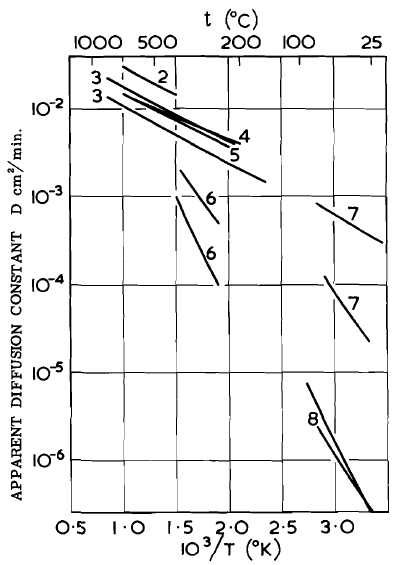
\includegraphics[width=\textwidth]{VAryingdiffuioncoeffinsteel.png}
        \caption{Varying order of diffusion coefficient by Darken and Smith experiment\cite{McNabb1963}.}
        \label{fig:diffusion_coeff}
    \end{subfigure}
    
    \caption{Hydrogen diffusion characteristics, illustrating the energy landscape of trap sites alongside the temperature dependence of the apparent diffusion constant.}
    \label{fig:combined_figure}
\end{figure}

Thus, based on these observations, they came up with the concepts of defects being ``traps'' that are basically potential energy wells at an energy level lower than that in the lattice positions. Hydrogen movement gets slowed down as they enter and leave these potential energy wells/traps, thus explaining the anomalous behavior of hydrogen in metals.

While Darken and Smith provided the foundational physical concept of hydrogen trapping, their original analytical approach was static and steady-state, leading subsequent researchers (such as McNabb \& Foster in 1963~\cite{McNabb1963} and Oriani in 1970~\cite{Oriani1970}) to develop transient kinetic rate laws for lattice-trap hydrogen interchange

Based upon the observations made by Darken and Smith, McNabb and Foster~\cite{McNabb1963} came up with a physical model where hydrogen randomly hops through normal interstitial lattice sites (NILS) obeying Fick's first law, but is delayed by a uniformly distributed population of localized potential energy wells (traps) of finite capacity. To describe this kinetic exchange, they formulated the coupled non-linear PDE Lattice-Trap Mass Balance:
\begin{equation}
    \frac{\partial C}{\partial t} + N \frac{\partial n}{\partial t} = \nabla \cdot (D \nabla C)
\end{equation}
separating mobile lattice concentration ($C$) from trapped hydrogen ($N n$, where $N$ is trap density and $n$ is fractional trap occupancy). Kinetic Exchange Rate Law:
\begin{equation}
    \frac{\partial n}{\partial t} = k C (1 - n) - p n
\end{equation}
where $k$ is the capture rate coefficient (proportional to vacant traps $1-n$ and mobile hydrogen $C$) and $p$ is the release/detrapping rate coefficient. There was, however, a discrepancy in the unit regarding the capture rate coefficient which will be explained as we move further onto work done by others.

They employed non-dimensionalisation and were able to come up with analytical solutions for key limiting transport regimes:
\begin{itemize}
    \item High-Concentration Limit ($C_0 \gg N$): Traps saturate ($n \to 1$), rendering trapping negligible and recovering standard Fickian diffusion.
    \item Low-Concentration Limit ($C_0 \ll N$): Trapping kinetics linearize.
    \item Permanent Sink Limit ($p \to 0$): Traps act as irreversible sinks.
    \item Local Thermodynamic Equilibrium Limit: For large times ($\alpha \tau \gg 1$), the kinetic system collapses into a single parabolic diffusion PDE governed by an algebraic local trap--lattice equilibrium relationship ($w = \frac{\alpha u}{1 + \beta u}$)---laying the mathematical foundation later generalized by Oriani (1970)~\cite{Oriani1970}.
\end{itemize}

They also found thickness also has a crucial role. By deriving mathematical solutions across simple geometries (slabs, cylinders), McNabb and Foster successfully gave the first quantitative physical explanation for non-steady-state transient outgassing, concentration-dependent effective diffusivities, and time-dependent hydrogen retention in metals. But the problem with the model came with these coupled PDEs being highly nonlinear, thus analytical solutions were impossible for general boundary conditions.

To in a way bypass the computational cost of solving the McNabb--Foster PDE, Oriani~\cite{Oriani1970} introduced the local thermodynamic equilibrium hypothesis ($\mu_L = \mu_T$). The way in which they reached this was by assuming that local trapping (capture) and detrapping (release) was much faster than hydrogen moving across the specimen; as a result, mobile and lattice local hydrogen concentration was always in equilibrium with each other. This led to a huge mathematical simplification as instead of solving two coupled diffusion equations, he combined lattice diffusion and trap kinetics into a single diffusion equation governed by a concentration-dependent Effective Diffusivity ($D_{\text{eff}}$).

By treating this, he was able to gain insights like at low hydrogen concentrations traps grab most of the hydrogen, thus making hydrogen transport very slow ($D_{\text{eff}} \ll D_L$) where $D_{\text{eff}}$ is the effective diffusion coefficient. As hydrogen concentration increases and traps fill up and saturate, hydrogen moves faster and $D_{\text{eff}}$ approaches the normal lattice speed ($D_L$). He was also able to explain why hydrogen desorbs from steel much slower than it enters. Near the surface, traps hold on to hydrogen as lattice concentration drops, creating a diffusion bottleneck. The limitation of it being that the local equilibrium assumption works great for steady-state or slow room-temperature diffusion; however, it breaks down during rapid TDS heating where temperature rises faster than traps can re-equilibrate.

The detailed formulations of both McNabb and Foster and Oriani's models are explained in the further section as it is the core of our numerical simulation model.

\section{Analysis of TDS Spectra}
\label{sec:analysis_of_tds}

Kissinger (1957) originally derived a first-order rate equation for differential thermal analysis of chemical reactions. Choo and Lee (1982) transferred this concept to hydrogen TDS by treating hydrogen escape from microstructural traps as a first-order chemical detrapping reaction. In TDS, a hydrogen-charged sample is heated at a constant linear heating rate ($\phi = dT/dt$), and the resulting surface desorption flux ($J$) is recorded as a function of temperature ($T$). The fundamental governing equation is expressed as:
\begin{equation}
    \ln\left(\frac{\phi}{T_{\text{peak}}^2}\right) = -\frac{E_d}{R T_{\text{peak}}} + \text{constant}
\end{equation}
where $T_{\text{peak}}$ is the peak desorption temperature ($\text{K}$) and $E_d = E_L + E_b$ is the total activation energy required for detrapping ($\text{J/mol}$). By performing TDS tests across multiple heating rates ($\phi$), the slope of $\ln(\phi/T_{\text{peak}}^2)$ versus $1/T_{\text{peak}}$ yields the apparent detrapping energy $E_d$.

\begin{figure}[htbp]
    \centering
    \includegraphics[width=0.7\textwidth]{"exampleleeandlee.png"}
    \caption{Example of a Choo-Lee plot illustrating the linear relationship between $\ln(\phi/T_c^2)$ and $1/T_c$, from which the activation energy for desorption ($E_d$) can be determined from the slope ($-E_d/R$)\cite{Wei2012}.}
    \label{fig:choo_lee_plot}
\end{figure}

However, there were certain flaws due to the assumptions made using this Kissinger peak shift analysis. They assume that desorption is controlled strictly by detrapping kinetics, neglecting the physical time required for detrapped hydrogen to diffuse across the specimen bulk to the surface ($D_L \to \infty$), or in other words, they assume infinitely fast spatial diffusion. They also ignore the effect of specimen thickness as established by Turnbull~\cite{Turnbull1997}, Legrand~\cite{Legrand2015}, and Drexler~\cite{Drexler2019}. The time taken for lattice diffusion $\tau_d \approx L^2 / (16 D_L)$ introduces a delay compared to infinitely fast diffusion. If the specimen thickness is greater than $L > 0.5\text{ mm}$, this spatial lag shifts $T_{\text{peak}}$ to higher temperatures independently of trap strength; consequently, most of the literature showed Kissinger analysis severely underestimating the true binding energy by 20\% to 50\%. The method is also unable to resolve overlapping peaks in the TDS curve, and it doesn't give any information regarding the trap site densities ($N_T$).

Turnbull (1997)~\cite{Turnbull1997} addressed these problems by using a continuum transport framework where he developed an extended 1D nonlinear transient continuum model coupling Fickian lattice diffusion with McNabb--Foster kinetic trapping and detrapping across one or more independent trap populations. He used implicit FDM as the numerical method to solve this coupled problem using an iterative TDMA solver over the 1D domain. The initial concentration of hydrogen was ($C_0$) across the specimen. He split the domain into 2 due to symmetry and enforced $\partial C/\partial x = 0$ at $x=0$, and an ideal zero-concentration vacuum condition ($C=0$) at the desorbing exit surface. By solving this coupled equation, he was able to find out that specimen thickness ($L$) severely shifts the peak desorption temperature. 

\begin{figure}[htbp]
    \centering
    % First subfigure
    \begin{subfigure}[b]{0.48\textwidth}
        \centering
        \includegraphics[width=\textwidth]{"tdsturnbull1.png"}
        \caption{Thermal desorption spectra for AISI 4340 with a single type of trap of binding energy $-48\text{ kJ mol}^{-1}$\cite{Turnbull1997}.}
        \label{fig:tds_single_trap}
    \end{subfigure}
    \hfill
    % Second subfigure
    \begin{subfigure}[b]{0.48\textwidth}
        \centering
        \includegraphics[width=\textwidth]{"tdsturnbull2.png"}
        \caption{Thermal desorption spectrum for two types of binding energies $-48$ and $-68\text{ kJ mol}^{-1}$ (equivalent site density)\cite{Turnbull1997}.}
        \label{fig:tds_two_traps}
    \end{subfigure}
    
    \caption{Simulated TDS taken from \cite{Turnbull1997}.}
    \label{fig:turnbull_tds}
\end{figure}

In thicker specimens, detrapped hydrogen takes longer to diffuse to the surface, thus delaying hydrogen release and shifting the peak temperature independent of the trap strength. He also found out that the height of the activation energy needed to enter a trap was shown to have only a slight effect on the TDS spectrum compared to binding energy and trap site density.

There was a dimensional inconsistency in McNabb and Foster's original formulation; the solvent interstitial lattice site density ($N_L$) was implicitly merged into the capture rate parameter $k$. This created a dimensional discrepancy where capture rate $k$ carried units of $\text{m}^3 \cdot \text{mol}^{-1} \cdot \text{s}^{-1}$, whereas release rate $p$ had units of $\text{s}^{-1}$. Krom and Bakker~\cite{Krom2000} pointed out that from a dimensional viewpoint, having different units for trapping and detrapping was mathematically inconsistent. His work also explained about the uncertainty of Oriani's local thermodynamic equilibrium hypotheses during mechanical deformation---whether we could assume if local equilibrium was maintained or whether full kinetic rate equations were required. His work showed that indeed for standard tensile testing with strain rates ($\dot{\epsilon}_p \approx 10^{-4}\text{ to } 1\text{ s}^{-1}$), the rate of hydrogen transfer into newly generated dislocation traps easily keeps pace with plastic strain rate, thus the local equilibrium assumption can be held valid. The work also showed how we could couple plastic strain-dependent dislocation trap density with continuum mass transport models. The governing equations for this are also given in the next section.

\begin{figure}[htbp]
    \centering
    \includegraphics[width=0.7\textwidth]{"kromimage"}
    \caption{Plot showing the ratio of trapped hydrogen concentration to equilibrium concentration ($C_T/C_{T,eq}$) as a function of plastic strain ($\varepsilon_p$), with trap density ($N_T$) depending on the strain. Parameters used: $\Delta E_T = -60\text{ kJ/mol}$, $C_{\text{tot}} = 3 \times 10^{21}\text{ m}^{-3}$, $N_L = 5.1 \times 10^{29}\text{ m}^{-3}$, $T = 293\text{ K}$, $E_D = 6.9\text{ kJ/mol}$, and $v = 1 \times 10^{13}\text{ s}^{-1}$ \cite{Krom2000}.}
    \label{fig:krom_strain}
\end{figure}

It is now known that sample thickness affects the amount of hydrogen desorption from the sample, but the critical sample thickness beyond which classical Kissinger analysis and peak deconvolution fail and underestimate trap binding energy remained unquantified. Also, another problem with the TDS technique was that it only measures the total surface desorption flux ($\Delta C$). Without numerical modeling, it was impossible to directly verify whether Gaussian curve fitting accurately quantifies the true ratio of mobile lattice hydrogen ($\langle C_L \rangle$) to trapped hydrogen ($\langle C_T \rangle$). Legrand et al.~\cite{Legrand2015} implemented a 1D transient finite element method (FEM) transport model in COMSOL Multiphysics to study the effect across various sample thicknesses ($d$): $0.1\text{ mm}$ to $10\text{ mm}$, heating ramp rates ($\phi$): $1\text{ K/min}$ to $1000\text{ K/min}$, and untrapping frequencies ($\nu_T$): $0.1\text{ GHz}$ to $10\text{ THz}$ for martensitic steel. They compared the true computed evolution rates of lattice ($\Delta C_L$) and trapped ($\Delta C_T$) hydrogen against values extracted via standard Gaussian and Asymmetric Double Sigmoidal curve deconvolutions. By doing this, they were able to identify that below a specimen thickness of 4 mm, Kissinger plots accurately extract the true physical trap binding energy; beyond this critical value, spatial diffusion creates a transport lag and thus the Kissinger method leads to underestimation of binding energy with the underestimation being up to 50 percent.

He also emphasized that standard Gaussian deconvolution severely miscalculated the trapped to lattice concentration ratio, leading to overestimation or underestimation depending on the heating rate. Another crucial finding was related to the jump frequency associated with trapping ($\nu_L$) and detrapping ($\nu_T$): there was a necessity to keep $\nu_T < \nu_L$ so as to maintain the correct physical sequence where shallowly trapped hydrogen desorbs prior to deeply trapped hydrogen.

The effect of this trapping and detrapping jump frequency was further studied by Cheng et al. (2018)~\cite{Cheng2018}, where he studied under what physical boundaries (jump rate pre-factors $p_0, k_0$, trap binding energy $E_b$, specimen thickness $L$, and matrix diffusivity $D_L$) it was required to guarantee local equilibrium during transient transport. He found that for a 1 mm steel sample with $E_b = 27\text{ kJ/mol}$ and $m = 10^{-3}$, local thermodynamic equilibrium is achieved across the entire specimen when $p_0 \ge 5.0 \times 10^5\text{ s}^{-1}$. At this threshold, simulated McNabb--Foster curves become invariant and overlap perfectly with Oriani equilibrium. For stronger traps ($E_b = 42.14\text{ kJ/mol}$), a higher frequency threshold of $p_0 \ge 2.2 \times 10^8\text{ s}^{-1}$ is required, whereas for deep traps in his case $E_b \ge 67\text{ kJ/mol}$ (at room temperature), it requires $p_0 \ge 1.0 \times 10^{13}\text{ s}^{-1}$. Since $10^{13}\text{ s}^{-1}$ equals the maximum physical attempt (Debye) frequency $\nu$, traps cannot equilibrate with lattice hydrogen at room temperature, effectively making them trapped there.

\begin{figure}[htbp]
    \centering
    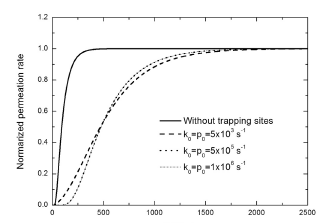
\includegraphics[width=0.75\textwidth]{lit_cheng_permeation_p0.png}
    \caption{Normalized permeation rate against time, simulated with the McNabb--Foster model for different values of the jump-frequency pre-factors $k_0 = p_0$, and compared with the curve without trapping sites. The curves for $k_0 = p_0 = 5\times10^{5}~\mathrm{s^{-1}}$ and $1\times10^{6}~\mathrm{s^{-1}}$ lie on top of each other, which shows that local equilibrium between lattice and trapped hydrogen has been reached. The curve for $k_0 = p_0 = 5\times10^{3}~\mathrm{s^{-1}}$ does not overlap with them, so local equilibrium is not reached for this value. ~\cite{Cheng2018}}.
    \label{fig:cheng_p0}
\end{figure}

Drexler~\cite{Drexler2019} modeled hydrogen transport across a 1 mm thick disc specimen using a multi-trap continuum framework; he assessed local thermodynamic equilibrium between lattice sites and $n_t$ independent trap populations. He implemented it in the commercial finite element code 3DS ABAQUS using custom user element subroutines (UEL) and standard 1D heat/mass transfer elements (DC1D2). He then coupled ABAQUS with a Python optimization pipeline using scipy.optimize (Scipy.Optimize.Leastsq / Nelder--Mead algorithm). Drexler et al.~\cite{Drexler2019} calibrated and validated their framework on three Fe-C-Ti model alloys containing 0.1, 0.2, and 0.3 wt\% C with stoichiometric Ti additions. His study was on how heat treatment changes the microstructure of an Fe-C-Ti alloy and how it changes the trap environment. His first quenched alloy produced a martensitic structure with lath boundaries that acted as weak traps; then he tempered the material at $600^\circ\text{C}$ for 1 hour, which causes fine TiC precipitates to form. This introduces new interfaces and carbon vacancies. He was able to observe 5 different types of traps ranging from 15 kJ/mol to 110 kJ/mol, which he then compared with literature first-principle calculations and characterized. He also was able to see the 5th trap disappearing at prolonged 2 hours of tempering, which he attributed to carbon vacancies disappearing due to diffusion of carbon atoms. Thus, he was able to effectively quantify several trap features by numerically modeling the TDS spectrum.

One of the important factors that comes into the picture while numerical modeling is boundary conditions. The widely employed boundary condition was the Dirichlet boundary condition. Traditional crack tip hydrogen models such as Sofronis and McMeeking (1989) rely on prescribing a fixed, constant lattice hydrogen concentration ($C_L = C_0$) at the crack faces. This assumes instantaneous infinite-rate electrochemical surface reactions and ignores the real adsorption-absorption kinetics operating at the metal-electrolyte interface. Also, the fixed boundary conditions are independent of stress, failing to capture how elevated crack tip hydrostatic stress enhances chemical potential and draws higher surface fluxes into the fracture zone. They also said that if we assume Conventional Plasticity ($J_2$ Flow Theory) near the crack tip, it cannot account for the huge strain gradients, and since geometrically necessary dislocations (GNDs) are directly proportional to these large strain gradients, this means more traps for hydrogen. These GNDs also elevate hydrostatic stress beyond classical limits, which strongly affects the hydrogen accumulation. Mart\'{\i}nez-Pa\~{n}eda et al.~\cite{MartinezPaneda2020} implemented a fully coupled, multi-physics finite element framework in 2D plane strain (built in ABAQUS via custom subroutines). The model solved the mechanical equilibrium equation, transient McNabb--Foster mass transport, and trapping kinetic PDEs concurrently, taking displacements ($u, v$), lattice hydrogen concentration ($C_L$), and trap occupancy ($\theta_r$) as nodal degrees of freedom. They replaced Dirichlet constant concentration schemes with Neumann generalized absorption flux boundary conditions:
\begin{equation}
    J_{\text{in}} = k_{\text{abs}} N_s \theta_{\text{ad}} - k_{\text{des}} C_s (1 - \theta_{\text{ad}})
\end{equation}
where $N_s$ is absorption site density, $C_s$ is subsurface concentration, and surface coverage $\theta_{\text{ad}}$ is calculated dynamically by balancing the Hydrogen Evolution Reaction (HER) kinetics (Volmer--Heyrovsky--Tafel steps):
\begin{multline}
    k_{r,\text{chem}} \theta_{\text{ad}}^2 + \left( k_{\text{abs}} \exp\left[ \frac{V_H \sigma_h}{RT} \right] + k_{\text{des}} C + k_c + k_{r,\text{elec}} \right) \theta_{\text{ad}} \\
    - k_{\text{des}} C - k_c = 0
\end{multline}
This formulation explicitly couples subsurface hydrogen entry flux ($J_{\text{in}}$) with applied overpotential ($\eta$), charging current ($k_c$), recombination rates ($k_{r,\text{chem}}, k_{r,\text{elec}}$), and local hydrostatic stress ($\sigma_h$).

E. Garc\'{\i}a-Mac\'{\i}as, Z. D. Harris, and E. Mart\'{\i}nez-Pa\~{n}eda (2024) came up with an open-sourced GUI-based platform in MATLAB designed for simulating virtual TDS tests and analyzing experimental spectra. The model gave the option to choose both Oriani's model and the McNabb--Foster model. The McNabb--Foster model is capable of solving lattice concentration and 6 independent trap concentrations using a 1D finite difference method coupled with MATLAB's ode15s solver: a variable-order solver based on numerical differentiation formulas optimized for stiff problems. Oriani's local equilibrium was solved using MATLAB's pdepe solver (based on the method of lines). To extract trapping parameters from experimental curves, they embedded an inverse fitting tool based on Particle Swarm Optimization (PSO). The objective function minimizes the Root Mean Squared Error (RMSE) between experimental flux/desorption rates and numerical predictions:
\begin{equation}
    \text{RMSE} = \sqrt{\frac{1}{N} \sum_{i=1}^{N} \left( \Delta C_{\text{exp}}(T_i) - \Delta C_{\text{sim}}(T_i, \boldsymbol{\theta}) \right)^2}
\end{equation}
where the optimization vector $\boldsymbol{\theta} = [\Delta H^{(1)}, N_T^{(1)}, \dots, \Delta H^{(n_t)}, N_T^{(n_t)}]$ searches across global search bounds (e.g., $-150 \le \Delta H \le -15 \text{ kJ/mol}$). They observed that for jumping frequency $\nu \ge 10^8\text{ Hz}$, trapping kinetics become faster than spatial diffusion, causing McNabb--Foster curves to perfectly overlap with Oriani's thermodynamic equilibrium. He also highlighted the importance of rest time, that is the time taken to take the sample from the charging apparatus to the testing apparatus, which he also incorporated in his model. His parametric sensitivity analysis revealed that predicted TDS spectra were highly insensitive to initial concentration but highly dependent on rest time.

The problem with conventional inverse TDS optimization algorithms such as Particle Swarm Optimization (PSO) or Nelder--Mead methods was the requirement of knowing the exact number of trap types ($n_t$) a priori; if it is misidentified, the optimization algorithm can yield unsatisfactory or unphysical parameter fits even if it converges. Also, we had to give initial parameter guesses ($E_b, N_T$) being close to true values; otherwise, they frequently converge to unphysical local minima. Furthermore, iterative optimization requires running dozens to hundreds of forward finite element (FEM) simulations from scratch for every new experiment, without the ability to reuse past simulation data. These issues were identified by Marrani et al.~\cite{Marrani2025}; they developed a two-stage deep learning framework implemented in Keras/TensorFlow comprising two multi-layer fully connected feed-forward Artificial Neural Networks trained with backpropagation. The first classification network predicts the discrete number of active trap types, whereas the second regression network, trained specifically for $n_t$, computes absolute binding energies ($\vert{}\Delta H^{(i)}\vert{}$) and trap site densities ($N_T^{(i)}$). The approach they used to train the model was synthetically generated training data; they developed a 1D transient finite element transport solver in Python capable of solving both McNabb--Foster trapping kinetics and Oriani local equilibrium. The method they employed was capable of extracting binding energy and trap density for AISI 4340 Steel (Novak et al.~\cite{Novak2010}) and Fe--C--Ti \& Fe--C--Ti--Ni Model Alloys. The model, however, struggled to identify traps if the trap density spanned more than 2 orders of magnitude. Also, the major issue of this ML model was that if we change any specific parameter like specimen thickness ($L$), heating rate ($\phi$), and lattice diffusivity ($D_L$) used during training data generation, we had to train a new model with modified parameters from scratch.

Another ML technique was used by Yang et al. (2025)~\cite{Yang2025}; they implemented an extended dimensionless Oriani local equilibrium transport solver in MATLAB using the pdepe solver to rapidly generate synthetic TDS desorption spectra across wide ranges of normalized trap densities ($\bar{N} \in [10^{-6}, 10^{-2}]$) and binding energies ($\Delta \bar{H} \in [-28, -13.5]$). They converted the continuous TDS curves into a compact input representation without losing shape details; they parameterized the desorption peaks using a 5-parameter Asymmetric Double Sigmoid Function (ADSF). They fitted the original TDS curve to find the values of these parameters. They compared 7 optimization algorithms (PSO, WOA, GWO, GA, SSA, DBO, SCA) to fit the ADSF and found out that Grey Wolf Optimization (GWO) achieved the highest rank in accuracy and convergence speed. Using the 5 ADSF parameters ($P_1 \dots P_5$) as input features and normalized trap density ($\bar{N}$) \& binding energy ($\Delta \bar{H}$) as target outputs, they constructed and evaluated 4 machine learning algorithms: Multi-Layer Perceptron (MLP-BP), Random Forest (RF), Light Gradient Boosting (LGBM), and Support Vector Regression (SVR), with Bayesian optimization used for hyperparameter tuning. Among the evaluated machine learning algorithms, Support Vector Regression (SVR) demonstrated superior predictive performance.

\section{Hydrogen Trapping in X65 Steel}
\label{sec:hydrogen_trapping_x65}

Understanding how hydrogen enters X65 steel and subsequently interacts with the lattice and defects present within the material is crucial. Cheng (2007) studied commercial API 5L X65 linepipe steel with a ferritic-pearlitic matrix microstructure. He used a standard Devanathan--Stachurski double electrochemical cell operated at ambient room temperature for his permeation experiments. He calculated that the effective diffusivity varied in the range of $1.5 \times 10^{-7}\text{ cm}^2/\text{s}$ to $2.0 \times 10^{-5}\text{ cm}^2/\text{s}$ depending on subsurface charging current density and surface passivation state. This was significantly lower than the intrinsic lattice diffusivity of pure iron ($D_L \approx 7 \times 10^{-5}\text{ cm}^2/\text{s}$), thus confirming that microstructural traps do slow down the movement of hydrogen through the sample.

The variation in the effective diffusivity was addressed by Fallahmohammadi, Bolzoni, and Lazzari (2013)~\cite{Fallahmohammadi2013}, where they tried to resolve the discrepancy between the true lattice diffusivity and the apparent or effective diffusivity. They tested API 5L X65 steel and compared it against low-alloy ASTM A182 F22 steel. The composition of the X65 steel was $0.11\text{ wt\% C}$, $0.28\text{ wt\% Si}$, $1.18\text{ wt\% Mn}$, $0.007\text{ wt\% S}$, $0.017\text{ wt\% P}$, and $0.17\text{ wt\% Cr}$, with a ferritic-pearlitic matrix.

To measure the true lattice diffusivity without trap-filling interference, they first saturated the sample with an initial steady-state permeation current density. Then, the cathodic current was increased in steps. By doing so, since the traps were already saturated during the initial steady state, they were able to isolate mobile lattice migration. They observed that the true lattice diffusivity obtained was $D_L \approx 2.3 \times 10^{-10} \text{ m}^2/\text{s}$. Another observation they made was that at room temperature, irreversible traps did not play a significant effect in slowing the diffusion time.

\begin{table}[htbp]
\centering
\tablestyle
\caption{Common hydrogen traps their trapping energies (in $E_b$) in BCC steels~\cite{Li2022}.}
\label{tab:traps}
\fitwidth{
\begin{tabular}{@{}lL{2cm}L{3cm}L{6.5cm}@{}}
\toprule
Trap type & Binding energy ($-E_b$, kJ/mol) & Characterization technique & Reference \\
\midrule
\multicolumn{4}{@{}l}{\textbf{Solute elements}} \\
Si, Cr, Mn, Co and Mo & $\sim$0 & First Principle & Counts et al. (2010) \\
C (interstitial) & 9 & First Principle & Counts et al. (2010) \\
N (interstitial) & 13 & Magnetic Relaxation & Au \& Birnbaum (1978) \\
Nb & $-7$ (repulsive) & First Principle & Counts et al. (2010) \\
Ti & $-8$ & First Principle & Counts et al. (2010) \\
Mg & $-15$ & First Principle & Counts et al. (2010) \\
Sc & $-20$ & First Principle & Counts et al. (2010) \\
Y & $-25$ & First Principle & Counts et al. (2010) \\
\addlinespace
\multicolumn{4}{@{}l}{\textbf{Crystal defects}} \\
Single vacancy & 24--78 & First Principle, Permeation & Counts et al. (2010); Kim et al. (1985); Kim and Pyun (1982); Myers et al. (1979); Paxton (2014) \\
Micro-voids & 40 & TDA & Lee \& Lee (1983) \\
Dislocations (bulk) & 60 & Permeation & Kumnick \& Johnson (1980) \\
Screw dislocations & 26 & First Principle & Paxton \& Katzarov (2016) \\
Dislocation strain field & 12--27 & Permeation, TDA & Choo and Lee (1982); Hagi and Hayashi (1987); Takai et al. (1996) \\
GB & 9--49 & Mechanical Analysis, TDA & Bernstein (1974); Choo and Lee (1982); Lin et al. (2019); Ono and Meshii (1992) \\
Prior austenite GB & 47 & Permeation & Parvathavarthini et al. (2001) \\
\addlinespace
\multicolumn{4}{@{}l}{\textbf{Second phases}} \\
Incoherent TiC & 60--129 & Permeation, TDA & Asaoka et al. (1978); Lee and Lee (1984); P\'{e}rez Escobar et al. (2013); Pressouyre and Bernstein (1978); Wei and Tsuzaki (2006) \\
Semi-coherent TiC & 48 & TDA & Wei \& Tsuzaki (2006) \\
Incoherent V$_4$C$_3$ & 40 & TDA & Lin et al. (2021) \\
Semi-coherent V$_4$C$_3$ & 25--28 & TDA & Asahi et al. (2003); Yamasaki and Takahashi (1997) \\
Incoherent NbC & 55--60 & TDA & Wallaert et al. (2014) \\
Semi-coherent NbC & 28--56 & TDA & Wallaert et al. (2014); Wei and Tsuzaki (2009) \\
Coherent Mo$_2$C & 11--34 & TDA & Depover and Verbeken (2016); Hinotani et al. (1985); Thomas et al. (2002) \\
Cementite/$\alpha$ interface & 11--18 & Permeation, TDA & Choo and Lee (1982); Hong and Lee (1983); Wei and Tsuzaki (2005) \\
$\epsilon$ carbide & 12--65 & Permeation, TDA & Hsu et al. (2020); Serra et al. (1997) \\
$\epsilon$ copper & 27 & TDA & Lin et al. (2019) \\
Dispersed oxide & 45 & Permeation, First Principle & Esteban et al. (2007); Huang et al. (2020) \\
MnS interface & 64 & TDA & Lee and Lee (1983); Takai et al. (1996) \\
Austenite/Ferrite interface & 44 & Permeation & Turnbull \& Hutchings (1994) \\
Iron oxide interface & 43--62 & TDA & Lee et al. (1984) \\
Al$_2$O$_3$ interface & 71 & TDA & Lee \& Lee (1986) \\
\bottomrule
\end{tabular}
}
\end{table}

%================================================
% CHAPTER 3
%================================================
\chapter{Mathematical Formulation and Numerical Implementation}
\label{ch:formulation}

\section{Hydrogen Species and Concentration Variables}

Hydrogen within the ferritic steel matrix is separated into mobile lattice hydrogen and hydrogen trapped at microstructural defects.

\textbf{Interstitial lattice hydrogen}: These are the hydrogen atoms occupying the normal interstitial lattice sites of the body-centered cubic (BCC) $\alpha$-iron lattice. Here we assume it to be the tetrahedral voids~\cite{KIUCHI1983961}. This population is considered mobile and is responsible for the spatial diffusion through the steel matrix.

The lattice hydrogen concentration is denoted by
\begin{equation}
C_L = C_L(x, t),
\label{eq:ch3_CL}
\end{equation}
where $C_L$ represents the molar concentration of mobile lattice hydrogen, with units of $[C_L] = \mathrm{mol~m^{-3}}$. The corresponding density of normal interstitial lattice sites is denoted by $N_L$, also expressed on a molar-volume basis in the present formulation, with $[N_L] = \mathrm{mol~m^{-3}}$.

\textbf{Trapped hydrogen}: Hydrogen may also be captured by microstructural defects that act as energetically favourable trapping sites, for example dislocations, vacancies, grain boundaries, interfaces and other microstructural features capable of forming local potential energy wells.

Each trap population is associated with its own site density $N_T^{(i)}$, and $n_t$ is the number of trap populations. The concentration of hydrogen associated with the $i$-th trap population is written as
\begin{equation}
C^{(i)}_T = C^{(i)}_T(x, t), \quad i = 1, 2, \dots , n_t,
\label{eq:ch3_CT}
\end{equation}
with $[C^{(i)}_T] = \mathrm{mol~m^{-3}}$.

The total hydrogen concentration at a given location is consequently
\begin{equation}
C_H(x, t) = C_L(x, t) + \sum_{i=1}^{n_t} C^{(i)}_T(x, t).
\label{eq:ch3_CH}
\end{equation}

The distinction between lattice and trapped populations is important because the traps exchange hydrogen only with the lattice population, and the hydrogen distributes itself among the different traps according to their binding energies.

\textbf{Lattice occupancy}: The fractional occupancy of normal interstitial lattice sites is defined as
\begin{equation}
\theta_L(x, t) = \frac{C_L(x, t)}{N_L}.
\label{eq:ch3_thetaL}
\end{equation}

Similarly, the fractional occupancy of the $i$-th trap population is
\begin{equation}
\theta^{(i)}_T(x, t) = \frac{C^{(i)}_T(x, t)}{N^{(i)}_T}, \quad i = 1, 2, \dots , n_t,
\label{eq:ch3_thetaT}
\end{equation}
where $N^{(i)}_T$ is the total density of available sites belonging to the $i$-th trap population.

\section{Fundamental Physical Assumptions}

The following assumptions are made in modelling this physical system:

\begin{enumerate}
    \item \textbf{One-dimensional transport}: hydrogen transport occurs only along the specimen thickness coordinate $x$.
    \item \textbf{Isotropic and homogeneous matrix}: the material properties are assumed to be independent of spatial coordinate.
    \item \textbf{Fixed trap population}: the number density of trap sites $N^{(i)}_T$ remains constant throughout the simulation,
    \begin{equation}
    \frac{\partial N^{(i)}_T}{\partial t} = 0.
    \label{eq:ch3_NT_const}
    \end{equation}
    Trap generation, annihilation, and microstructural phase transformations are therefore not considered.
    \item \textbf{Non-interacting trap populations}: we assume that hydrogen in two traps do not interact directly; they exchange hydrogen only via the diffusing hydrogen.
    \item \textbf{Fickian lattice diffusion}: only the mobile lattice population contributes directly to the spatial diffusion flux.
    \item \textbf{Stress-free desorption formulation}: hydrogen movement due to hydrostatic stress gradients is neglected.
    \item \textbf{Uniform instantaneous temperature}: the specimen is assumed to have a spatially uniform temperature $T(t)$ at each instant, and no heat transfer calculation is carried out to obtain it.
\end{enumerate}

\section{Modelling Framework}

The present formulation is a one-dimensional, multi-trap, non-isothermal transient hydrogen transport model based on McNabb--Foster kinetic trapping and detrapping, with an Oriani local-equilibrium condition used to establish the initial hydrogen distribution, i.e.\ Oriani local equilibrium gives how the total concentration is split between the traps and lattice if we assume that the sample is held for enough time so that the lattice and traps have enough time to equilibrate and settle down.

McNabb--Foster kinetics tells us how the time-dependent concentration variation occurs in the lattice and traps based on trapping, detrapping and diffusion processes.

One thing to be noted is that in the following sections, notations and parameters are taken as they are from the source literature along with their corresponding definitions.

\section{Hydrogen Diffusion}

\subsection{Fickian Lattice Flux}

The spatial transport of mobile interstitial hydrogen through the normal lattice sites is described by Fick's first law~\cite{Fallahmohammadi2013,Legrand2015,MartinezPaneda2020}:
\begin{equation}
J_L(x, t) = -D_L(T) \frac{\partial C_L(x, t)}{\partial x},
\label{eq:ch3_JL}
\end{equation}
where $J_L$ is the lattice hydrogen flux and $D_L(T)$ is the temperature-dependent lattice diffusion coefficient.
The units are
\begin{equation}
[J_L] = \mathrm{mol~m^{-2}~s^{-1}},
\label{eq:ch3_JL_units}
\end{equation}
and
\begin{equation}
[D_L] = \mathrm{m^2~s^{-1}}.
\label{eq:ch3_DL_units}
\end{equation}
The negative sign indicates that hydrogen diffuses from regions of higher lattice concentration toward regions of lower lattice concentration.

\subsection{Temperature-Dependent Lattice Diffusivity}

The lattice diffusion coefficient is described by an Arrhenius temperature dependence:
\begin{equation}
D_L(T) = D_0 \exp\left( -\frac{E_L}{RT(t)} \right),
\label{eq:ch3_DL}
\end{equation}
where $D_0$ is the pre-exponential diffusion coefficient and $E_L$ is the activation energy for lattice diffusion. Their units are
\begin{equation}
[D_0] = \mathrm{m^2~s^{-1}}, \quad [E_L] = \mathrm{J~mol^{-1}}.
\label{eq:ch3_D0_units}
\end{equation}
The universal gas constant is
\begin{equation}
R = 8.31446 \mathrm{~J~mol^{-1}~K^{-1}},
\label{eq:ch3_R}
\end{equation}
and $T(t)$ is the absolute temperature in kelvin.

The temperature dependence of $D_L$ provides the coupling between the thermal history and the rate of lattice hydrogen transport.

\section{McNabb and Foster Trapping Kinetics}

To replace classical diffusion theory, McNabb and Foster~\cite{McNabb1963} introduced a physical state description characterized by four core parameters ($D$, $N$, $k$, and $p$).

The four core physical parameters are

\textbf{True Lattice Diffusion Constant ($D$)}: The classical Fickian diffusion constant. $D$ is constant at a given temperature and independent of concentration, trap occupancy, or position.

\textbf{Active Trap Density ($N$)}: The uniform concentration of active traps (number of traps per unit volume).

\textbf{Capture Parameter ($k$)}: It is a rate constant governing how the diffusing hydrogen atoms are captured by vacant traps.
It is postulated that the number of atoms captured per second in a volume element $\delta V$ is proportional to the diffusing concentration ($C$) and the concentration of vacant traps ($N(1 - n)$): $kCN(1 - n)\delta V$.

\textbf{Release Probability ($p$)}: The mean probability that an occupied trap will release its hydrogen atom in any given second. It is dependent on the temperature of the specimen and the activation energy, but is independent of the local concentration of trapped or diffusing hydrogen.
The number of atoms released per second in a small volume element $\delta V$ is proportional to the occupied traps: $pnN\delta V$.

\subsection{Derivation of McNabb--Foster Trapping Kinetics}

Consider the flux of hydrogen atoms through the bounding surface $S$ of an arbitrary volume $V$ of an isotropic homogeneous medium containing $N$ traps per unit volume.

\noindent $C(x, t)$: Concentration of diffusing atoms.\\
\noindent $n(x, t)$: Fraction of active traps containing hydrogen atoms.

The effective number of hydrogen atoms $Q(t)$ in $V$ at time $t$ is:
\begin{equation*}
\iiint_V (C + nN) \, dV
\end{equation*}
The rate of increase $dQ/dt$ is equal to the flux of atoms through $S$ per second, that is:
\begin{equation*}
\frac{dQ}{dt} = \iint_S D(\text{grad } C) \cdot \mathbf{n} \, dS
\end{equation*}
where $\mathbf{n}$ is the outward unit normal to $S$. Applying the Divergence Theorem, we obtain:
\begin{equation*}
\iiint_V \left( \frac{\partial C}{\partial t} + N \frac{\partial n}{\partial t} \right) dV = \iiint_V \text{div}(D \text{ grad } C) \, dV
\end{equation*}
Since this equation is valid for any control volume $V$, the integrands can be equated to give the partial differential equation:
\begin{equation}
\frac{\partial C}{\partial t} + N \frac{\partial n}{\partial t} = \text{div}(D \text{ grad } C)
\label{eq:ch3_mf_pde}
\end{equation}
The second equation considers the rate of interchange of hydrogen atoms between the trapped and diffusing populations:
\begin{equation*}
N \frac{\partial n}{\partial t} = kCN(1 - n) - pnN
\end{equation*}
Simplifying yields the second coupled equation:
\begin{equation}
\frac{\partial n}{\partial t} = kC(1 - n) - pn
\label{eq:ch3_mf_trap}
\end{equation}

By non-dimensionalising these equations, McNabb and Foster also presented analytical solutions for different regimes.

\section{Krom and Bakker Model}

Krom and Bakker~\cite{Krom2000} developed a hydrogen diffusion and trapping formulation based on the same physical principle as McNabb and Foster, and they expressed the trapping kinetics in terms of the fractional occupancy of lattice and trap sites. By doing so they were able to get a dimensionally consistent form of the trapping and detrapping processes.

\subsection{Dimensional Consistency of the McNabb--Foster Formulation}

In the McNabb--Foster model, the rate of change of trap occupancy is given by Equation~\eqref{eq:ch3_mf_trap}, where $n$ is the fraction of occupied traps, $C$ is the concentration of diffusing hydrogen, $k$ is the capture rate coefficient and $p$ is the release rate constant.

Since $n$ is dimensionless, the units of the left-hand side are
\begin{equation}
\left[\frac{\partial n}{\partial t}\right] = \mathrm{s}^{-1}.
\label{eq:ch3_n_units}
\end{equation}
The release term must have the same units. Since $n$ is dimensionless, the units of $p$ are
\begin{equation}
[p] = \mathrm{s}^{-1}.
\label{eq:ch3_p_units}
\end{equation}
The trapping term must also have units of inverse time. Therefore,
\begin{equation}
[kC] = \mathrm{s}^{-1}.
\label{eq:ch3_kC_units}
\end{equation}
If hydrogen concentration is expressed in $\mathrm{mol~m^{-3}}$, the capture coefficient must have units
\begin{equation}
[k] = \mathrm{m^3~mol^{-1}~s^{-1}}.
\label{eq:ch3_k_units}
\end{equation}
Similarly, if concentration is expressed in atoms per cubic metre, the units become $\mathrm{m^3~atom^{-1}~s^{-1}}$.

Thus, the capture coefficient and release rate constant have different units in the original McNabb--Foster kinetic equation.

\subsection{Dimensionally Consistent Kinetic Formulation}

The fractional occupancies of the normal interstitial lattice sites and of the trap sites, $\theta_L$ and $\theta_T$, are defined in Equations~\eqref{eq:ch3_thetaL} and~\eqref{eq:ch3_thetaT} (the index $i$ is dropped here, since a single trap population is considered). Both are dimensionless quantities. The concentration of vacant trap sites is $N_T(1-\theta_T)$. The trapping rate can therefore be expressed in terms of the lattice occupancy and the fraction of vacant traps.

The resulting kinetic equation is
\begin{equation}
\frac{\partial C_T}{\partial t} = N_T k\theta_L(1-\theta_T)-lC_T,
\label{eq:ch3_kb_trap}
\end{equation}
where $k$ and $l$ are the trapping and detrapping frequency coefficients, respectively, with units of $\mathrm{s}^{-1}$.

Substituting $C_T=N_T\theta_T$ into Equation~\eqref{eq:ch3_kb_trap} gives
\begin{equation}
N_T\frac{\partial\theta_T}{\partial t} = N_Tk\theta_L(1-\theta_T)-lN_T\theta_T.
\label{eq:ch3_kb_sub}
\end{equation}
Assuming a constant trap density and dividing by $N_T$, the kinetic equation becomes
\begin{equation}
\frac{\partial\theta_T}{\partial t} = k\theta_L(1-\theta_T)-l\theta_T.
\label{eq:ch3_kb_theta}
\end{equation}
In this formulation, the trapping and detrapping terms both have units of inverse time. The trapping term depends on the fraction of hydrogen occupying lattice sites and the fraction of vacant traps, whereas the detrapping term depends on the fraction of occupied traps.

\section{Oriani Local Equilibrium Model}

For a system in local thermodynamic equilibrium~\cite{Oriani1970}, the activities of hydrogen in the lattice and trap populations are related through an equilibrium constant $K_T$.
\begin{equation}
K_T = \frac{\theta_T/(1-\theta_T)}{\theta_L/(1-\theta_L)}.
\label{eq:ch3_K_def}
\end{equation}
For hydrogen in steel, the fractional occupancy of normal lattice sites is usually very small, such that $\theta_L\ll1$. Therefore, $1-\theta_L\approx1$, and Equation~\eqref{eq:ch3_K_def} reduces to
\begin{equation}
\frac{\theta_T}{1-\theta_T} = K_T\theta_L.
\label{eq:ch3_K_dilute}
\end{equation}
Rearranging gives
\begin{equation}
\theta_T = K_T\theta_L(1-\theta_T).
\label{eq:ch3_th_rearr}
\end{equation}
Collecting the terms containing $\theta_T$,
\begin{equation}
\theta_T(1+K_T\theta_L) = K_T\theta_L.
\label{eq:ch3_th_collect}
\end{equation}
Hence, the fractional occupancy of the trap sites is
\begin{equation}
\boxed{
\theta_T = \frac{K_T\theta_L}{1+K_T\theta_L}
}.
\label{eq:ch3_oriani}
\end{equation}
This equation shows the trap occupancy is given by the local lattice occupancy, the trap binding energy and the temperature using the equilibrium constant. As the lattice occupancy increases, the trap occupancy increases, approaching unity as the traps become saturated.

The equilibrium constant is related to the binding energy of a particular trap. If $\Delta H_i$ denotes the enthalpy change on trapping hydrogen at the $i$-th trap, the positive binding energy $E_b^{(i)}$ of that trap is defined as
\begin{equation}
E_b^{(i)}=-\Delta H_i,
\qquad
E_b^{(i)}>0
\quad\text{for an attractive trap},
\label{eq:ch3_binding_energy_convention}
\end{equation}
with $[E_b^{(i)}]=\mathrm{J~mol^{-1}}$. The equilibrium constant of the $i$-th trap is then
\begin{equation}
K_T^{(i)} = \exp\left(-\frac{\Delta H_i}{RT}\right) = \exp\left(\frac{E_b^{(i)}}{RT}\right),
\label{eq:ch3_K_energy}
\end{equation}
where $R$ is the universal gas constant and $T$ is the absolute temperature.

A larger binding energy corresponds to a larger equilibrium constant at a given temperature, thus hydrogen occupies that trap more. As temperature increases, it can be seen that the equilibrium preference for trapping decreases for a fixed binding energy.

\section{Application to the Present Model}

\subsection{Initial Trap Occupancy}

For multiple trap populations, the initial occupancy of trap population $i$ is obtained from the Oriani equilibrium relation, Equation~\eqref{eq:ch3_K_def}, without using the dilute approximation $1-\theta_L\approx1$,
\begin{equation}
\theta_{T,0}^{(i)} = \frac{K_T^{(i)}\theta_{L,0}}{1+\left(K_T^{(i)}-1\right)\theta_{L,0}},
\label{eq:ch3_theta_init}
\end{equation}
where $\theta_{L,0}=C_{L,0}/N_L$ is the initial lattice occupancy. For $\theta_{L,0}\ll1$ this reduces to Equation~\eqref{eq:ch3_oriani}. The initial lattice concentration $C_{L,0}$ is defined in Section~\ref{sec:ch3_bc}.

\subsection{Trapping Kinetics}

The exchange of hydrogen between the mobile lattice and each trap population during the thermal heating process is described using a similar formulation taken from~\cite{Marrani2025,MartinezPaneda2020}.

For the $i$-th trap population,
\begin{equation}
\frac{\partial C_T^{(i)}}{\partial t}
=
j_{\mathrm{trap}}^{(i)}
=
k_i(T)
\frac{N_T^{(i)}}{N_L}
C_L
\left(
1-\frac{C_T^{(i)}}{N_T^{(i)}}
\right)
-
p_i(T)
C_T^{(i)}
\left(
1-\frac{C_L}{N_L}
\right),
\label{eq:ch3_mcnabb_molar}
\end{equation}
where $k_i(T)$ is the trapping rate coefficient and $p_i(T)$ is the detrapping rate coefficient, both with units of $\mathrm{s^{-1}}$.

The first term represents hydrogen transfer from the mobile lattice into vacant trap sites. The second term represents release of hydrogen from occupied trap sites back into available lattice sites.

Using the fractional occupancies defined previously, the same equation can be written as
\begin{equation}
\frac{\partial \theta_T^{(i)}}{\partial t}
=
k_i(T)\theta_L
\left(1-\theta_T^{(i)}\right)
-
p_i(T)\theta_T^{(i)}
\left(1-\theta_L\right).
\label{eq:ch3_mcnabb_occupancy}
\end{equation}

In the Krom and Bakker formulation, they do not consider the amount of vacant lattice sites to which the hydrogen can detrap; this is considered here.

The notation used for the same quantities in the McNabb--Foster formulation, the Krom--Bakker formulation and the present model is compared in Table~\ref{tab:ch3_notation}.

\begin{table}[htbp]
\centering
\caption{Notation used in the McNabb--Foster, Krom--Bakker and present formulations.}
\label{tab:ch3_notation}
\tablestyle
\fitwidth{%
\begin{tabular}{llll}
\toprule
Quantity & McNabb--Foster & Krom--Bakker & Present model \\
\midrule
Lattice concentration & $C$ & $C_L$ & $C_L$ \\
Trap occupancy & $n$ & $\theta_T$ & $\theta_T^{(i)}$ \\
Trap site density & $N$ & $N_T$ & $N_T^{(i)}$ \\
Lattice diffusivity & $D$ & -- & $D_L$ \\
Capture coefficient & $k$ ($\mathrm{m^3~mol^{-1}~s^{-1}}$) & $k$ ($\mathrm{s^{-1}}$) & $k_i$ ($\mathrm{s^{-1}}$) \\
Release coefficient & $p$ ($\mathrm{s^{-1}}$) & $l$ ($\mathrm{s^{-1}}$) & $p_i$ ($\mathrm{s^{-1}}$) \\
\bottomrule
\end{tabular}%
}
\end{table}

\subsection{Rate Coefficients}

The trapping rate coefficient is
\begin{equation}
k_i(T)
=
\nu_t
\exp\left(
-\frac{E_L}{RT(t)}
\right),
\label{eq:ch3_arrhenius_ki}
\end{equation}
while the detrapping rate coefficient is
\begin{equation}
p_i(T)
=
\nu_d
\exp\left(
-\frac{E_L+E_b^{(i)}}{RT(t)}
\right).
\label{eq:ch3_arrhenius_pi}
\end{equation}
The corresponding detrapping activation energy is
\begin{equation}
E_d^{(i)}
=
E_L+E_b^{(i)},
\label{eq:ch3_detrapping_energy}
\end{equation}
so that $p_i(T)=\nu_d\exp\left(-E_d^{(i)}/RT(t)\right)$.

Here, $\nu_t$ and $\nu_d$ are the attempt frequencies associated with trapping and detrapping, respectively, in $\mathrm{s^{-1}}$. In the present formulation, they may be taken as equal to the characteristic lattice jump or Debye frequency,
\begin{equation}
\nu_t=\nu_d=\nu.
\label{eq:ch3_debye_frequency}
\end{equation}
However, this is an approximation, since these parameters cannot be found independently in the literature for a particular temperature. Taking them equal to the Debye frequency means trapping and detrapping are very fast, so in the present model the traps stay close to equilibrium with the lattice.

For $\nu_t=\nu_d$, the ratio of the two rate coefficients is
\begin{equation}
\frac{k_i}{p_i}=\exp\left(\frac{E_b^{(i)}}{RT}\right)=K_T^{(i)}.
\label{eq:ch3_kp_ratio}
\end{equation}

\subsection{Governing Equations}

Thus, when we consider multiple traps with subscript $i$, the equation becomes
\begin{equation}
\frac{\partial C_L(x,t)}{\partial t}
+
\sum_{i=1}^{n_t}
\frac{\partial C_T^{(i)}(x,t)}{\partial t}
=
\frac{\partial}{\partial x}
\left[
D_L(T)
\frac{\partial C_L(x,t)}{\partial x}
\right],
\label{eq:ch3_governing_pde}
\end{equation}
\begin{equation}
\frac{\partial C_T^{(i)}}{\partial t}
=
j_{\mathrm{trap}}^{(i)},
\qquad i=1,\ldots,n_t,
\label{eq:ch3_trap_pde}
\end{equation}
where $j_{\mathrm{trap}}^{(i)}$ is given by Equation~\eqref{eq:ch3_mcnabb_molar}.

Substituting Equation~\eqref{eq:ch3_trap_pde} into Equation~\eqref{eq:ch3_governing_pde}, the lattice equation becomes
\begin{equation}
\frac{\partial C_L}{\partial t}
+
\sum_{i=1}^{n_t}
j_{\mathrm{trap}}^{(i)}
=
\frac{\partial}{\partial x}
\left(
D_L(T)
\frac{\partial C_L}{\partial x}
\right).
\label{eq:ch3_lattice_pde}
\end{equation}

The boundary and initial conditions are given in Section~\ref{sec:ch3_bc}, and the temperature history $T(t)$ is given in Section~\ref{sec:ch3_temporal}. The values of all the parameters used in the model are given in Table~\ref{tab:baseline_params} (baseline case) and Table~\ref{tab:x65_params} (X65 case) of Chapter~\ref{ch:results}.

\subsection{Expanded Form for Numerical Implementation}

For numerical implementation, the trapping rate is expanded as
\begin{equation}
j_{\mathrm{trap}}^{(i)}
=
k_i\frac{N_T^{(i)}}{N_L}C_L
-p_iC_T^{(i)}
-
\frac{k_i-p_i}{N_L}
C_LC_T^{(i)}.
\label{eq:ch3_mf_expanded}
\end{equation}
This form explicitly identifies the nonlinear coupling between the mobile and trapped hydrogen concentrations.

\section{Boundary and Initial Conditions}
\label{sec:ch3_bc}

\subsection{Symmetry Boundary}

At the specimen mid-plane, $x=0$, symmetry requires zero hydrogen flux,
\begin{equation}
J_L(0,t)
=
-D_L(T)
\left.
\frac{\partial C_L}{\partial x}
\right|_{x=0}
=
0.
\label{eq:ch3_symmetry}
\end{equation}
This is a natural Neumann boundary condition and is incorporated directly through the weak formulation.

\subsection{Thermal Desorption Surface}

At the external surface $x=L_d$, where $L_d$ is the half-thickness of the specimen, the present MATLAB implementation uses a temperature-dependent penalty/Robin-type boundary condition,
\begin{equation}
J_{\mathrm{des}}
=
-D_L(T)
\left.
\frac{\partial C_L}{\partial x}
\right|_{x=L_d}
=
b(T)C_L(L_d,t),
\label{eq:ch3_surface_bc}
\end{equation}
where
\begin{equation}
b(T)
=
\frac{k_{\mathrm{pen}}}{N_L}
\exp\left(
-\frac{E_{\mathrm{bc}}}{RT}
\right).
\label{eq:ch3_bc_factor}
\end{equation}
Here $k_{\mathrm{pen}}$ is the penalty parameter, with units of $\mathrm{mol\,m^{-2}\,s^{-1}}$, and $E_{\mathrm{bc}}$ is the activation energy of the surface boundary condition, with units of $\mathrm{J\,mol^{-1}}$.

The surface desorption flux reported by the model is therefore
\begin{equation}
J_{\mathrm{des}}(t)
=
b(T)C_L(L_d,t).
\label{eq:ch3_desorption_flux}
\end{equation}

\subsection{Hydrogen Charging and Initial Condition}

A fully coupled electrochemical hydrogen charging model is not included in the present MATLAB implementation. Instead, the current model begins immediately after the charging stage by prescribing a uniform initial lattice hydrogen concentration,
\begin{equation}
C_L(x,0)=C_{L,0}.
\label{eq:ch3_initial_lattice}
\end{equation}
The initial trapped hydrogen populations are subsequently determined using the Oriani local-equilibrium relation at $T_{\min}$. The initial lattice occupancy is $\theta_{L,0}=C_{L,0}/N_L$, and the equilibrium constant $K_T^{(i)}$ of trap population $i$ is obtained from Equation~\eqref{eq:ch3_K_energy} at $T=T_{\min}$. The initial trap occupancy $\theta_{T,0}^{(i)}$ is then calculated from Equation~\eqref{eq:ch3_theta_init}, and the initial trapped hydrogen concentration is
\begin{equation}
C_T^{(i)}(x,0)
=
N_T^{(i)}
\theta_{T,0}^{(i)}.
\label{eq:ch3_initial_trap}
\end{equation}
Thus, the present formulation should be interpreted as a post-charging initial-state model rather than as a complete electrochemical charging simulation.

\section{Weak Formulation}
\label{sec:ch3_weak}

The Galerkin finite-element formulation is obtained by multiplying the governing equations by appropriate weighting functions and integrating over the computational domain $\Omega=[0,L_d]$.

\subsection{Weak Form of the Lattice Equation}

Let $w_L(x)$ be an arbitrary weighting function. Multiplication of Equation~\eqref{eq:ch3_lattice_pde} by $w_L$ and integration over the domain gives
\begin{multline}
\int_0^{L_d}
w_L
\frac{\partial C_L}{\partial t}\,dx
+
\sum_{i=1}^{n_t}
\int_0^{L_d}
w_L
j_{\mathrm{trap}}^{(i)}\,dx
\\
-
\int_0^{L_d}
w_L
\frac{\partial}{\partial x}
\left(
D_L
\frac{\partial C_L}{\partial x}
\right)
dx
=0.
\end{multline}
Applying integration by parts to the diffusion term gives
\begin{align}
&
\int_0^{L_d}
w_L
\frac{\partial C_L}{\partial t}\,dx
+
\sum_{i=1}^{n_t}
\int_0^{L_d}
w_L
j_{\mathrm{trap}}^{(i)}\,dx
\nonumber\\
&\qquad+
\int_0^{L_d}
\frac{dw_L}{dx}
D_L
\frac{\partial C_L}{\partial x}\,dx
-
\left[
w_LD_L
\frac{\partial C_L}{\partial x}
\right]_0^{L_d}
=0.
\label{eq:ch3_weak_lattice}
\end{align}
The boundary term is subsequently replaced using the symmetry and surface boundary conditions defined in Section~\ref{sec:ch3_bc}.

\subsection{Weak Form of the Trap Equations}

For each trap population, an independent weighting function $w_T^{(i)}$ is introduced. Multiplication of Equation~\eqref{eq:ch3_trap_pde} by this weighting function and integration over the domain gives
\begin{equation}
\int_0^{L_d}
w_T^{(i)}
\frac{\partial C_T^{(i)}}{\partial t}\,dx
-
\int_0^{L_d}
w_T^{(i)}
j_{\mathrm{trap}}^{(i)}\,dx
=0.
\label{eq:ch3_weak_trap}
\end{equation}
The lattice and trap equations are therefore coupled through the nonlinear trapping reaction term.

\section{Galerkin Finite Element Formulation}
\label{sec:ch3_galerkin}

The computational domain is divided into two-node linear finite elements. Within an element $e$ of length $h$, the linear shape functions are
\begin{equation}
\mathbf{N}(x)
=
\begin{bmatrix}
N_1 & N_2
\end{bmatrix}
=
\begin{bmatrix}
1-\dfrac{x}{h} &
\dfrac{x}{h}
\end{bmatrix}.
\label{eq:ch3_shape}
\end{equation}
The lattice and trapped concentrations are approximated as
\begin{equation}
C_L^e
=
\mathbf{N}\mathbf{c}_L^e,
\end{equation}
and
\begin{equation}
C_T^{(i),e}
=
\mathbf{N}\mathbf{c}_T^{(i),e}.
\end{equation}
Using the Galerkin approach, the weighting functions employ the same shape functions,
\begin{equation}
w_L^e=\mathbf{N}\mathbf{w}_L^e,
\qquad
w_T^{(i),e}
=
\mathbf{N}\mathbf{w}_T^{(i),e}.
\end{equation}

\subsection{Element Mass Matrix}

The standard consistent element mass matrix is
\begin{equation}
\mathbf{M}^e
=
\int_0^h
\mathbf{N}^{T}\mathbf{N}\,dx
=
\frac{h}{6}
\begin{bmatrix}
2 & 1\\
1 & 2
\end{bmatrix}.
\label{eq:ch3_mass}
\end{equation}

\subsection{Element Diffusion Matrix}

The unit diffusion matrix is
\begin{equation}
\mathbf{K}_{\mathrm{unit}}^e
=
\int_0^h
\left(
\frac{d\mathbf{N}}{dx}
\right)^T
\left(
\frac{d\mathbf{N}}{dx}
\right)dx
=
\frac{1}{h}
\begin{bmatrix}
1 & -1\\
-1 & 1
\end{bmatrix}.
\label{eq:ch3_kunit}
\end{equation}
The temperature-dependent lattice diffusion matrix is then
\begin{equation}
\mathbf{K}_{\mathrm{diff}}^e(T)
=
D_L(T)
\mathbf{K}_{\mathrm{unit}}^e.
\label{eq:ch3_kdiff}
\end{equation}

\subsection{Element Trapping Residual}

The nonlinear trapping contribution is evaluated using nodal evaluation of the McNabb--Foster reaction rate. For trap population $i$,
\begin{equation}
\mathbf{F}_{\mathrm{trap}}^{(i),e}
\approx
\frac{h}{2}
\begin{bmatrix}
j_{\mathrm{trap},1}^{(i)}\\
j_{\mathrm{trap},2}^{(i)}
\end{bmatrix}.
\label{eq:ch3_trap_vector}
\end{equation}
The derivatives of the trapping rate with respect to lattice and trapped concentrations are
\begin{equation}
d_1^{(i)}
=
\frac{\partial j_{\mathrm{trap}}^{(i)}}
{\partial C_L}
=
k_i\frac{N_T^{(i)}}{N_L}
-
\frac{k_i-p_i}{N_L}C_T^{(i)},
\label{eq:ch3_d1}
\end{equation}
and
\begin{equation}
d_2^{(i)}
=
\frac{\partial j_{\mathrm{trap}}^{(i)}}
{\partial C_T^{(i)}}
=
-p_i
-
\frac{k_i-p_i}{N_L}C_L.
\label{eq:ch3_d2}
\end{equation}
The corresponding element derivative matrices are assembled using the same nodal lumping procedure,
\begin{equation}
\mathbf{D}_{CL}^{(i),e}
=
\frac{h}{2}
\operatorname{diag}
\left(
d_{1,1}^{(i)},d_{1,2}^{(i)}
\right),
\end{equation}
and
\begin{equation}
\mathbf{D}_{CT}^{(i),e}
=
\frac{h}{2}
\operatorname{diag}
\left(
d_{2,1}^{(i)},d_{2,2}^{(i)}
\right).
\end{equation}
It should be noted that the consistent mass matrix $\mathbf{M}^e$ is used for the time-derivative terms of both the lattice and the trap equations, whereas the trapping term is lumped at the nodes.

\subsection{Global Assembly}

The element matrices and residual contributions are assembled into global sparse matrices using the connectivity
\begin{equation}
\mathcal{I}_e=[e,e+1],
\qquad
e=1,\ldots,n_{\mathrm{el}}.
\end{equation}
The global mass and unit diffusion matrices are therefore obtained from
\begin{equation}
\mathbf{M}
=
\sum_e
\mathbf{A}_e^T
\mathbf{M}^e
\mathbf{A}_e,
\end{equation}
and
\begin{equation}
\mathbf{K}_{\mathrm{unit}}
=
\sum_e
\mathbf{A}_e^T
\mathbf{K}_{\mathrm{unit}}^e
\mathbf{A}_e,
\end{equation}
where $\mathbf{A}_e$ denotes the element-to-global connectivity operator.

The resulting matrices are stored in sparse form in MATLAB.

\section{Spatial Discretization}
\label{sec:ch3_spatial}

The half-thickness computational domain
\begin{equation}
0\leq x\leq L_d
\end{equation}
is discretized using $n_{\mathrm{el}}$ uniform linear elements. The number of global nodes is therefore
\begin{equation}
n_{\mathrm{node}}
=
n_{\mathrm{el}}+1.
\end{equation}
The element length is
\begin{equation}
h
=
\frac{L_d}{n_{\mathrm{el}}}.
\end{equation}
The nodal coordinates are generated according to
\begin{equation}
x_j=(j-1)h,
\qquad
j=1,\ldots,n_{\mathrm{node}}.
\end{equation}
Each node contains one lattice concentration and $n_t$ trapped concentrations. Hence, the number of nonlinear unknowns at each time step is
\begin{equation}
N_{\mathrm{dof}}
=
n_{\mathrm{node}}(1+n_t).
\end{equation}

\section{Temporal Discretization}
\label{sec:ch3_temporal}

The transient equations are integrated in time using the implicit Backward Euler method. For a generic concentration variable $C$,
\begin{equation}
\left.
\frac{\partial C}{\partial t}
\right|^{n+1}
\approx
\frac{C^{n+1}-C^n}{\Delta t},
\end{equation}
where $\Delta t$ is the time step.

The temperature history consists of an initial isothermal holding period followed by a linear thermal ramp. The temperature is given by
\begin{equation}
T(t)=
\begin{cases}
T_{\min},
&
t\leq t_{\mathrm{rest}},
\\[4pt]
T_{\min}
+
\beta(t-t_{\mathrm{rest}}),
&
t>t_{\mathrm{rest}},
\end{cases}
\label{eq:ch3_temperature}
\end{equation}
where $t_{\mathrm{rest}}$ is the isothermal holding time, $T_{\min}$ is the initial holding temperature, $\beta$ is the constant heating rate, and the ramp ends at the final temperature $T_{\max}$.

At each time step, $D_L$, $k_i$, $p_i$, and the surface penalty coefficient are evaluated using the updated temperature.

\section{Nonlinear Solution Procedure}
\label{sec:ch3_nonlinear}

The McNabb--Foster equations introduce nonlinear coupling through the product $C_LC_T^{(i)}$. Consequently, the resulting algebraic system is solved iteratively at every time step using the Newton--Raphson method.

The global solution vector is defined as
\begin{equation}
\mathbf{u}
=
\begin{bmatrix}
\mathbf{C}_L\\
\mathbf{C}_T^{(1)}\\
\mathbf{C}_T^{(2)}\\
\vdots\\
\mathbf{C}_T^{(n_t)}
\end{bmatrix}.
\end{equation}
For the four-trap case, the nonlinear residual is
\begin{equation}
\mathbf{R}(\mathbf{u})
=
\begin{bmatrix}
\mathbf{R}_L\\
\mathbf{R}_T^{(1)}\\
\mathbf{R}_T^{(2)}\\
\mathbf{R}_T^{(3)}\\
\mathbf{R}_T^{(4)}
\end{bmatrix}.
\end{equation}
The lattice residual is
\begin{equation}
\mathbf{R}_L
=
\frac{\mathbf{M}}{\Delta t}
\left(
\mathbf{C}_L-\mathbf{C}_L^{n}
\right)
+
\mathbf{K}_{\mathrm{diff}}\mathbf{C}_L
+
\sum_{i=1}^{n_t}
\mathbf{F}_{\mathrm{trap}}^{(i)}
+
\mathbf{R}_{\mathrm{bc}},
\label{eq:ch3_RL}
\end{equation}
whereas the residual associated with trap population $i$ is
\begin{equation}
\mathbf{R}_T^{(i)}
=
\frac{\mathbf{M}}{\Delta t}
\left(
\mathbf{C}_T^{(i)}
-
\mathbf{C}_T^{(i),n}
\right)
-
\mathbf{F}_{\mathrm{trap}}^{(i)}.
\label{eq:ch3_RT}
\end{equation}
The Newton--Raphson correction is obtained from
\begin{equation}
\mathbf{J}
\boldsymbol{\delta}
=
-\mathbf{R},
\label{eq:ch3_newton}
\end{equation}
where
\begin{equation}
\mathbf{J}
=
\frac{\partial\mathbf{R}}
{\partial\mathbf{u}}
\end{equation}
is the global tangent Jacobian. Here the bold $\mathbf{J}$ denotes the Jacobian matrix and should not be confused with the hydrogen flux $J_L$.

For the four-trap system, the Jacobian has the block structure
\begin{equation}
\mathbf{J}
=
\begin{bmatrix}
\mathbf{J}_{LL}
&
\mathbf{J}_{LT}^{(1)}
&
\mathbf{J}_{LT}^{(2)}
&
\mathbf{J}_{LT}^{(3)}
&
\mathbf{J}_{LT}^{(4)}
\\
\mathbf{J}_{TL}^{(1)}
&
\mathbf{J}_{TT}^{(1)}
&
\mathbf{0}&\mathbf{0}&\mathbf{0}
\\
\mathbf{J}_{TL}^{(2)}
&
\mathbf{0}
&
\mathbf{J}_{TT}^{(2)}
&
\mathbf{0}&\mathbf{0}
\\
\mathbf{J}_{TL}^{(3)}
&
\mathbf{0}&\mathbf{0}
&
\mathbf{J}_{TT}^{(3)}
&
\mathbf{0}
\\
\mathbf{J}_{TL}^{(4)}
&
\mathbf{0}&\mathbf{0}&\mathbf{0}
&
\mathbf{J}_{TT}^{(4)}
\end{bmatrix}.
\label{eq:ch3_jacobian}
\end{equation}
The individual blocks are
\begin{equation}
\mathbf{J}_{LL}
=
\frac{\mathbf{M}}{\Delta t}
+
\mathbf{K}_{\mathrm{diff}}
+
\sum_i
\mathbf{D}_{CL}^{(i)},
\end{equation}
\begin{equation}
\mathbf{J}_{LT}^{(i)}
=
\mathbf{D}_{CT}^{(i)},
\end{equation}
\begin{equation}
\mathbf{J}_{TL}^{(i)}
=
-\mathbf{D}_{CL}^{(i)},
\end{equation}
and
\begin{equation}
\mathbf{J}_{TT}^{(i)}
=
\frac{\mathbf{M}}{\Delta t}
-
\mathbf{D}_{CT}^{(i)}.
\end{equation}
In the discrete system, the surface boundary condition contributes directly to the final lattice residual, which is the term $\mathbf{R}_{\mathrm{bc}}$ in Equation~\eqref{eq:ch3_RL}, and to its corresponding Jacobian entry. The block $\mathbf{J}_{LL}$ given above does not include the surface term, which is added separately as
\begin{equation}
R_L(n_{\mathrm{node}})
\leftarrow
R_L(n_{\mathrm{node}})+b(T)C_L(n_{\mathrm{node}}),
\end{equation}
and
\begin{equation}
J_{LL}(n_{\mathrm{node}},n_{\mathrm{node}})
\leftarrow
J_{LL}(n_{\mathrm{node}},n_{\mathrm{node}})+b(T).
\end{equation}
The Newton update is
\begin{equation}
\mathbf{u}^{m+1}
=
\mathbf{u}^{m}
+
\boldsymbol{\delta}^{m}.
\end{equation}
The iterations are terminated when
\begin{equation}
\frac{
\left\|
\boldsymbol{\delta}^{m}
\right\|
}{
\left\|
\mathbf{u}^{m+1}
\right\|
+\varepsilon_{0}
}
<
\varepsilon_{\mathrm{tol}},
\label{eq:ch3_newton_convergence}
\end{equation}
where $\varepsilon_{\mathrm{tol}}$ is the convergence tolerance and $\varepsilon_{0}$ is a small number added to avoid division by zero.

\section{Numerical Implementation}
\label{sec:ch3_implementation}

The finite-element model is implemented in MATLAB using sparse matrix storage and an implicit nonlinear time-integration procedure. The main computational sequence is:

\begin{enumerate}
\item Define the material, trapping, boundary-condition, and test parameters.
\item Construct the one-dimensional mesh over the half-thickness domain.
\item Calculate the element mass and unit diffusion matrices.
\item Assemble the global sparse mass and unit diffusion matrices.
\item Assign the initial lattice hydrogen concentration and calculate the initial trap concentrations using the Oriani equilibrium relation.
\item Advance the solution in time using the prescribed temperature history.
\item Evaluate the temperature-dependent diffusivity and trapping and detrapping coefficients.
\item Construct the nonlinear residual and tangent Jacobian using element-level trapping contributions.
\item Apply the surface penalty boundary contribution.
\item Solve the Newton--Raphson linear system and update the concentration variables.
\item Repeat the nonlinear iterations until the prescribed convergence criterion is satisfied.
\item Calculate and store the surface hydrogen desorption flux and the spatial and temporal concentration histories.
\item Post-process the calculated desorption flux as a function of temperature for comparison with TDS measurements.
\end{enumerate}

%================================================
% CHAPTER 4
%================================================
\chapter{Results and Discussions}
\label{ch:results}

In this chapter, a numerical study of hydrogen thermal desorption spectroscopy (TDS) is presented using the finite element model developed in previous chapters. The FEM model is based on Fickian lattice diffusion coupled with McNabb--Foster trapping equations. The analysis is organized into four major parts:

\begin{itemize}
    \item \textbf{Baseline model reproduction (AISI 4340 steel):} Reproduction and verification of a benchmark literature case.
    \item \textbf{Mesh and Time-Step Independence:} Evaluating whether the model is independent of the numerical techniques used.
    \item \textbf{Parametric sensitivity analysis:} Quantification of parameters influencing the TDS spectra.
    \item \textbf{Application to experimental X65 pipeline steel:} Applying the model to our pipeline steel.
\end{itemize}

%------------------------------------------------
\section{Baseline Model Reproduction}
%------------------------------------------------

The baseline model reproduces the benchmark study of Novak et al.~\cite{Novak2010} for AISI 4340 tempered martensitic steel using the trap binding energies and trap densities digitized from the machine-learning fit reported by Marrani et al.~\cite{Marrani2025} In the model, similar to their work, the trapping energy is taken equal to the lattice migration energy ($E_{\mathrm{t}} = E_{\mathrm{L}}$), making the detrapping energy for trap $i$ equal to $E_{\mathrm{d}}^{(i)} = E_{\mathrm{L}} + |\Delta H^{(i)}|$.

Surface desorption is enforced via a numerical penalty-type flux condition:
\begin{equation}
j = k_{\mathrm{pen}} \theta_{\mathrm{L}} \exp\left(-\frac{E_{\mathrm{bc}}}{RT}\right)
\end{equation}
which acts as a Robin boundary condition driving surface lattice occupancy ($\theta_{\mathrm{L}}$) toward zero.

The geometric, material, kinetic, and numerical parameters used in the baseline simulation are given in Table~\ref{tab:baseline_params}.

\begin{table}[htbp]
\centering
\caption{Baseline simulation parameters}
\label{tab:baseline_params}
\tablestyle
\fitwidth{%
\begin{tabular}{l c c}
\toprule
\textbf{Parameter} & \textbf{Value} & \textbf{Unit} \\
\midrule
Specimen Thickness ($L$) & $6.3$ ($L/2 = 3.15$) & $\text{mm}$ \\
Pre-exponential ($D_0$) & $7.23 \times 10^{-8}$ & $\text{m}^2/\text{s}$ \\
Lattice Migration Energy ($E_{\mathrm{L}}$) & $5690$ ($5.690$) & $\text{J/mol}$ ($\text{kJ/mol}$) \\
Initial Lattice Conc. ($C_{L,0}$) & $0.06$ & $\text{mol/m}^3$ \\
Attempt Frequency ($\nu$) & $10^{13}$ & $\text{Hz}$ \\
Lattice Site Density ($N_{\mathrm{L}}$) & $5.1 \times 10^{29}$ ($8.47 \times 10^5$) & $\text{sites/m}^3$ ($\text{mol/m}^3$) \\
Binding Energy Trap 1 ($\Delta H_1$) & $50.65$ & $\text{kJ/mol}$ \\
Binding Energy Trap 2 ($\Delta H_2$) & $62.10$ & $\text{kJ/mol}$ \\
Binding Energy Trap 3 ($\Delta H_3$) & $90.30$ & $\text{kJ/mol}$ \\
Binding Energy Trap 4 ($\Delta H_4$) & $128.95$ & $\text{kJ/mol}$ \\
Trap Density 1 ($N_{\mathrm{T,1}}$) & $6.10 \times 10^{24}$ & $\text{sites/m}^3$ \\
Trap Density 2 ($N_{\mathrm{T,2}}$) & $1.50 \times 10^{24}$ & $\text{sites/m}^3$ \\
Trap Density 3 ($N_{\mathrm{T,3}}$) & $0.91 \times 10^{24}$ & $\text{sites/m}^3$ \\
Trap Density 4 ($N_{\mathrm{T,4}}$) & $0.74 \times 10^{24}$ & $\text{sites/m}^3$ \\
Heating Rate ($\phi$) & $100$ ($100/3600$) & $\text{K/h}$ ($\text{K/s}$) \\
Rest Time ($t_{\mathrm{rest}}$) & $2700$ ($45$) & $\text{s}$ ($\text{min}$) \\
Temperature Window & $293.15 \text{ to } 873.15$ & $\text{K}$ \\
Penalty Magnitude ($k_{\mathrm{pen}}$) & $8 \times 10^5$ & $\text{mol/m}^2/\text{s}$ \\
Penalty Energy ($E_{\mathrm{bc}}$) & $1.71 \times 10^4$ & $\text{J/mol}$ \\
Discretization ($n_{\mathrm{el}}, \Delta t$) & $25, 0.5\text{ s}$ or $50, 0.25\text{ s}$ & $-, \text{s}$ \\
\bottomrule
\end{tabular}%
}
\end{table}

\subsection{Initial State and Mass Balance}

At room temperature ($300\text{ K}$), the lattice diffusivity $D_{\mathrm{L}} \approx 7.4 \times 10^{-9}\text{ m}^2/\text{s}$ gives a characteristic diffusion time across the half-thickness ($L/2 = 3.15\text{ mm}$) of $(L/2)^2 / D_{\mathrm{L}} \approx 1.3 \times 10^3\text{ s}$. This time scale is directly comparable to the assumed $2700\text{ s}$ rest period. The total trap density across all four trap types is $\sum N_{\mathrm{T}} = 9.25 \times 10^{24}\text{ sites/m}^3$ ($15.4\text{ mol/m}^3$).

As discussed in the previous chapters, the initialization assumes local thermodynamic equilibrium with $C_{L,0} = 0.06\text{ mol/m}^3$; the computed initial total inventory is $15.2\text{ mol/m}^3$ ($1.95\text{ ppm}$). At $t=0$, the traps are $\approx 99\%$ occupied ($\theta_{\mathrm{T,1}} \approx 0.987$), whereas mobile lattice hydrogen takes only $\approx 0.4\%$ of the total initial hydrogen inventory.

During the $2700\text{ s}$ room temperature resting of the sample and heating it at $100\text{ K/h}$ to $600^\circ\text{C}$ ($873.15\text{ K}$), the volume-averaged total inventory decreases from $H_{\mathrm{start}} = 14.839\text{ mol/m}^3$ to $H_{\mathrm{final}} = 0.5843\text{ mol/m}^3$, which is a net loss of $14.255\text{ mol/m}^3$. Using the conversion $1\text{ mol/m}^3 = 0.1285\text{ ppm}$ by weight (for steel density $\rho = 7847\text{ kg/m}^3$ and hydrogen molar mass $M_{\mathrm{H}} = 1.008\text{ g/mol}$), the computed inventory loss equals exactly $1.831\text{ ppm}$. Integrating the simulated surface desorption flux over time gives an identical total released hydrogen quantity of $1.831\text{ ppm}$. These two values becoming equal confirms that the FEM formulation satisfies global mass conservation without any numerical loss.

\begin{figure}[htbp]
    \centering
    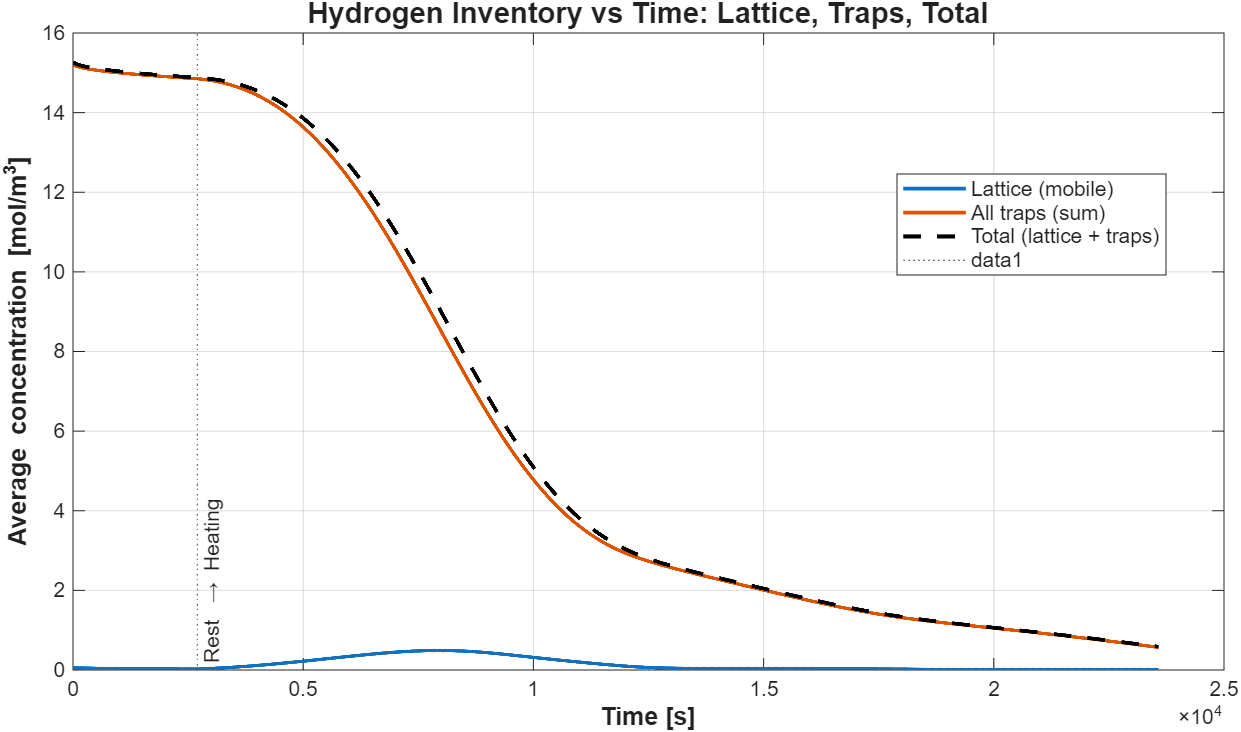
\includegraphics[width=\figwidth]{hydrogen_inventory_vs_time_baseline_study.png}
    \caption{Volume-averaged hydrogen inventory over time during the baseline simulation.}
    \label{fig:hydrogen_inventory_time}
\end{figure}

One thing that is, however, noticed is that according to Novak's experimental work, the total hydrogen in the material is reported as $1.62\text{ ppm}$, whereas the initial condition using Marrani et al.'s parameters corresponds to $1.95\text{ ppm}$ hydrogen in the sample. One reason that could explain this disparity is the 4th trap present in the sample with high binding energy ($|\Delta H_4| = 128.95\text{ kJ/mol}$), which they account for as a numerical artifact. This trap holds approximately $0.15\text{ ppm}$ hydrogen, but it still doesn't make up for the model predicting approximately 21 percent more hydrogen than it should account for.

\subsection{Comparison Between Simulation and Experimental Data}

The simulated TDS spectrum is compared directly against the digitized experimental values taken from Novak et al.~\cite{Novak2010}

\begin{figure}[htbp]
    \centering
    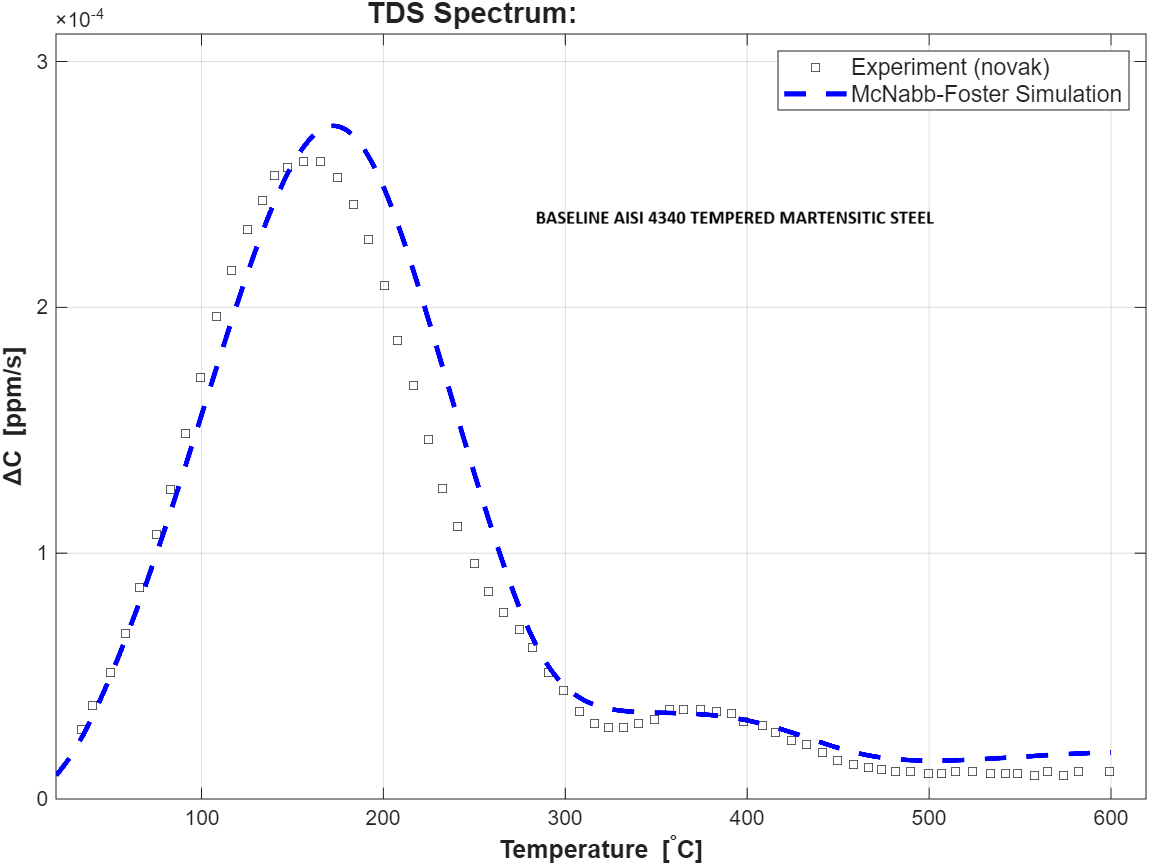
\includegraphics[width=\figwidth]{tdscurve_BASELINE.png}
    \caption{Simulated TDS spectrum compared with the experimental data of Novak et al.\ for AISI 4340 steel.}
    \label{fig:tds_baseline_comparison}
\end{figure}

The experimental spectrum exhibits a primary desorption spectrum peak centered between $155^\circ\text{C}$ and $165^\circ\text{C}$, followed by a secondary shoulder between $300^\circ\text{C}$ and $400^\circ\text{C}$. Quantitatively, the computed simulation peak is $2.73 \times 10^{-4}\text{ ppm/s}$; the digitized experimental peak is $\approx 2.6 \times 10^{-4}\text{ ppm/s}$ (approximate visual estimate). The peak height is overpredicted by $+5\%$ ($\pm 2\%$). The computed simulation peak temperature is $172.9^\circ\text{C}$; the experimental peak occurs at $\approx 155\text{--}165^\circ\text{C}$. That is an offset of $+10\text{ to } +15\text{ K}$. During the descent of the curve from the primary peak, that is from approximately $180^\circ\text{C}$ to $260^\circ\text{C}$, the simulation overestimates the desorption flux by $\approx +15\text{ to } +30\%$ relative to experimental points. In the mid-temperature shoulder range ($300\text{--}400^\circ\text{C}$), the simulation shows close agreement with the experiment at $\approx 0.35 \times 10^{-4}\text{ ppm/s}$. In the high-temperature tail ($>450^\circ\text{C}$), the simulation overpredicts flux ($0.15\text{--}0.19 \times 10^{-4}\text{ ppm/s}$ simulated vs.\ $0.10 \times 10^{-4}\text{ ppm/s}$ experimental), an absolute overestimation of $\approx +0.05\text{ to } +0.08 \times 10^{-4}\text{ ppm/s}$ ($\approx 2\text{--}3\%$ of peak height). In the low-temperature flux region ($20\text{--}40^\circ\text{C}$), the simulation underestimates the initial flux ($0.10 \times 10^{-4}\text{ ppm/s}$ simulated vs.\ $\approx 0.22 \times 10^{-4}\text{ ppm/s}$ experimental).

\begin{figure}[htbp]
    \centering
    \begin{subfigure}[b]{0.48\textwidth}
        \centering
        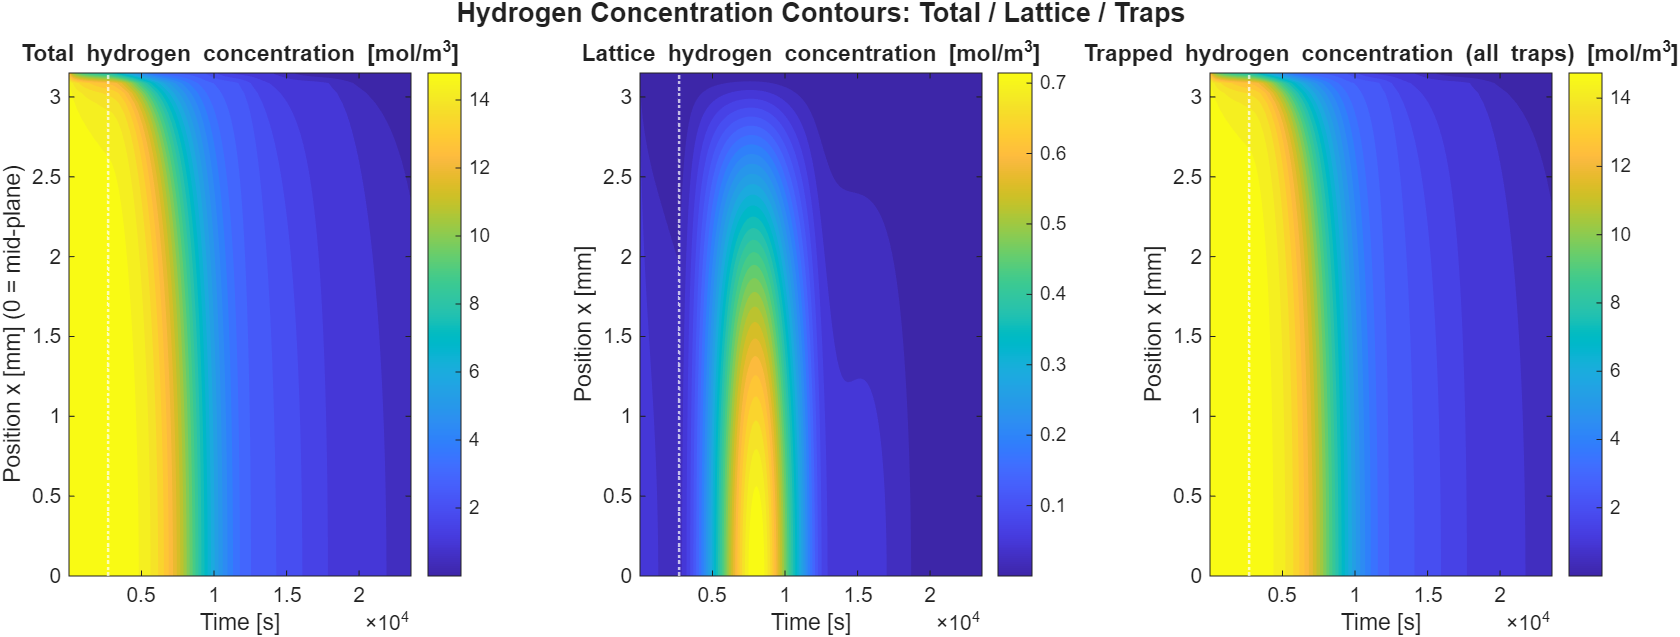
\includegraphics[width=\linewidth]{TOTAL_CONCENTRAIONS_BASELINE_STUDY.png}
        \caption{Total, lattice, and aggregate trapped concentration}
        \label{fig:contours_aggregate}
    \end{subfigure}\hfill
    \begin{subfigure}[b]{0.48\textwidth}
        \centering
        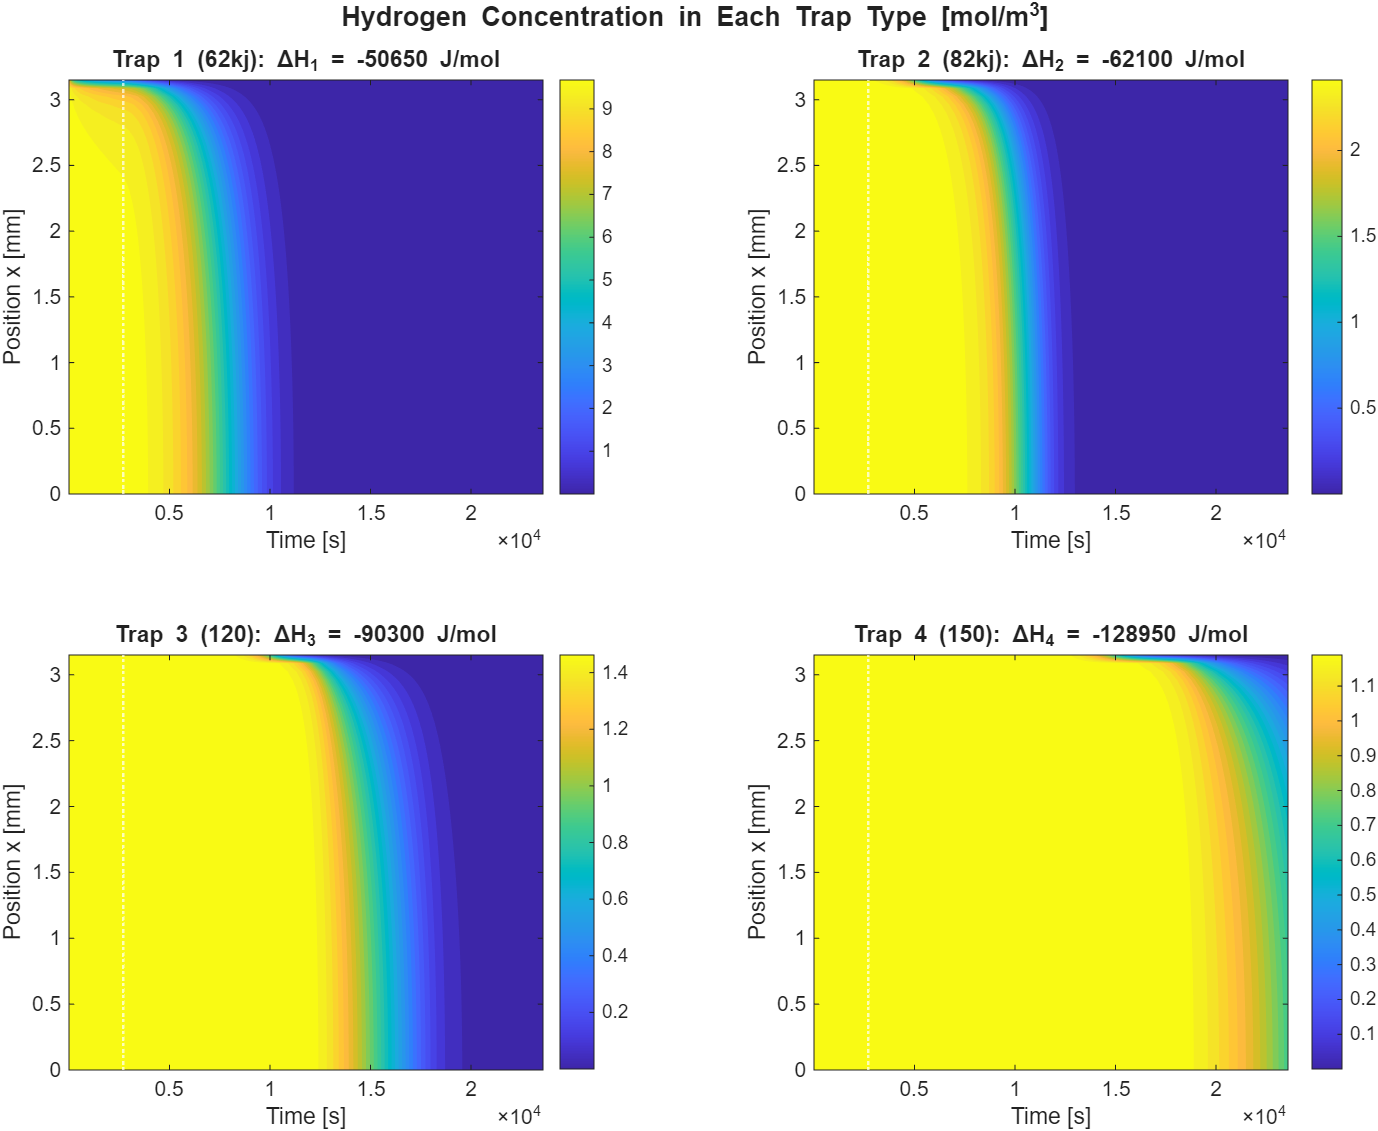
\includegraphics[width=\linewidth]{HYDROGEN_CONCENTRAION_EACH_TRAPS_BASELINE_STUDY.png}
        \caption{Concentration in individual trap populations}
        \label{fig:contours_individual}
    \end{subfigure}
    \caption{Spatiotemporal hydrogen concentration across the half-thickness during the baseline simulation.}
    \label{fig:hydrogen_concentration_contours}
\end{figure}

Desorption occurs sequentially in order of increasing trap binding energy. The trap-wise contour shows each trap emptying at different times (time and temperature have a direct linear relationship because of the constant $100\text{ K/h}$ heating rate). We can also observe the concentration gradient towards the boundary, indeed verifying that our numerical system is correctly mimicking real-world Fickian behavior of moving from a high-concentration mid-plane to a lower-concentration surface. Also, we can see that hydrogen leaves the lower binding energy traps at lower temperatures, whereas the higher binding energy traps release hydrogen at higher temperatures. The movement of hydrogen is indeed from traps to lattice concentration and then diffusing out, which is clearly visible from the contours. Correlating the concentration contours and the TDS spectra, it is thus concluded that the primary peak in the TDS spectra is associated with the lower and mid-range binding energy traps, whereas the higher binding energy traps contribute to the later part of the TDS spectra. Another observation is that even though the lower binding energy traps empty almost completely, the stronger binding energy traps retain the hydrogen in the sample; in this case, at $600^\circ\text{C}$, $3.9\%$ ($0.5843\text{ mol/m}^3$) of the initial hydrogen remains retained in the specimen, which is related exclusively to the deepest trap state ($|\Delta H_4| = 128.95\text{ kJ/mol}$).

However, there are certain limitations within this baseline study because the parameters were taken from Marrani et al.'s paper and their results, and the verification was done against Novak's experimental work; any physical errors in their work are also reflected here. So, the main purpose of this section was to reproduce the work and ensure that our numerical system is capable of getting the right parameters if given a new, independent experimental TDS spectrum along with the right parameters.

%------------------------------------------------
\section{Mesh and Time-Step Independence Study}
%------------------------------------------------

To separate numerical discretization errors from how the physical model behaves, a convergence study was done using linear finite elements in space ($n_{\mathrm{el}}$) and the Backward Euler implicit scheme in time ($\Delta t$).

\subsection{Spatial Mesh Convergence}

Mesh independence was evaluated at a constant time step of $\Delta t = 0.5\text{ s}$ across six mesh densities: $n_{\mathrm{el}} = 10, 25, 50, 100, 200,$ and $400$ elements across the half-thickness domain ($3.15\text{ mm}$). Errors were calculated relative to the finest mesh that was taken ($n_{\mathrm{el}} = 400$).

\begin{figure}[htbp]
    \centering
    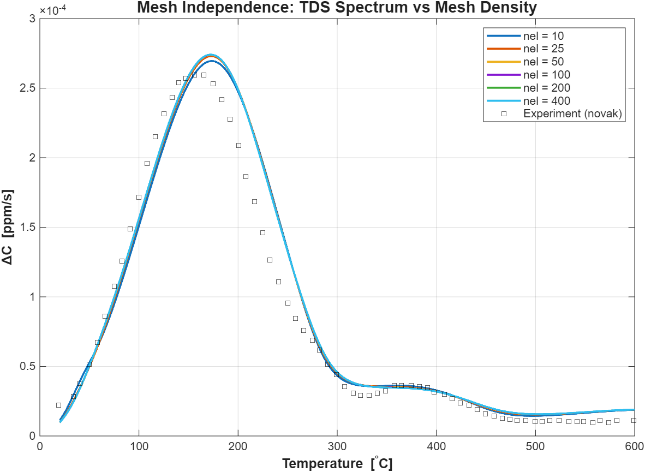
\includegraphics[width=\figwidth]{meshtds.png}
    \caption{Simulated TDS spectra for different mesh densities, which overlap for $n_{\mathrm{el}} \ge 25$.}
    \label{fig:mesh_independence_spectra}
\end{figure}

\begin{table}[htbp]
\centering
\caption{Spatial mesh convergence study}
\label{tab:mesh_convergence}
\tablestyle
\fitwidth{%
\begin{tabular}{ccccccc}
\toprule
$n_{\mathrm{el}}$ & \textbf{Peak Flux} & \textbf{Peak Temp} & \textbf{Total Released} & \textbf{Rel. Error} & \textbf{Rel. Error} & \textbf{Computation} \\
 & ($10^{-4}\text{ ppm/s}$) & ($^\circ\text{C}$) & ($\text{ppm}$) & \textbf{Peak Flux (\%)} & \textbf{Total (\%)} & \textbf{Run Time (s)} \\
\midrule
10  & $2.6945$ & $173.4$ & $1.8140$ & $1.6987\%$ & $1.3324\%$ & $215.7$ \\
25  & $2.7300$ & $172.9$ & $1.8310$ & $0.4029\%$ & $0.4050\%$ & $518.6$ \\
50  & $2.7381$ & $172.6$ & $1.8360$ & $0.1065\%$ & $0.1343\%$ & $1058.9$ \\
100 & $2.7404$ & $172.4$ & $1.8378$ & $0.0225\%$ & $0.0373\%$ & $2021.9$ \\
200 & $2.7409$ & $172.4$ & $1.8383$ & $0.0034\%$ & $0.0079\%$ & $4111.5$ \\
400 & $2.7410$ & $172.3$ & $1.8385$ & $0.0000\%$ (Ref) & $0.0000\%$ (Ref) & $8705.4$ \\
\bottomrule
\end{tabular}%
}
\end{table}

Doubling the mesh density reduced the peak flux relative error by factors of 4.2, 3.8, 4.7, and 6.6 when we double or nearly double the mesh ($10 \rightarrow 25$, $25 \rightarrow 50$, $50 \rightarrow 100$, $100 \rightarrow 200$). The log--log error plot shows the asymptotic spatial convergence rate of $1.9\text{ to } 2.2$ on coarse-to-medium meshes, confirming the theoretical $\mathcal{O}(h^2)$ second-order accuracy of linear finite elements.

\begin{figure}[htbp]
    \centering
    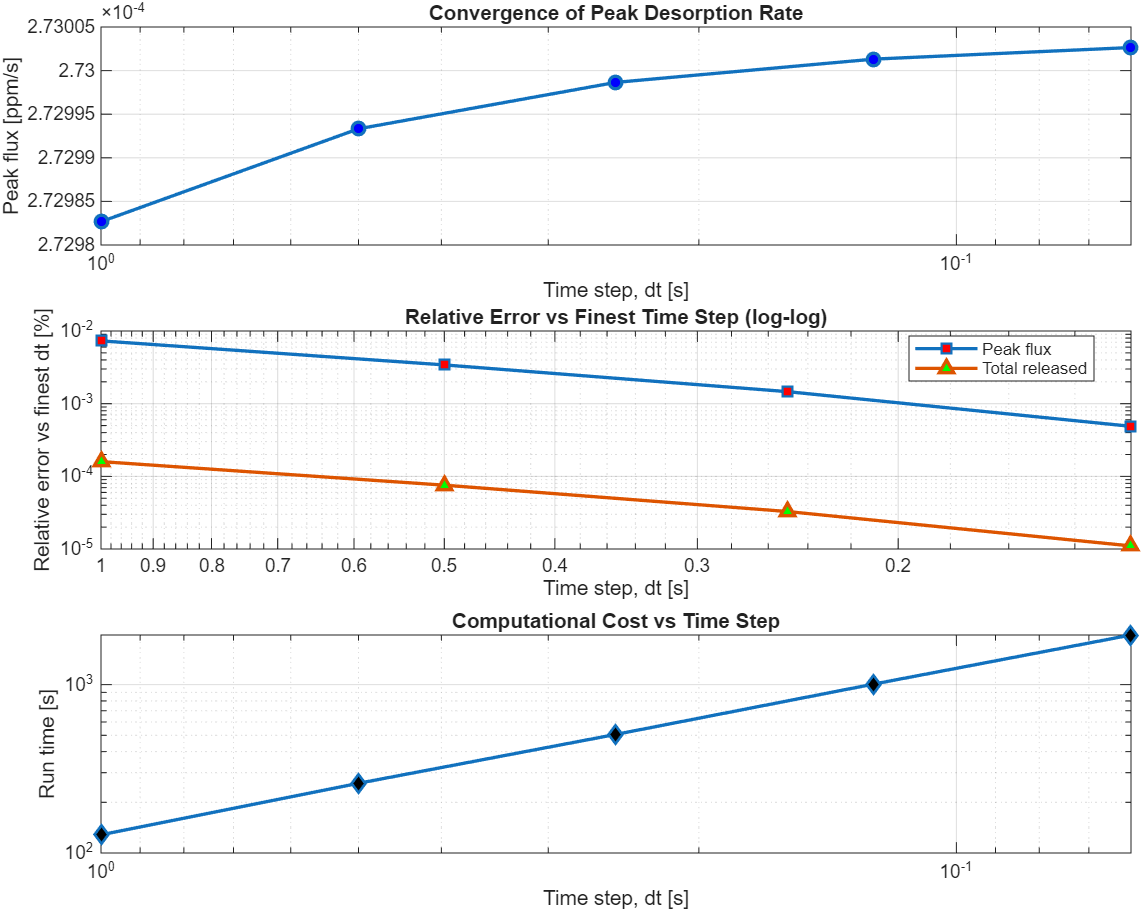
\includegraphics[width=\figwidthwide]{mesh_convergence_plot.png}
    \caption{Mesh convergence of the peak flux, relative error and computation time.}
    \label{fig:spatial_mesh_convergence}
\end{figure}

Applying second-order Richardson extrapolation ($p=2$) to the $n_{\mathrm{el}} = 100$ and $200$ solutions gives an estimated continuum-limit peak flux of $2.741 \times 10^{-4}\text{ ppm/s}$, identical to the $n_{\mathrm{el}} = 400$ solution. Also, the peak temperature shifts by only $1.1\text{ K}$ across the entire mesh range ($173.4^\circ\text{C}$ at $n_{\mathrm{el}}=10$ vs.\ $172.3^\circ\text{C}$ at $n_{\mathrm{el}}=400$).

The computational run time varies linearly with the element count ($\mathcal{O}(n_{\mathrm{el}})$), increasing from $215.7\text{ s}$ ($n_{\mathrm{el}}=10$) to $8705.4\text{ s}$ ($n_{\mathrm{el}}=400$). Refinement beyond $n_{\mathrm{el}} = 50$ increases CPU time by $800\%$ while giving only a $< 0.11\%$ gain in accuracy.

These results provide evidence that the spatial discretization error is small. Also, since we are required to generate a large number of datasets for training, choosing $n_{\mathrm{el}} = 25$ seems to be the better option when considering the computational cost; however, the initial parameter study is done by taking $n_{\mathrm{el}} = 50$.

\subsection{Time-Step Convergence Study}

Time-step independence was evaluated on a fixed mesh of $n_{\mathrm{el}} = 25$ across five time steps: $\Delta t = 1.0, 0.5, 0.25, 0.125,$ and $0.0625\text{ s}$. Errors were referenced to the $\Delta t = 0.0625\text{ s}$ solution.

\begin{figure}[htbp]
    \centering
    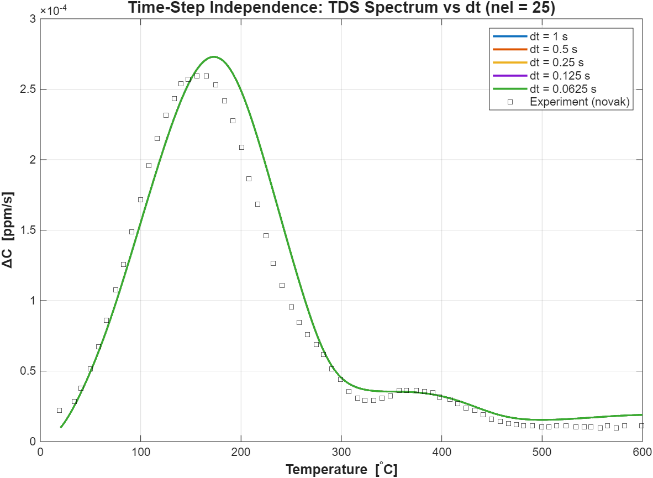
\includegraphics[width=\figwidth]{timetds.png}
    \caption{Simulated TDS spectra for time steps from $1.0\text{ s}$ to $0.0625\text{ s}$ on a fixed mesh of $n_{\mathrm{el}} = 25$.}
    \label{fig:time_step_independence}
\end{figure}

\begin{table}[htbp]
\centering
\caption{Time-step convergence study}
\label{tab:time_convergence}
\tablestyle
\fitwidth{%
\begin{tabular}{ccccccc}
\toprule
$\Delta t$ (\text{s}) & \textbf{Peak Flux} & \textbf{Peak Temp} & \textbf{Total Released} & \textbf{Rel. Error} & \textbf{Rel. Error} & \textbf{Computation} \\
 & ($10^{-4}\text{ ppm/s}$) & ($^\circ\text{C}$) & ($\text{ppm}$) & \textbf{Peak Flux (\%)} & \textbf{Total (\%)} & \textbf{Run Time (s)} \\
\midrule
1.000  & $2.7298$ & $172.9$ & $1.8310$ & $0.0073\%$ & $1.59 \times 10^{-4}\%$ & $128.3$ \\
0.500  & $2.7299$ & $172.9$ & $1.8310$ & $0.0034\%$ & $7.56 \times 10^{-5}\%$ & $259.5$ \\
0.250  & $2.7300$ & $172.9$ & $1.8310$ & $0.0015\%$ & $3.28 \times 10^{-5}\%$ & $506.5$ \\
0.125  & $2.7300$ & $172.9$ & $1.8310$ & $0.0005\%$ & $1.10 \times 10^{-5}\%$ & $1007.2$ \\
0.0625 & $2.7300$ & $172.9$ & $1.8310$ & $0.0000\%$ (Ref) & $0.0000\%$ (Ref) & $1971.7$ \\
\bottomrule
\end{tabular}%
}
\end{table}

Halving the time step reduces peak flux error by factors of $2.1$, $2.3$, and $3.0$, corresponding to an observed temporal convergence order of $1.1\text{ to } 1.6$, consistent with the theoretical $\mathcal{O}(\Delta t)$ first-order accuracy of Backward Euler. Also, at $n_{\mathrm{el}} = 25$, the temporal discretization error ($0.0034\%$ at $\Delta t = 0.5\text{ s}$) is 2 to 3 orders of magnitude smaller than the spatial mesh error ($0.4029\%$). The peak temperature remains identical at $172.9^\circ\text{C}$ for all tested time steps.

\begin{figure}[htbp]
    \centering
    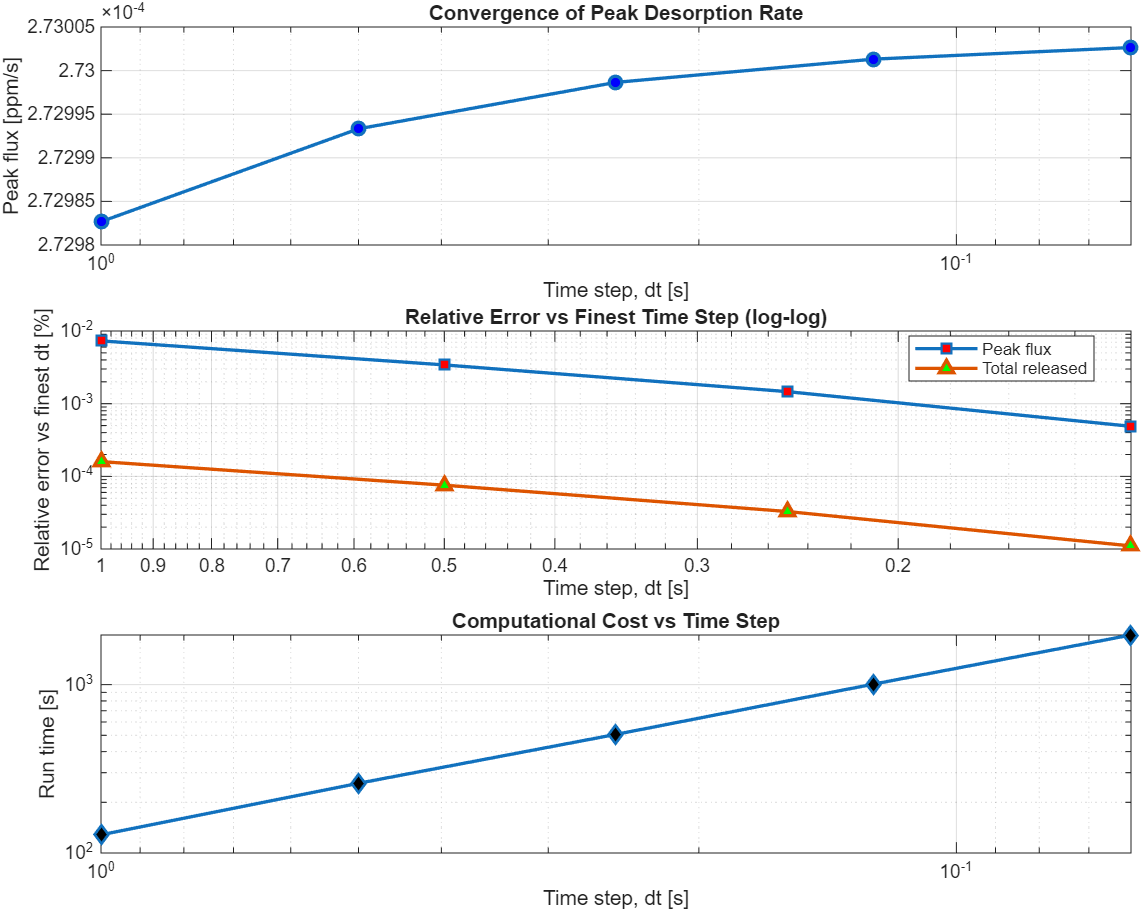
\includegraphics[width=\figwidthwide]{time_convergence_plot.png}
    \caption{Convergence of the simulated TDS response as the time step is reduced.}
    \label{fig:time_step_independence_plot}
\end{figure}

Since the error associated with spatial discretization is orders of magnitude higher than temporal discretization, we can say that it is temporally over-resolved. However, we will be keeping $0.5\text{ s}$ as a conservative choice in our further data generation process. Theoretically, changing both simultaneously could have effects that aren't visible when studying them separately, but this possible interaction between mesh and time step was not examined. Since spatial error is dominating, even if there is some interaction, it is unlikely to change the obtained results.

%------------------------------------------------
\section{Parametric Sensitivity Analysis}
%------------------------------------------------

Following the numerical study, a sensitivity analysis was performed to identify which parameters exert the greatest influence on the simulated TDS curve. The analysis considered material parameters, trap characteristics, specimen geometry, boundary-condition parameters, and experimental conditions. Three response quantities were used repeatedly to quantify the effect of each parameter:
\begin{align}
J_{\max} &= \max_T J(T) \\
T_{\mathrm{peak}} &= \arg\max_T J(T) \\
H_{\mathrm{des}} &= \int J(t)\,dt
\end{align}

\subsection{Effect of Binding Energy}

Increasing the binding energy caused the peak temperature to increase strictly linearly across the interior range ($50\text{--}130\text{ kJ/mol}$) with a slope of $+5.96\text{ K per kJ/mol}$ ($T_{\mathrm{p}} \approx 92.8 + 5.96(|\Delta H|-50)^\circ\text{C}$). This linear relationship arises because detrapping is an Arrhenius-activated process with barrier $E_{\mathrm{d}} = E_{\mathrm{L}} + |\Delta H|$. At a constant heating rate, peak release occurs where $E_{\mathrm{d}} / (R T_{\mathrm{p}}) \approx 18\text{--}19$, making $T_{\mathrm{p}}$ directly proportional to $E_{\mathrm{d}}$.

\begin{figure}[htbp]
    \centering
    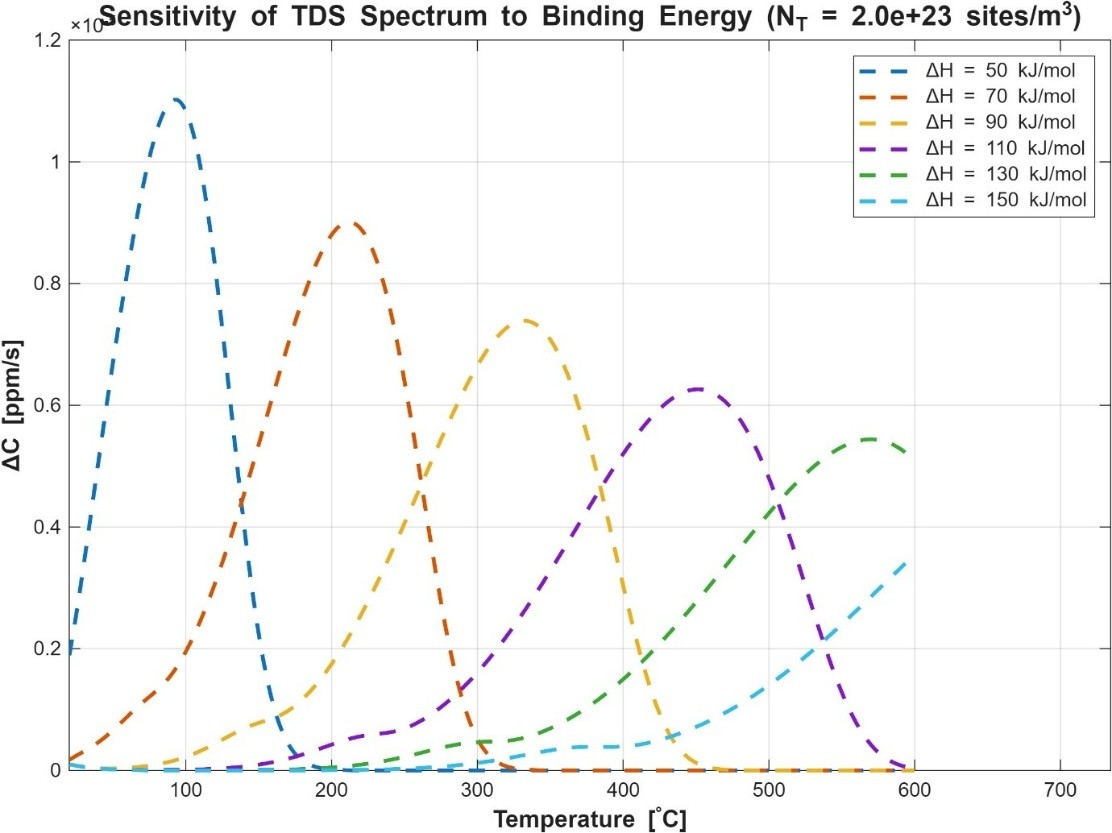
\includegraphics[width=\figwidth]{binding_tds.jpg}
    \caption{Effect of trap binding energy on the simulated TDS spectrum for a single trap of $2.0 \times 10^{23}\text{ sites/m}^3$.}
    \label{fig:sensitivity_binding_energy}
\end{figure}

The peak height falls monotonically ($18\%, 33\%, 43\%, 51\%$ drop relative to $50\text{ kJ/mol}$). Normalized arc sensitivities between $70$ and $90\text{ kJ/mol}$ are $S_J \approx -0.79$ and $S_T \approx +0.88$. Since higher binding energy broadens the desorption curve, in order to conserve the total amount of hydrogen (that is, the area under the curve), the peak height must drop. The anomalous drop in $H_{\mathrm{des}}$ at $130$ and $150\text{ kJ/mol}$ is a consequence of truncation at $600^\circ\text{C}$ ($24.6\%$ and $70.0\%$ retained), not of weaker trapping. During the $2700\text{ s}$ room-temperature rest hold prior to heating at $50\text{ kJ/mol}$, $17\%$ of trapped hydrogen escapes, thus reducing the total desorbed hydrogen.

\begin{figure}[htbp]
    \centering
    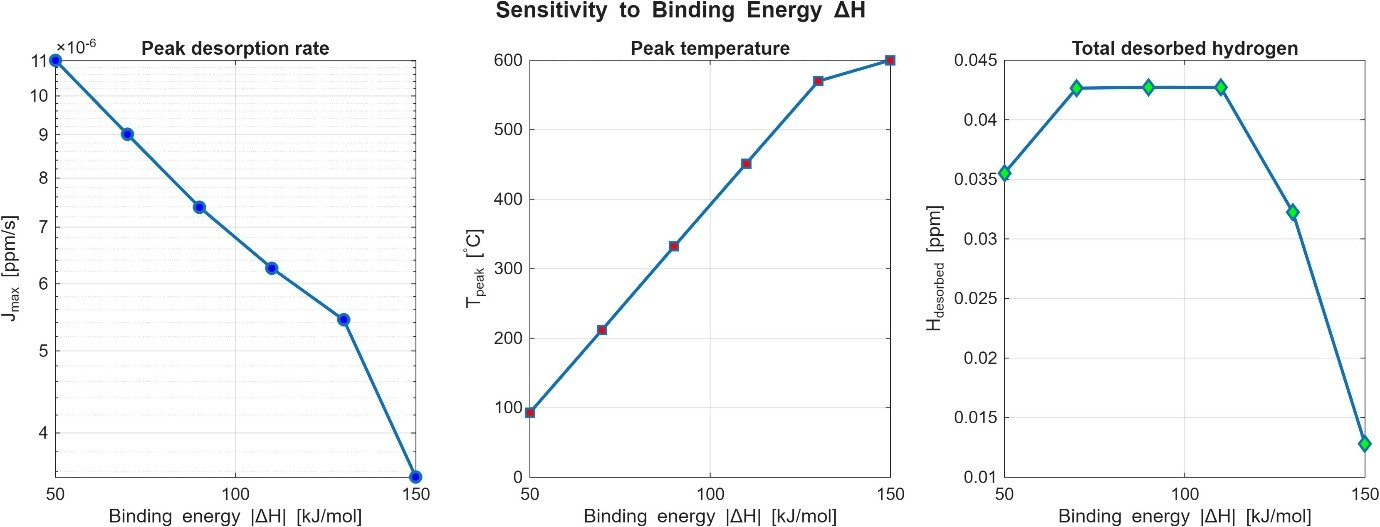
\includegraphics[width=\figwidthwide]{bindingconv.jpg}
    \caption{Variation of peak flux, peak temperature and total desorbed hydrogen with trap binding energy.}
    \label{fig:sensitivity_metrics_binding_energy}
\end{figure}

\subsection{Effect of Trap Density (\texorpdfstring{$N_{\mathrm{T}}$}{N\_T})}

Trap density was varied from $10^{19}$ to $10^{24}\text{ sites/m}^3$ for a single trap ($|\Delta H| \approx 80\text{ kJ/mol}$).

\begin{table}[htbp]
\centering
\caption{Effect of Trap Density on TDS Response}
\label{tab:trap_density}
\tablestyle
\fitwidth{%
\begin{tabular}{ccccccc}
\toprule
$N_{\mathrm{T}}$ & $N_{\mathrm{T}}$ & $J_{\max}$ & $T_{\mathrm{p}}$ & $H_{\mathrm{des}}$ & $H_{\mathrm{start}}$ & $H_{\mathrm{final}}$ \\
($\text{sites/m}^3$) & ($\text{mol/m}^3$) & ($\text{ppm/s}$) & ($^\circ\text{C}$) & ($\text{ppm}$) & ($\text{mol/m}^3$) & ($\text{mol/m}^3$) \\
\midrule
$10^{19}$ & $1.661 \times 10^{-5}$ & $1.0079 \times 10^{-7}$ & $20.06$ & $6.0296 \times 10^{-5}$ & $4.708 \times 10^{-4}$ & $2.83 \times 10^{-50}$ \\
$10^{20}$ & $1.661 \times 10^{-4}$ & $1.0079 \times 10^{-7}$ & $20.06$ & $7.9494 \times 10^{-5}$ & $6.202 \times 10^{-4}$ & $3.32 \times 10^{-47}$ \\
$10^{21}$ & $1.661 \times 10^{-3}$ & $1.0082 \times 10^{-7}$ & $20.06$ & $2.7147 \times 10^{-4}$ & $2.115 \times 10^{-3}$ & $5.39 \times 10^{-43}$ \\
$10^{22}$ & $1.661 \times 10^{-2}$ & $5.1625 \times 10^{-7}$ & $204.83$ & $2.1912 \times 10^{-3}$ & $1.706 \times 10^{-2}$ & $3.70 \times 10^{-37}$ \\
$10^{23}$ & $1.661 \times 10^{-1}$ & $4.3065 \times 10^{-6}$ & $254.94$ & $2.1388 \times 10^{-2}$ & $1.665 \times 10^{-1}$ & $9.27 \times 10^{-29}$ \\
$10^{24}$ & $1.661 \times 10^{0}$ & $3.5119 \times 10^{-5}$ & $316.06$ & $2.1336 \times 10^{-1}$ & $1.661 \times 10^{0}$ & $6.78 \times 10^{-17}$ \\
\bottomrule
\end{tabular}%
}
\end{table}

The maximum desorption rate remains constant at $J \approx 1.008 \times 10^{-7}\text{ ppm/s}$ at $20.06^\circ\text{C}$ for $N_{\mathrm{T}} \le 10^{21}\text{ sites/m}^3$. The flat curve represents the mobile lattice hydrogen that is in the material, not from a trap release peak. For $N_{\mathrm{T}} \ge 10^{22}\text{ sites/m}^3$, the peak flux increases almost linearly with trap density following $J_{\max} \propto N_{\mathrm{T}}^{0.91\text{--}0.92}$ ($8.34\times$ and $8.15\times$ increase per decade). Whereas the total released hydrogen follows an exact stoichiometry: $H_{\mathrm{des}} \approx 0.1284 N_{\mathrm{T}}\text{ [mol/m}^3\text{] ppm}$.

The peak temperature shifts upwards by $+50\text{ K}$ and $+61\text{ K}$ per decade (total shift of $+111\text{ K}$ from $10^{22}$ to $10^{24}\text{ sites/m}^3$). If the process was purely a detrapping-limited process, $T_{\mathrm{p}}$ would have been independent of trap density; however, this large positive shift confirms that desorption in thick specimens is diffusion-limited with retrapping reaching the surface. This confirms that the classic Kissinger kinetic analysis fails for non-thin TDS specimens.

\begin{figure}[htbp]
    \centering
    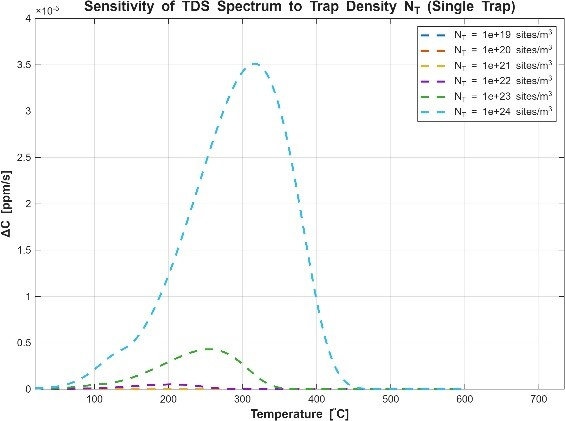
\includegraphics[width=\figwidth]{traptds.jpg}
    \caption{Effect of trap density on the simulated TDS spectrum for a single trap population.}
    \label{fig:sensitivity_trap_density}
\end{figure}

\begin{figure}[htbp]
    \centering
    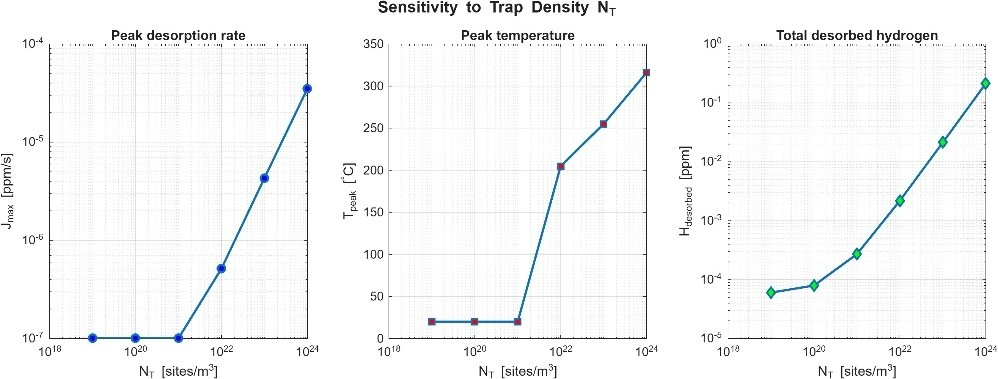
\includegraphics[width=\figwidthwide]{trapconv.jpg}
    \caption{Variation of peak flux, peak temperature and total desorbed hydrogen with trap density.}
    \label{fig:sensitivity_metrics_trap_density}
\end{figure}

\subsection{Effect of Initial Lattice Concentration (\texorpdfstring{$C_{L,0}$}{C\_L0})}

Initial lattice concentration was varied over a 100-fold range ($0.006$ to $0.600\text{ mol/m}^3$) around the baseline value ($0.06\text{ mol/m}^3$).

\begin{table}[htbp]
\centering
\caption{Effect of Initial Lattice Concentration}
\label{tab:initial_conc}
\tablestyle
\fitwidth{%
\begin{tabular}{cccccccc}
\toprule
$C_{L,0}$ & \textbf{Scaling} & $J_{\max}$ & $\Delta J_{\max}$ & $T_{\mathrm{p}}$ & $\Delta T_{\mathrm{p}}$ & $H_{\mathrm{des}}$ & $\Delta H_{\mathrm{des}}$ \\
($\text{mol/m}^3$) & \textbf{Factor} & ($10^{-4}\text{ ppm/s}$) & ($\%$) & ($^\circ\text{C}$) & ($\text{K}$) & ($\text{ppm}$) & ($\%$) \\
\midrule
0.006 & $0.1\times$ & $2.6497$ & $-2.9\%$ & $175.61$ & $+2.72\text{ K}$ & $1.712$ & $-6.5\%$ \\
0.045 & $0.75\times$ & $2.7285$ & $-0.1\%$ & $172.94$ & $+0.06\text{ K}$ & $1.827$ & $-0.2\%$ \\
0.060 & $1.0\times$ (Base) & $2.7299$ & $0.0\%$ & $172.89$ & $0.00\text{ K}$ & $1.831$ & $0.0\%$ \\
0.075 & $1.25\times$ & $2.7307$ & $+0.0\%$ & $172.89$ & $0.00\text{ K}$ & $1.834$ & $+0.1\%$ \\
0.600 & $10.0\times$ & $2.7350$ & $+0.2\%$ & $172.72$ & $-0.17\text{ K}$ & $1.851$ & $+1.1\%$ \\
\bottomrule
\end{tabular}%
}
\end{table}

\begin{figure}[htbp]
    \centering
    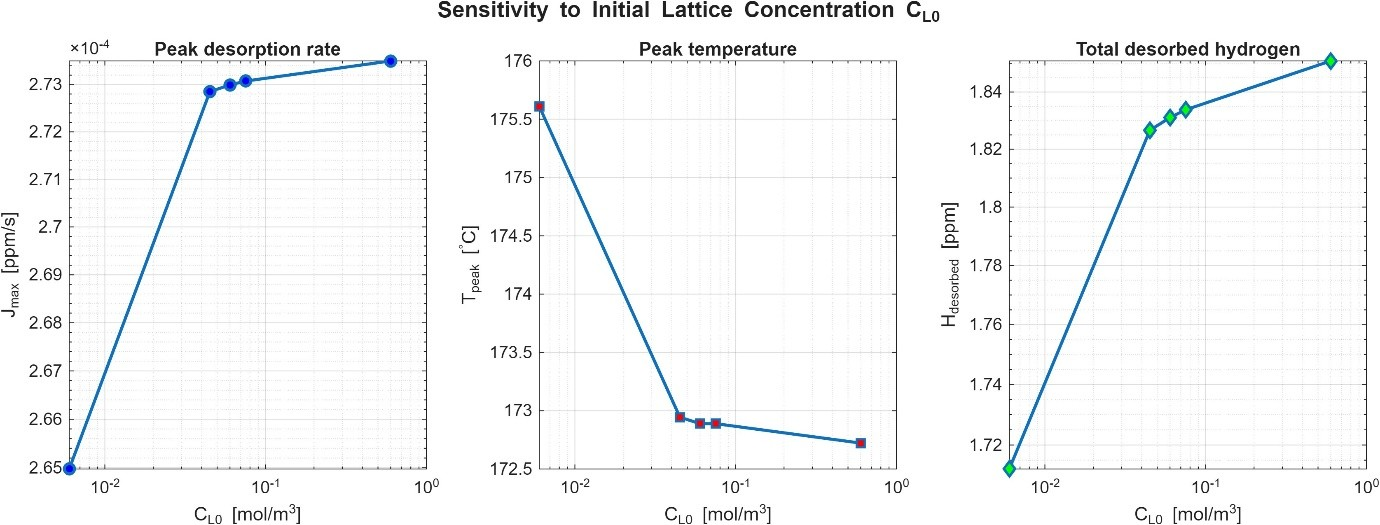
\includegraphics[width=\figwidthwide]{initialconcconv.jpg}
    \caption{Variation of peak flux, peak temperature and total desorbed hydrogen with initial lattice concentration.}
    \label{fig:sensitivity_metrics_initial_conc}
\end{figure}

It is seen that even varying $C_{L,0}$ by $10000\%$ (a factor of 100) produces negligible change in peak flux ($-2.9\%$ to $+0.2\%$) and peak temperature ($+2.72\text{ K}$ to $-0.17\text{ K}$). Because initial trap occupancies are set by thermodynamic equilibrium ($\theta_{\mathrm{T,1}} \approx 0.987$ at $C_{L,0} = 0.06\text{ mol/m}^3$), deep traps are virtually saturated. Higher $C_{L,0}$ cannot increase trap occupancy above $100\%$. Mobile lattice hydrogen represents only $0.4\%$ of the total inventory and desorbs immediately during rest. Thus, we can say that the initial lattice concentration doesn't affect the TDS spectra that largely. If we know the charging pressure, even as an approximation, as long as it is in the same order of magnitude, it will not affect the simulations significantly. However, it is to be noted that the total hydrogen content does depend on the initial concentration and that conservation laws must be satisfied. We can see the discrepancy there in the baseline model, where the experimental data shows approximately $1.62\text{ ppm}$, whereas our initial equilibrium condition caused it to be around $1.95\text{ ppm}$.

\begin{figure}[htbp]
    \centering
    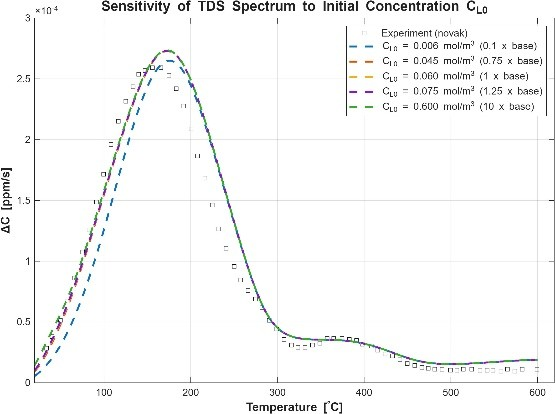
\includegraphics[width=\figwidth]{initialconctds.jpg}
    \caption{Effect of the initial lattice concentration on the simulated TDS spectrum.}
    \label{fig:sensitivity_initial_conc_spectrum}
\end{figure}

\subsection{Effect of Lattice Diffusivity (\texorpdfstring{$D_0$ and $E_{\mathrm{L}}$}{D0 and E\_L})}

Both parameters act only through $D_{\mathrm{L}} = D_0 \exp(-E_{\mathrm{L}}/RT)$, but they do so differently and are analyzed separately.

\begin{table}[htbp]
\centering
\caption{Effect of Lattice Diffusivity Parameters}
\label{tab:diffusivity}
\tablestyle
\fitwidth{%
\begin{tabular}{lcccccc}
\toprule
\textbf{Parameter Change} & \textbf{Parameter Value} & $J_{\max}$ & $\Delta J_{\max}$ & $T_{\mathrm{p}}$ & $\Delta T_{\mathrm{p}}$ & $H_{\mathrm{des}}$ \\
 & & ($10^{-4}\text{ ppm/s}$) & ($\%$) & ($^\circ\text{C}$) & ($\text{K}$) & ($\text{ppm}$) \\
\midrule
$D_0 \times 0.1$ & $7.23 \times 10^{-9}\text{ m}^2/\text{s}$ & $1.7460$ & $-36.04\%$ & $260.06$ & $+87.17\text{ K}$ & $1.7649$ \\
$D_0 \times 0.75$ & $5.42 \times 10^{-8}\text{ m}^2/\text{s}$ & $2.6266$ & $-3.78\%$ & $181.72$ & $+8.83\text{ K}$ & $1.8274$ \\
$D_0 \times 1.0$ (Base) & $7.23 \times 10^{-8}\text{ m}^2/\text{s}$ & $2.7299$ & $0.00\%$ & $172.89$ & $0.00\text{ K}$ & $1.8310$ \\
$D_0 \times 1.25$ & $9.04 \times 10^{-8}\text{ m}^2/\text{s}$ & $2.8086$ & $+2.88\%$ & $166.44$ & $-6.45\text{ K}$ & $1.8334$ \\
$D_0 \times 10.0$ & $7.23 \times 10^{-7}\text{ m}^2/\text{s}$ & $3.5402$ & $+29.68\%$ & $117.17$ & $-55.72\text{ K}$ & $1.8162$ \\
\midrule
$E_{\mathrm{L}} \times 0.5$ & $2.845\text{ kJ/mol}$ & $2.8809$ & $+5.53\%$ & $148.78$ & $-24.11\text{ K}$ & $1.8130$ \\
$E_{\mathrm{L}} \times 0.75$ & $4.268\text{ kJ/mol}$ & $2.8047$ & $+2.74\%$ & $160.61$ & $-12.28\text{ K}$ & $1.8240$ \\
$E_{\mathrm{L}} \times 1.25$ & $7.112\text{ kJ/mol}$ & $2.6554$ & $-2.73\%$ & $185.78$ & $+12.89\text{ K}$ & $1.8350$ \\
$E_{\mathrm{L}} \times 1.5$ & $8.535\text{ kJ/mol}$ & $2.5797$ & $-5.50\%$ & $199.39$ & $+26.50\text{ K}$ & $1.8350$ \\
\bottomrule
\end{tabular}%
}
\end{table}

The peak temperature is found to shift by $\approx 30\text{ K}$ per ln-unit change in $D_0$ ($28.9$ and $30.7\text{ K/ln-unit}$ for $\pm 25\%$), whereas the peak temperature is found to shift linearly by $+8.5\text{ to } +9.3\text{ K per kJ/mol}$ of migration energy. If we fix $T_{\mathrm{p}} \approx 446\text{ K}$, a $1\text{ kJ/mol}$ shift in $E_{\mathrm{L}}$ alters $\ln D_{\mathrm{L}}$ by $\frac{1000}{R T_{\mathrm{p}}} = 0.27\text{ ln-units}$. If we multiply this $0.27$ by the $D_0$ sensitivity ($30\text{ K/ln-unit}$), it predicts a shift of $8.1\text{ K/ (kJ/mol)}$, which agrees closely with the observed $8.5\text{--}9.3\text{ K/ (kJ/mol)}$. This shows that $D_0$ and $E_{\mathrm{L}}$ act strictly through the single coupled property $D_{\mathrm{L}}(T_{\mathrm{p}})$ effective diffusivity, making them difficult to resolve as separate parameters.

\subsection{Effect of Penalty Boundary Condition Parameters (\texorpdfstring{$k_{\mathrm{pen}}$ and $E_{\mathrm{bc}}$}{k\_pen and E\_bc})}

Hydrogen leaving the specimen is modeled using a Robin boundary condition where the surface flux is proportional to lattice hydrogen concentration. To keep the mesh coarse for faster computation, this is adopted also to replicate the near-sink condition at a surface interacting with a vacuum. The penalty boundary conditions are chosen in this way in order to scale with temperature. Thus, the hydrogen flux leaving the surface is:
\begin{equation}
j = k_{\mathrm{pen}} \theta_{\mathrm{L}} \exp\left(-\frac{E_{\mathrm{bc}}}{RT}\right)
\end{equation}
Where $k_{\mathrm{pen}}$ is the penalty/surface coefficient, and $E_{\mathrm{bc}}$ is the analogous activation energy associated with this boundary expression. This can be rewritten as:
\begin{equation}
j = b(T)\, C_{\mathrm{L}}
\end{equation}
Where the desorption boundary flux is controlled by the transfer coefficient $b(T) = \frac{k_{\mathrm{pen}}}{N_{\mathrm{L}}} \exp\left(-\frac{E_{\mathrm{bc}}}{RT}\right)$, defining the mass-transfer Biot number $\mathrm{Bi} = \frac{b(T)\, (L/2)}{D_{\mathrm{L}}}$. A high Biot number is preferred in all regimes so that the Robin condition approximately behaves like a Dirichlet boundary condition ($C_{\mathrm{L}} = 0$) at the surface.

\begin{figure}[htbp]
    \centering
    \begin{subfigure}[b]{0.48\textwidth}
        \centering
        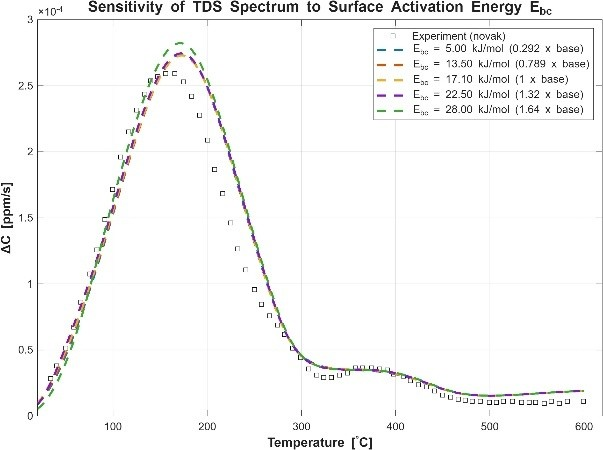
\includegraphics[width=\linewidth]{ebctds.jpg}
        \caption{Surface activation energy $E_{\mathrm{bc}}$}
        \label{fig:sensitivity_ebc}
    \end{subfigure}\hfill
    \begin{subfigure}[b]{0.48\textwidth}
        \centering
        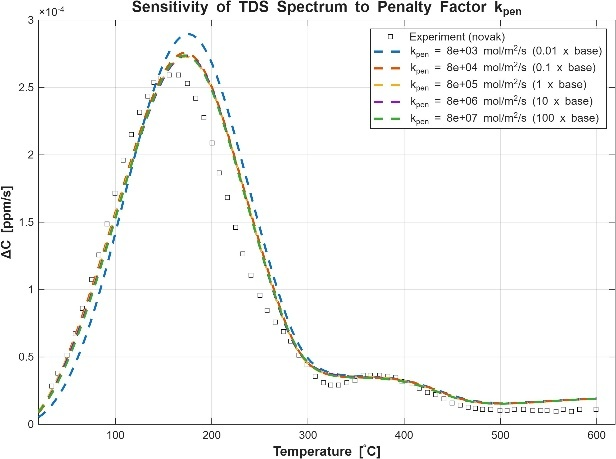
\includegraphics[width=\linewidth]{kpentds.png}
        \caption{Penalty factor $k_{\mathrm{pen}}$}
        \label{fig:sensitivity_kpen}
    \end{subfigure}
    \caption{Effect of the boundary-condition parameters on the simulated TDS spectrum.}
    \label{fig:sensitivity_bc_pair}
\end{figure}

\begin{table}[htbp]
\centering
\caption{Effect of Boundary Condition Parameters}
\label{tab:boundary_conditions}
\tablestyle
\fitwidth{%
\begin{tabular}{lcccccc}
\toprule
\textbf{Parameter Change} & \textbf{Value} & $J_{\max}$ & $\Delta J_{\max}$ & $\Delta T_{\mathrm{p}}$ & $H_{\mathrm{des}}$ & \textbf{Mid-Plane} \\
 & & ($10^{-4}\text{ ppm/s}$) & ($\%$) & ($\text{K}$) & ($\text{ppm}$) & \textbf{Biot No.} \\
\midrule
$k_{\mathrm{pen}} \times 0.01$ & $8 \times 10^3\text{ mol/m}^2/\text{s}$ & $2.8955$ & $+6.1\%$ & $+2.72\text{ K}$ & $1.867$ & $\approx 19$ (Peak) \\
$k_{\mathrm{pen}} \times 0.1$ & $8 \times 10^4\text{ mol/m}^2/\text{s}$ & $2.7565$ & $+1.0\%$ & $-0.50\text{ K}$ & $1.849$ & $\approx 190$ (Peak) \\
$k_{\mathrm{pen}} \times 1.0$ (Base) & $8 \times 10^5\text{ mol/m}^2/\text{s}$ & $2.7299$ & $0.0\%$ & $0.00\text{ K}$ & $1.831$ & $\approx 1900$ (Peak) \\
$k_{\mathrm{pen}} \times 10.0$ & $8 \times 10^6\text{ mol/m}^2/\text{s}$ & $2.7369$ & $+0.3\%$ & $+0.56\text{ K}$ & $1.823$ & $\approx 19000$ (Peak) \\
$k_{\mathrm{pen}} \times 100.0$ & $8 \times 10^7\text{ mol/m}^2/\text{s}$ & $2.7373$ & $+0.3\%$ & $-0.67\text{ K}$ & $1.819$ & $\approx 190000$ (Peak) \\
\midrule
$E_{\mathrm{bc}} = 5.0\text{ kJ/mol}$ & $0.292\times\text{Base}$ & $2.7392$ & $+0.3\%$ & $+0.11\text{ K}$ & $1.818$ & High ($\mathrm{Bi} \gg 100$) \\
$E_{\mathrm{bc}} = 22.5\text{ kJ/mol}$ & $1.32\times\text{Base}$ & $2.7448$ & $+0.5\%$ & $-0.50\text{ K}$ & $1.848$ & High ($\mathrm{Bi} \gg 100$) \\
$E_{\mathrm{bc}} = 28.0\text{ kJ/mol}$ & $1.64\times\text{Base}$ & $2.8225$ & $+3.4\%$ & $-1.61\text{ K}$ & $1.867$ & $\approx 100$ (Peak) \\
\bottomrule
\end{tabular}%
}
\end{table}

For baseline conditions, $\mathrm{Bi} \approx 380$ at $293\text{ K}$, $\approx 1900$ at peak temperature ($446\text{ K}$), and $\approx 8500$ at $873\text{ K}$. Because $\mathrm{Bi} \gg 1$, the surface resistance is negligible, and the Robin condition accurately enforces a Dirichlet state ($\theta_{\mathrm{L}} \approx 0$).

Reducing $k_{\mathrm{pen}}$ by $100\times$ drops $\mathrm{Bi}$ to $\approx 19$ at peak temperature, causing surface resistance to delay desorption ($+6.1\%$ flux rise, $+2.72\text{ K}$ thermal shift), but it is still well over 1. For all cases where $\mathrm{Bi} \ge 100$, peak flux changes are found to be $< 0.3\%$ and peak temperature shifts by $< 0.6\text{ K}$, which lies within numerical discretization error ($0.40\%$ at $n_{\mathrm{el}}=25$).

Raising $E_{\mathrm{bc}}$ to $28\text{ kJ/mol}$ reduces $b$ by a factor of $0.011$ at $293\text{ K}$, but only by about $0.05$ at $450\text{ K}$. However, $E_{\mathrm{bc}}$ still ensures that the Biot number scales with temperature as intended. Thus, it can be observed that for $\mathrm{Bi} \gtrsim 100$, the values are converged, and fixing a sufficiently high value does not affect the solution significantly.

\subsection{Effect of Specimen Thickness (\texorpdfstring{$L$}{L})}

Thickness was varied across four orders of magnitude ($0.063$ to $630\text{ mm}$) around the baseline ($6.3\text{ mm}$).

From the TDS spectra, multiple peaks were observed for thinner samples, implicating that as thickness increases, diffusion becomes more dominant over trapping-detrapping kinetics. So, in thinner samples, the multiple peaks correspond to hydrogen leaving from multiple traps, whereas in thicker specimens, the spectra have broader peaks. There is also a peak recognized at $71^\circ\text{C}$ for the highest thickness (that is $L = 630\text{ mm}$); it is an artifact of peak finding because the slope is zero at that point and can be excluded from the trends.

\begin{figure}[htbp]
    \centering
    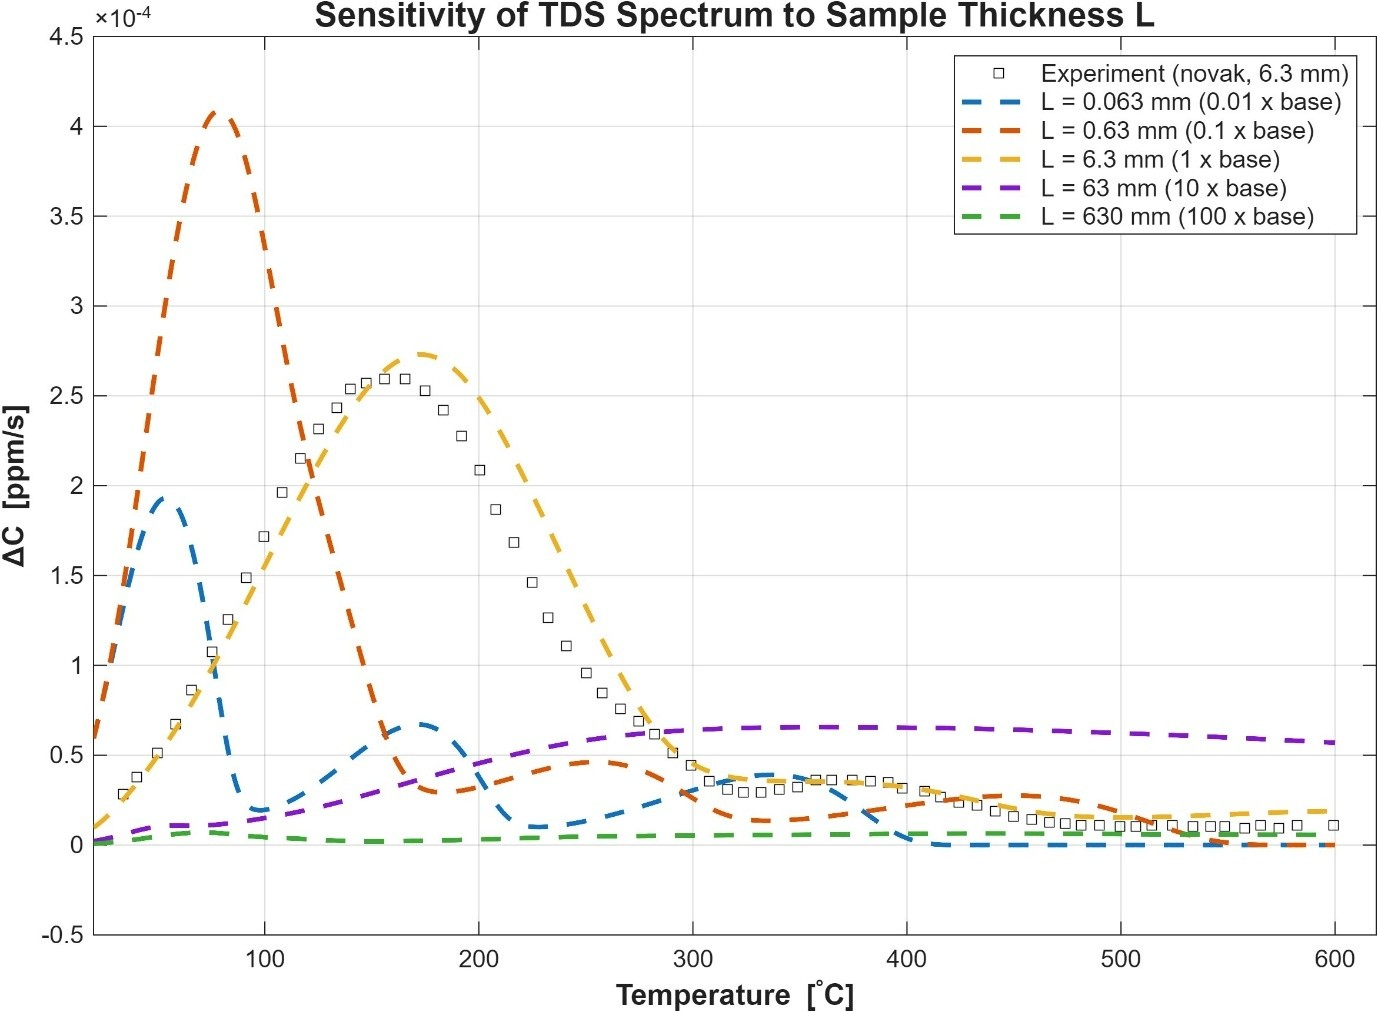
\includegraphics[width=\figwidth]{thicknesstds.jpg}
    \caption{Effect of specimen thickness on the simulated TDS spectrum.}
    \label{fig:sensitivity_thickness}
\end{figure}

\begin{table}[htbp]
\centering
\caption{Effect of Specimen Thickness on TDS Response}
\label{tab:thickness}
\tablestyle
\fitwidth{%
\begin{tabular}{lccccl}
\toprule
\textbf{Thickness $L$} & $J_{\max}$ & $T_{\mathrm{p}}$ & $H_{\mathrm{des}}$ & $H_{\mathrm{start}}$ & \textbf{Kinetic Desorption} \\
($\text{mm}$) & ($10^{-4}\text{ ppm/s}$) & ($^\circ\text{C}$) & ($\text{ppm}$) & ($\text{mol/m}^3$) & \textbf{Regime} \\
\midrule
0.063 & $1.9319$ & $53.89$ & $0.679$ & $5.293$ & Trap-controlled release \\
0.63  & $4.0878$ & $78.83$ & $1.574$ & $12.256$ & Transition regime \\
6.3   & $2.7299$ & $172.89$ & $1.831$ & $14.839$ & Diffusion-controlled release \\
63.0  & $0.6566$ & $359.22$ & $1.020$ & $15.176$ & Diffusion-limited / Incomplete \\
630.0 & $0.0704$ & $71.00^\dagger$ & $0.105$ & $15.254$ & Diffusion-limited / Incomplete \\
\bottomrule
\end{tabular}%
}
\end{table}

It is also observed that as the specimen becomes thinner, more hydrogen is lost during the rest period. The starting inventory is $5.29$, $12.26$, and $14.84\text{ mol/m}^3$ for $0.063$, $0.63$, and $6.3\text{ mm}$ thickness respectively, out of $\approx 15.3\text{ mol/m}^3$. Thus, from these observations, it is seen that thickness plays a huge role in understanding the physical regime of the system.

\subsection{Effect of Rest Time (\texorpdfstring{$t_{\mathrm{rest}}$}{t\_rest})}

Rest time at $293.15\text{ K}$ was varied from $5$ to $60\text{ min}$ ($300$ to $3600\text{ s}$) for the $6.3\text{ mm}$ baseline specimen.

\begin{table}[htbp]
\centering
\caption{Effect of Rest Time}
\label{tab:rest_time}
\tablestyle
\fitwidth{%
\begin{tabular}{ccccccc}
\toprule
$t_{\mathrm{rest}}$ & $J_{\max}$ & $T_{\mathrm{p}}$ & $H_{\mathrm{des}}$ & $H_{\mathrm{start}}$ & \textbf{Pre-Heating Rest} & \textbf{Lattice H} \\
($\text{min}$) & ($10^{-4}\text{ ppm/s}$) & ($^\circ\text{C}$) & ($\text{ppm}$) & ($\text{mol/m}^3$) & \textbf{Loss (\%)} & \textbf{Loss (\%)} \\
\midrule
5  & $2.7370$ & $172.67$ & $1.868$ & $15.127$ & $1.045\%$ & $21.08\%$ \\
15 & $2.7350$ & $172.72$ & $1.854$ & $15.016$ & $1.770\%$ & $37.20\%$ \\
30 & $2.7324$ & $172.83$ & $1.841$ & $14.914$ & $2.438\%$ & $50.49\%$ \\
45 (Base) & $2.7299$ & $172.89$ & $1.831$ & $14.839$ & $2.933\%$ & $58.28\%$ \\
60 & $2.7277$ & $173.00$ & $1.823$ & $14.776$ & $3.343\%$ & $63.44\%$ \\
\bottomrule
\end{tabular}%
}
\end{table}

During the room-temperature resting period, it was seen that mobile hydrogen in the lattice rapidly diffused out to the surface and then desorbed due to the steep concentration near the boundary. As the near-surface lattice sites are emptied, it can be seen that shallow traps ($|\Delta H| \le 62\text{ kJ/mol}$) start detrapping so as to maintain local thermodynamic equilibrium. Whereas deep traps ($|\Delta H| \ge 80\text{ kJ/mol}$) remain completely intact because room-temperature thermal energy ($RT \approx 2.44\text{ kJ/mol}$) is insufficient to overcome their detrapping barriers. It is seen that the total rest-time hydrogen loss scales with $\text{Loss} \propto t_{\mathrm{rest}}^{0.47}$ (approx. $t^{0.5}$), which is characteristic of transient surface diffusion. Increasing $t_{\mathrm{rest}}$ from $5\text{ min}$ ($300\text{ s}$) to $600\text{ s}$ alters the main peak height ($J_{\max}$) by only $-0.34\%$ and shifts the peak temperature ($T_{\mathrm{p}}$) by only $+0.3\text{ K}$. The total desorbed hydrogen during the heating drops slightly from $1.868\text{ ppm}$ ($5\text{ min}$) to $1.823\text{ ppm}$ ($60\text{ min}$), giving a $2.4\%$ reduction. The total rest time loss ranges from $1.05\%$ to $3.34\%$.

\begin{figure}[htbp]
    \centering
    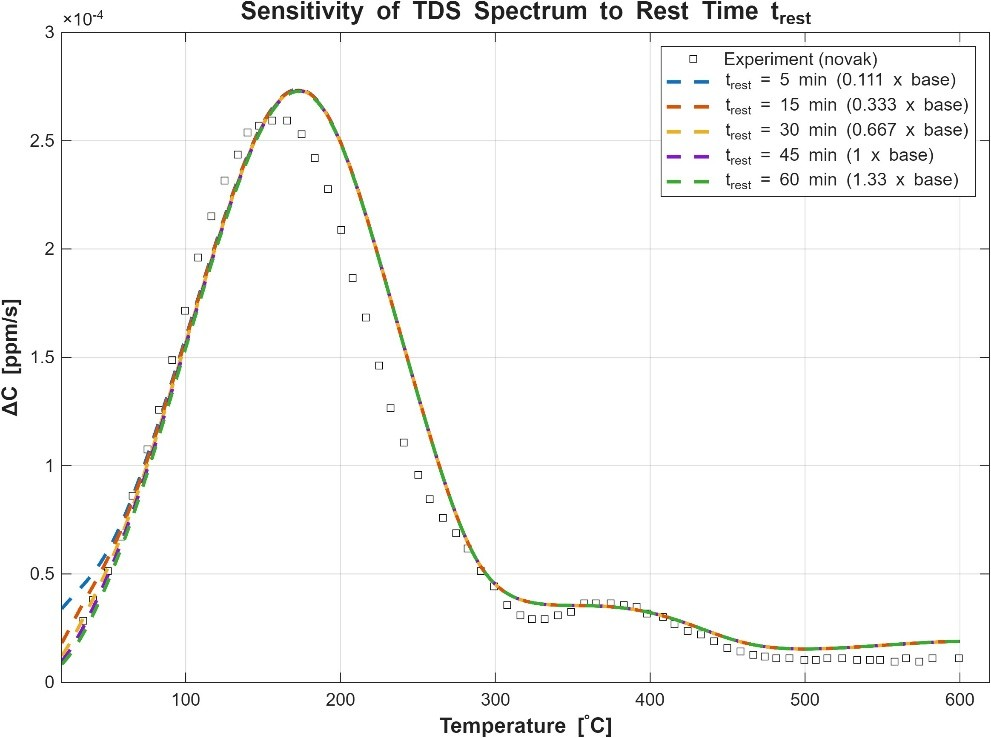
\includegraphics[width=\figwidth]{resttimetds.jpg}
    \caption{Effect of room-temperature rest time on the simulated TDS spectrum.}
    \label{fig:sensitivity_rest_time}
\end{figure}

It can be seen from the TDS curve that there isn't much difference in the TDS spectra except at the starting point of the temperature ramp, where the higher rest times showed a lower flux value at the start of the ramp. The effect of rest time is also of profound importance in thinner samples, where the hydrogen desorption is significantly affected by rest time.

\subsection{Effect of Heating Rate (\texorpdfstring{$\phi$}{phi})}

Heating rate was varied from $50$ to $350\text{ K/h}$ ($0.0139$ to $0.0972\text{ K/s}$).

\begin{figure}[htbp]
    \centering
    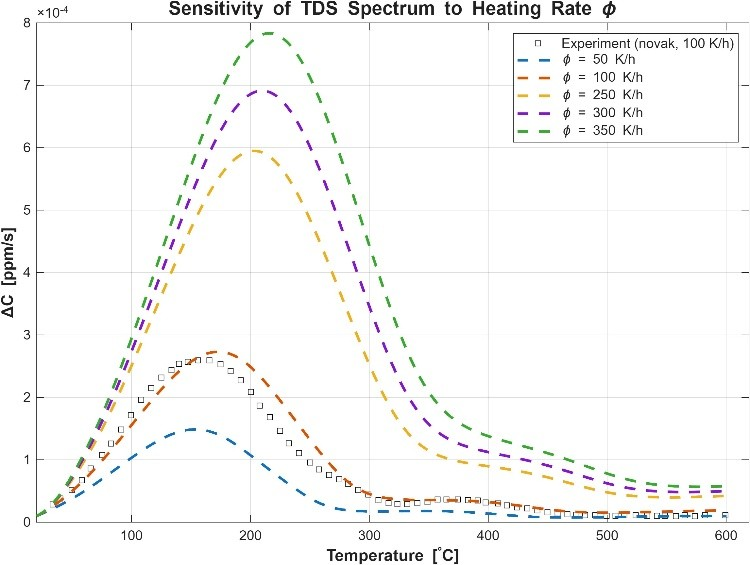
\includegraphics[width=\figwidth]{heatingratetds.jpg}
    \caption{Effect of heating rate on the simulated TDS spectrum.}
    \label{fig:sensitivity_heating_rate}
\end{figure}

\begin{table}[htbp]
\centering
\caption{Effect of Heating Rate}
\label{tab:heating_rate}
\tablestyle
\fitwidth{%
\begin{tabular}{ccccccc}
\toprule
$\phi$ & $J_{\max}$ & $\Delta J_{\max}$ & $T_{\mathrm{p}}$ & $\Delta T_{\mathrm{p}}$ & $H_{\mathrm{des}}$ & \textbf{Spectral} \\
($\text{K/h}$) & ($10^{-4}\text{ ppm/s}$) & ($\%$) & ($^\circ\text{C}$) & ($\text{K}$) & ($\text{ppm}$) & \textbf{Width (\text{K})} \\
\midrule
50         & $1.4865$ & $-45.5\%$  & $153.69$ & $-19.19\text{ K}$ & $1.853$ & $173\text{ K}$ \\
100 (Base) & $2.7299$ & $0.0\%$    & $172.89$ & $0.00\text{ K}$   & $1.831$ & $185\text{ K}$ \\
250        & $5.9497$ & $+117.9\%$ & $203.06$ & $+30.17\text{ K}$ & $1.802$ & $208\text{ K}$ \\
300        & $6.9123$ & $+153.2\%$ & $209.83$ & $+36.94\text{ K}$ & $1.796$ & $215\text{ K}$ \\
350        & $7.8332$ & $+186.9\%$ & $215.81$ & $+42.92\text{ K}$ & $1.791$ & $222\text{ K}$ \\
\bottomrule
\end{tabular}%
}
\end{table}

Desorption flux is mathematically expressed as the product of the release rate per Kelvin ($dC/dT$) and the heating rate ($dT/dt = \phi$):
\begin{equation}
J(t) = \frac{dC}{dt} = \phi \cdot \frac{dC}{dT}
\end{equation}
At higher heating rates, the specimen spends less physical time at any given temperature. Because trapping, detrapping, and lattice diffusion require finite time, hydrogen release is shifted to higher temperatures where kinetic rates are sufficiently fast to match the rapid thermal ramp.

\begin{figure}[htbp]
    \centering
    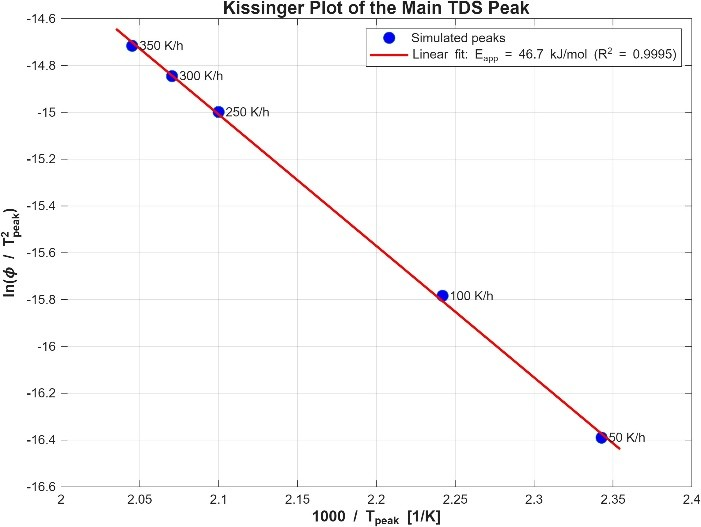
\includegraphics[width=\figwidth]{kissingerplottds.jpg}
    \caption{Kissinger plot from the simulated main peaks, giving an apparent activation energy of $46.7\text{ kJ/mol}$.}
    \label{fig:kissinger_plot}
\end{figure}

Construction of a classic Kissinger plot ($\ln(\phi / T_{\mathrm{p}}^2)$ vs.\ $1/T_{\mathrm{p}}$) across these simulated peak temperatures yields an apparent activation energy of $E_{\mathrm{app}} \approx 47\text{ kJ/mol}$. The true detrapping barrier for Trap 1 is $E_{\mathrm{d,1}} = E_{\mathrm{L}} + |\Delta H_1| = 5.69 + 50.65 = 56.34\text{ kJ/mol}$. We can thus see that the standard Kissinger analysis underestimates the true binding energy by $17\%$ because it neglects internal diffusion resistance and retrapping in thick specimens.

%------------------------------------------------
\section{Experimental Application: X65 Pipeline Steel}
%------------------------------------------------

The McNabb--Foster FEM solver was then applied to our measured experimental data of X65 pipeline steel. The parameters are given in Table~\ref{tab:x65_params}.

\begin{table}[htbp]
\centering
\caption{Master Parameter Summary for X65 Hydrogen Transport Simulation}
\label{tab:x65_params}
\tablestyle
\fitwidth{%
\begin{tabular}{l l c l}
\toprule
\textbf{Category} & \textbf{Parameter Name / Symbol} & \textbf{Value} & \textbf{Unit} \\
\midrule
\textbf{Geometry} & Total Sample Length ($L$) & $0.0005$ & m ($0.5$ mm) \\
& Simulation Domain Length ($L_{\mathrm{domain}}$) & $0.00025$ & m (Symmetric half) \\
& Number of Elements / Nodes ($n_{\mathrm{el}} / n_{\mathrm{node}}$) & $50 / 51$ & -- \\
& Element Length ($h$) & $5 \times 10^{-6}$ & m \\
\midrule
\textbf{Diffusion} & Diffusion Coefficient Prefactor ($D_0$)~\cite{KIUCHI1983961,Marrani2025,Koren2024a} & $7.23 \times 10^{-8}$ & m$^2$/s \\
& Lattice Activation Energy ($E_L$) & $5690$ & J/mol~\cite{KIUCHI1983961,Marrani2025,Koren2024a} \\
& Initial Lattice Concentration ($C_{L,0}$) & $0.555$ & mol/m$^3$ \\
& Jump Frequency ($\nu$) & $1 \times 10^{13}$ & Hz \\
& Converted Lattice Site Density ($N_L$) & $8.47 \times 10^{5}$~\cite{Marrani2025,Krom2000,Fallahmohammadi2013} & mol/m$^3$ ($5.1 \times 10^{29}$ sites/m$^3$) \\
& Universal Gas Constant ($R$) & $8.314$ & J/(mol$\cdot$K) \\
\midrule
\textbf{Test Conditions} & Heating Rate ($\phi$) & $0.0555$ & K/s \\
& Rest Time ($t_{\mathrm{rest}}$) & $1800$ & s \\
& Minimum Temperature ($T_{\min}$) & $301.55$ & K ($28.4$ $^\circ$C) \\
& Maximum Temperature ($T_{\max}$) & $987.55$ & K ($714.4$ $^\circ$C) \\
& Time Step ($\Delta t$) & $0.25$ & s \\
\midrule
\textbf{Boundary} & Surface Penalty Factor ($k_{\mathrm{pen}}$) & $8 \times 10^{6}$ & mol/(m$^2\cdot$s) \\
& Surface Activation Energy ($E_{\mathrm{bc}}$) & $17100$ & J/mol \\
\midrule
\textbf{Trap Kinetics} & Trap 1 ($\Delta H_1, N_{T,1}$) & $-62000, 0.2491$ & J/mol, mol/m$^3$ \\
& Trap 2 ($\Delta H_2, N_{T,2}$) & $-80000, 0.6310$ & J/mol, mol/m$^3$ \\
& Trap 3 ($\Delta H_3, N_{T,3}$) & $-120000, 0.0830$ & J/mol, mol/m$^3$ \\
& Trap 4 ($\Delta H_4, N_{T,4}$) & $-150000, 0.3321$ & J/mol, mol/m$^3$ \\
\bottomrule
\end{tabular}%
}
\end{table}

\begin{figure}[htbp]
    \centering
    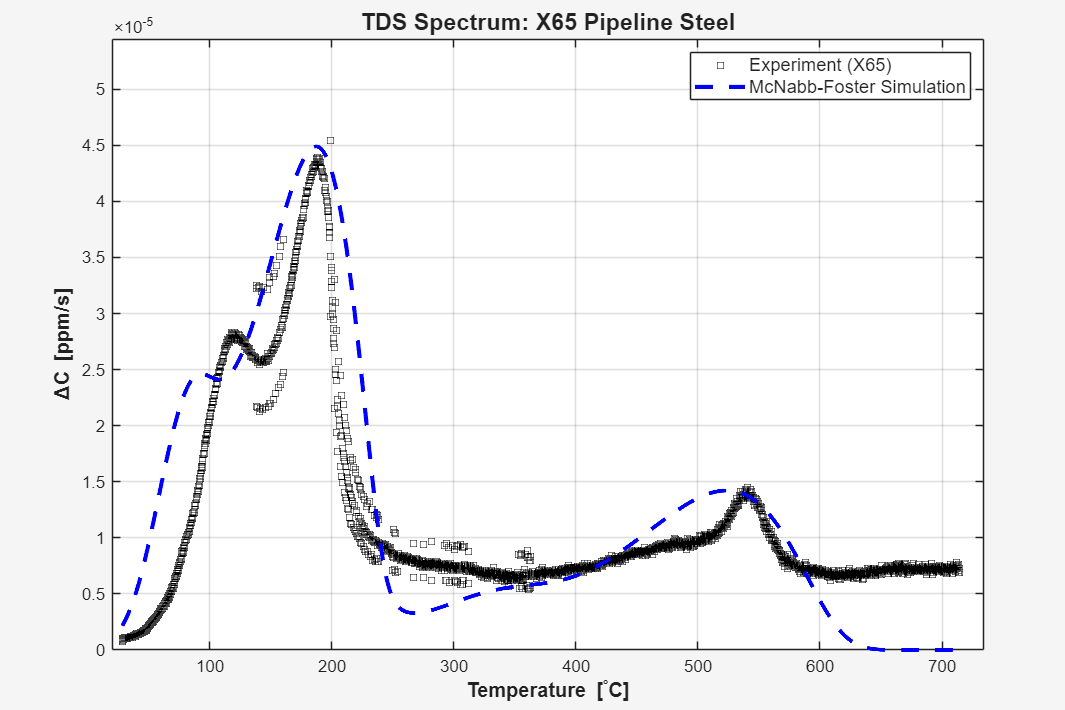
\includegraphics[width=\figwidth]{x65tdsmodified.png}
    \caption{Simulated and experimental TDS spectra for X65 pipeline steel.}
    \label{fig:x65_tds_spectrum}
\end{figure}

\begin{table}[htbp]
\centering
\caption{Comparison of Experimental and Simulated Features for X65 Pipeline Steel}
\label{tab:x65_comparison}
\tablestyle
\begin{tabular}{L{2.4cm} L{3.8cm} L{3.8cm} L{2.9cm}}
\toprule
\textbf{Feature} & \textbf{Experimental Observation (Visual)} & \textbf{Simulated Output (Computed)} & \textbf{Quantitative Difference} \\
\midrule
Low-$T$ Peak & Peak at $\approx 120^\circ\text{C}$, $2.8 \times 10^{-5}\text{ ppm/s}$ & Shoulder at $\approx 90^\circ\text{C}$, $2.4 \times 10^{-5}\text{ ppm/s}$ & $\approx -30\text{ K}$ shift; No resolved peak \\
Main Peak & Peak at $\approx 190^\circ\text{C}$, $4.35 \times 10^{-5}\text{ ppm/s}$ & Peak at $\approx 185^\circ\text{C}$, $4.50 \times 10^{-5}\text{ ppm/s}$ & $\approx -5\text{ K}$ shift; $+3\%$ height \\
High-$T$ Peak & Peak at $\approx 540^\circ\text{C}$, $1.40 \times 10^{-5}\text{ ppm/s}$ & Peak at $\approx 520^\circ\text{C}$, $1.42 \times 10^{-5}\text{ ppm/s}$ & $\approx -20\text{ K}$ shift; $+1\%$ height \\
Mid-$T$ Valley ($250\text{--}350^\circ\text{C}$) & Flux $\approx 0.6\text{--}0.9 \times 10^{-5}\text{ ppm/s}$ & Flux $\approx 0.3\text{--}0.6 \times 10^{-5}\text{ ppm/s}$ & Underestimated desorption flux \\
High-$T$ Plateau ($>620^\circ\text{C}$) & Non-zero plateau $\approx 0.7 \times 10^{-5}\text{ ppm/s}$ & Drops to $0.00\text{ ppm/s}$ above $620^\circ\text{C}$ & Missing high-temperature plateau \\
\bottomrule
\end{tabular}
\end{table}

The model is able to reproduce the overall three-peak structure with the primary peak height matching within $+3\%$ ($4.50$ vs.\ $4.35 \times 10^{-5}\text{ ppm/s}$) and the high-temperature peak height to within $+1\%$ ($1.42$ vs.\ $1.40 \times 10^{-5}\text{ ppm/s}$). There is a thermal offset for the main peak ($5\text{ K}$) that gives a relative error of $\approx 1\%$ on the Kelvin temperature scale ($458\text{ K}$ vs.\ $463\text{ K}$).

The model is unable to resolve the peak at $120^\circ\text{C}$, producing instead an unresolved shoulder at $90^\circ\text{C}$ ($\approx -30\text{ K}$ offset); this may be due to the room-temperature rest loss in a thin specimen. There is an underestimation of flux in the $250\text{--}350^\circ\text{C}$ valley, which suggests a missing intermediate trap state (binding energy between $62$ and $120\text{ kJ/mol}$) or a continuous distribution of trap energies, whereas the peak near $550^\circ\text{C}$ may be due to some artifacts during experiments or hydrogen at higher binding states.

Upon integrating the area of the curve under the experimental curve we get the total hydrogen concentration in the sample as $0.1446\text{ ppm}$ whereas for our simulated curve initial concentration at ($t = 0\text{ s}$) is $0.2376\text{ ppm}$ and with rest time losses the concentration at the start of the TDS experiment is $0.1564\text{ ppm}$ that is it matches with an error of $\approx +8.2\%$. So we can see that in order to get a good match between experimental and simulated TDS concentration there are highly correlated parameters: initial equilibrium concentration, rest time, thickness of the sample, in addition to binding energy and trap density.

\subsection{Thin Specimen Rest Loss}

Because our specimen is very thin ($L = 0.5\text{ mm}$), its pre-heating rest loss behavior differs radically from the $6.3\text{ mm}$ baseline. Pre-heating rest hold hydrogen loss kinetics for X65 steel ($0.5\text{ mm}$) are summarized below. (All values are exact computed solver outputs).

\begin{figure}[htbp]
    \centering
    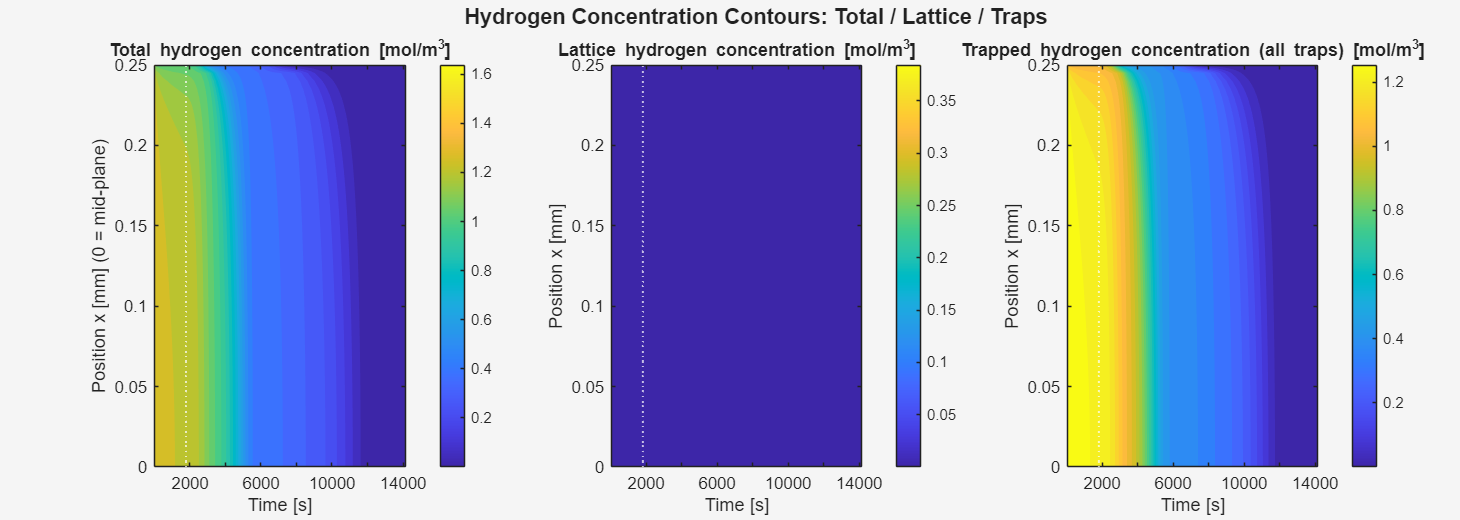
\includegraphics[width=\figwidth]{x65totalconc.png}
    \caption{Total, lattice and trapped hydrogen concentration across the half-thickness of the X65 specimen.}
    \label{fig:x65_concentration_contours}
\end{figure}

\begin{table}[htbp]
\centering
\caption{Rest Time Loss for Thin Specimen ($0.5\text{ mm}$)}
\label{tab:thin_specimen_loss}
\tablestyle
\fitwidth{%
\begin{tabular}{ccc}
\toprule
\textbf{Rest Time $t_{\mathrm{rest}}$ ($\text{s}$)} & \textbf{Mobile Lattice H Change ($\%$)} & \textbf{Total Hydrogen Inventory Change ($\%$)} \\
\midrule
0 s & $0.00\%$ ($4.62 \times 10^{-1}\text{ mol/m}^3$) & $0.00\%$ ($1.76\text{ mol/m}^3$) \\
600 s & $-99.98\%$ ($1.05 \times 10^{-4}\text{ mol/m}^3$) & $-29.68\%$ ($1.24\text{ mol/m}^3$) \\
1200 s & $-99.99\%$ ($6.83 \times 10^{-5}\text{ mol/m}^3$) & $-30.79\%$ ($1.22\text{ mol/m}^3$) \\
1800 s & $-99.99\%$ ($5.27 \times 10^{-5}\text{ mol/m}^3$) & $-31.55\%$ ($1.20\text{ mol/m}^3$) \\
\bottomrule
\end{tabular}%
}
\end{table}

The table shows the effect of rest time for $0.5\text{ mm}$ thickness. Also, from the hydrogen concentration contours, we can see that the lattice hydrogen is almost effectively empty after the rest period in $0.5\text{ mm}$ thin specimens; $> 99.98\%$ of mobile lattice hydrogen desorbs within the first $600\text{ s}$ of rest hold. This rapid surface depletion also creates a severe concentration gradient across the thickness, because of which detrapping also occurs from shallow traps. Consequently, $30\text{ to } 35\%$ of total trapped hydrogen is completely lost prior to heating.

\begin{figure}[htbp]
    \centering
    \begin{subfigure}[b]{0.48\textwidth}
        \centering
        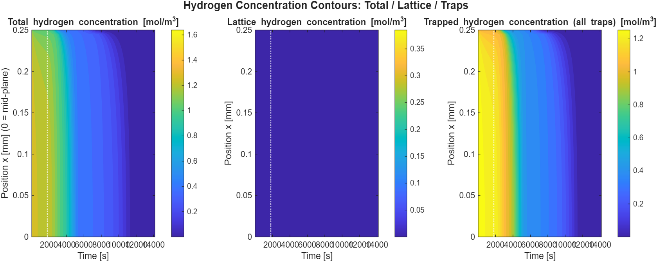
\includegraphics[width=\linewidth]{x65trapconc0point5mm.png}
        \caption{Thickness $L = 0.5\text{ mm}$}
        \label{fig:contour_0p5mm}
    \end{subfigure}\hfill
    \begin{subfigure}[b]{0.48\textwidth}
        \centering
        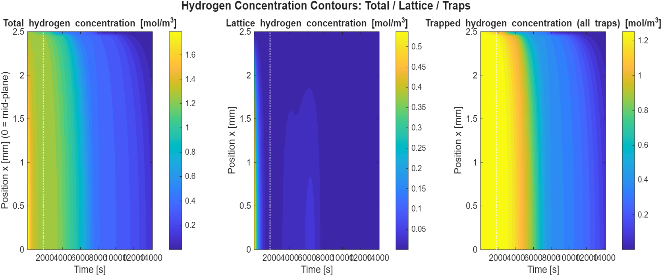
\includegraphics[width=\linewidth]{x65trapconc5mm.png}
        \caption{Thickness $L = 5.0\text{ mm}$}
        \label{fig:contour_5mm}
    \end{subfigure}

    \medskip

    \begin{subfigure}[b]{0.48\textwidth}
        \centering
        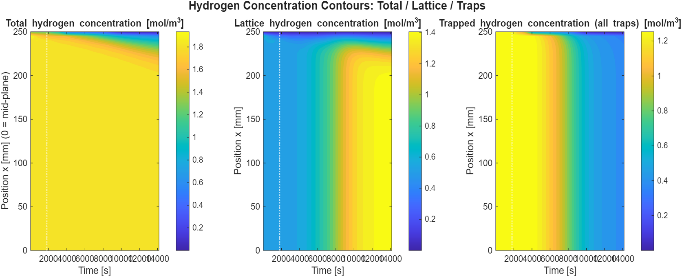
\includegraphics[width=\linewidth]{x65trapconc50mm.png}
        \caption{Thickness $L = 50.0\text{ mm}$}
        \label{fig:contour_50mm}
    \end{subfigure}\hfill
    \begin{subfigure}[b]{0.48\textwidth}
        \centering
        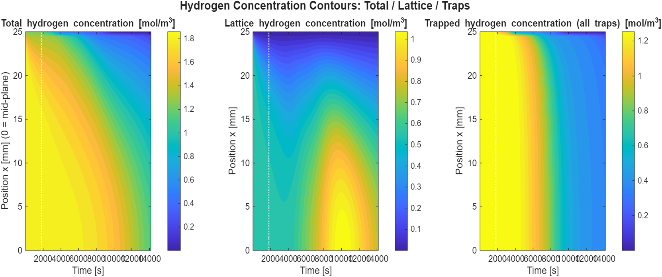
\includegraphics[width=\linewidth]{x65trapconc500mm.png}
        \caption{Thickness $L = 500.0\text{ mm}$}
        \label{fig:contour_500mm}
    \end{subfigure}
    \caption{Hydrogen concentration contours for specimen thicknesses from $0.5\text{ mm}$ to $500\text{ mm}$.}
    \label{fig:thickness_contours_grid}
\end{figure}

If we keep the rest time constant and vary the thickness, we see that for thick specimens ($50\text{--}500\text{ mm}$), the interior hydrogen remains completely shielded (loss $< 5\%$). So for a thin specimen, particularly in this case, the lower temperature peak can be significantly affected by uncertainties in exact rest time measurement.

\subsection{Summary of Key Findings}

Trial and error trap parameters gave reasonable agreement with the experimental curve. However, it should be noted that the system is highly ill-posed; that is, multiple combinations of binding energy and trap density can give the same TDS spectra, thus further pushing the need for a machine learning (ML) model to address this issue. The thickness of the sample is also a crucial factor for our study as it can effectively reduce the amount of hydrogen that is desorbed, thus changing the TDS spectra. The aim of this study was to establish that, given a sensible range for binding energy and trap density, we can approximately reproduce the TDS curve for one particular combination. The values of parameters might represent one particular set of solutions, but detailed analysis is further required.

%================================================
% CHAPTER 5
%================================================
\chapter{Inverse Problem and Machine-Learning Framework}
\label{ch:inverse}

\section{Forward and Inverse Problems}
\label{sec:fwd-inv}

The FEM model developed in this work represents the forward problem. Given a set of material, trap, specimen, and experimental parameters, the model calculates the corresponding TDS response:
\begin{equation}
  \boldsymbol{\theta} \;\longrightarrow\; \text{FEM} \;\longrightarrow\; J_{\mathrm{des}}(T).
  \label{eq:forward}
\end{equation}
Here,
\begin{equation}
  \boldsymbol{\theta} = \left[ D_0,\, E_L,\, E_b^{(1)},\dots,E_b^{(n_t)},\,
  N_T^{(1)},\dots,N_T^{(n_t)},\, C_{L,0},\, L_d,\, \beta,\, t_{\mathrm{rest}},\, \dots \right].
  \label{eq:theta}
\end{equation}
Note that in this chapter $\boldsymbol{\theta}$ denotes the parameter vector and should not be confused with the occupancies $\theta_L$ and $\theta_T$ used in Chapter~\ref{ch:formulation}.

The inverse problem is the reverse mapping,
\begin{equation}
  J_{\mathrm{des}}(T) \;\longrightarrow\; \text{ML} \;\longrightarrow\; \hat{\boldsymbol{\theta}}.
  \label{eq:inverse}
\end{equation}

\section{Synthetic Dataset}
\label{sec:dataset}

The objective of the subsequent phase is to learn this inverse relationship from synthetic data generated by the verified forward model. It is therefore proposed to generate a large synthetic dataset using the physically meaningful parameters of the FEM model. Each simulation will produce a complete temperature-dependent desorption response together with the parameter vector used to generate it. A generic dataset entry can therefore be represented as
\begin{equation}
  \left\{ T_j,\; J_{\mathrm{des}}(T_j),\; \boldsymbol{\theta} \right\}.
  \label{eq:entry}
\end{equation}

\section{Prediction Tasks}
\label{sec:tasks}

The proposed inverse model may contain multiple prediction tasks. The first task is classification of the number of trap populations,
\begin{equation}
  \hat{n}_t = f_{\mathrm{cls}}\!\left(J_{\mathrm{des}}\right).
  \label{eq:cls}
\end{equation}
The second task is regression of trap binding energies,
\begin{equation}
  \hat{E}_b = f_E\!\left(J_{\mathrm{des}}\right),
  \label{eq:regE}
\end{equation}
and the third is regression of trap densities,
\begin{equation}
  \hat{N}_T = f_N\!\left(J_{\mathrm{des}}\right).
  \label{eq:regN}
\end{equation}

\section{Input Representations}
\label{sec:inputs}

In the literature, two approaches are used~\cite{Marrani2025,Yang2025}; however, they need to be studied further. The first approach uses the complete normalised TDS curve as the input. The curve can be normalised either by its area or by its peak value. In this representation,
\begin{equation}
  \mathbf{x} = \left[ J_{\mathrm{des}}(T_1),\, J_{\mathrm{des}}(T_2),\, \dots,\, J_{\mathrm{des}}(T_m) \right].
  \label{eq:xfull}
\end{equation}
The second approach uses physically meaningful extracted features, such as
\begin{equation}
  \mathbf{x}_{\mathrm{feat}} = \left[ J_{\max},\, T_{\mathrm{peak}},\, W_{\mathrm{peak}},\,
  H_{\mathrm{des}},\, \text{shoulder descriptors},\, \dots \right],
  \label{eq:xfeat}
\end{equation}
where $J_{\max}$ is the maximum desorption flux, $T_{\mathrm{peak}}$ is the peak temperature, $W_{\mathrm{peak}}$ is the peak width, and $H_{\mathrm{des}}$ is the total desorbed hydrogen.

A possible framework is a neural network that is capable of this classification and regression.

\section{Proposed End-to-End Workflow}
\label{sec:workflow}

The FEM model is therefore not merely a data generator. It defines the physical assumptions under which the machine-learning inverse mapping is learned.

%================================================
% CHAPTER 6
%================================================
\chapter{Current Status and Future Work}
\label{ch:status}

\section{Work Completed in Phase I}
\label{sec:phase1}

The principal work completed during Phase I can be summarised as follows:
\begin{enumerate}
  \item A literature review of hydrogen diffusion, trapping, TDS, and numerical hydrogen transport models was completed.
  \item The distinction between Oriani local-equilibrium trapping and McNabb--Foster transient kinetic trapping was established.
  \item A one-dimensional transient multi-trap hydrogen transport model was formulated.
  \item The model was implemented using the finite-element method in MATLAB.
  \item Four discrete trap populations were incorporated into the transient kinetic formulation.
  \item Initial trap populations were established using an Oriani equilibrium partition at the initial temperature.
  \item A temperature-programmed desorption calculation was implemented.
  \item Mesh and time-step independence studies were performed.
  \item Sensitivity studies were conducted for trap binding energy, trap density, initial hydrogen concentration, lattice diffusion parameters, surface penalty parameters, specimen thickness, rest time, and heating rate.
  \item A preliminary comparison with an experimental X65 TDS response was performed using an approximate four-trap parameter set.
  \item The results demonstrated that the FEM framework captures physically interpretable relationships between hydrogen transport, trapping, and thermal desorption.
\end{enumerate}

\section{Limitations of the Current Phase}
\label{sec:limitations}

However, there are several limitations of the current phase, such as uncertainty regarding several parameters, like the initial concentration and the varying diffusion coefficient, and not knowing the proper number of traps. These uncertainties need to be studied and properly quantified in the next phase.

%================================================
% CHAPTER 7
%================================================
\chapter{Conclusion}
\label{ch:conclusion}

The present Phase~I work established a physics-based finite-element framework for transient hydrogen diffusion, trapping, detrapping, and thermal desorption in a one-dimensional ferritic pipeline-steel specimen.

The model uses a McNabb--Foster transient kinetic formulation in which lattice hydrogen diffuses through the material while multiple trap populations exchange hydrogen with the mobile lattice. The initial hydrogen partition is set up using an Oriani equilibrium relation, after which the transient heating simulation is governed by finite trapping and detrapping kinetics.

A numerical mesh and time-step study was carried out, and an appropriate mesh and time step were found that do not cause changes in the numerical simulations. A baseline simulation was performed to check that our numerical model is capable of reproducing literature-verified TDS curves. Sensitivity studies were carried out, and then preliminary four-trap simulations of X65 pipeline steel were performed using approximately calibrated values of binding energy and trap density,
\begin{multline}
  \left(E_b^{(i)},\, N_T^{(i)}\right) = \\
  \left[ (62,\, 1.5\times10^{23}),\; (80,\, 3.8\times10^{23}),\;
         (120,\, 0.5\times10^{23}),\; (150,\, 2.0\times10^{23}) \right],
  \label{eq:fourtrap}
\end{multline}
with energies in $\mathrm{kJ\,mol^{-1}}$ and densities in $\mathrm{sites\,m^{-3}}$. (In the code, $N_T^{(i)}$ is converted to $\mathrm{mol\,m^{-3}}$ by dividing by Avogadro's number, $6.022\times10^{23}\,\mathrm{mol^{-1}}$; for example, $1.5\times10^{23}\,\mathrm{sites\,m^{-3}}\approx 0.25\,\mathrm{mol\,m^{-3}}$.) These values provide a useful initial computational representation. However, they remain preliminary and should not be interpreted as a unique experimental identification.

The Phase~I results therefore establish the forward FEM framework required for the next stage of the research. The central remaining problem is the inverse mapping from measured TDS response to hydrogen trap parameters. Because the sensitivity studies demonstrate parameter coupling and potential non-uniqueness, this inverse problem requires a controlled synthetic dataset, physically justified experimental conditions, and systematic validation.

The subsequent phase will therefore focus on refinement of the hydrogen charging boundary condition, systematic parameter identifiability analysis, generation of a physics-based synthetic TDS database, and development of a machine-learning framework for inverse identification of hydrogen trap parameters. The final objective is not simply to reproduce an experimental TDS curve, but to establish a physics-informed computational framework in which the inferred trap parameters can be evaluated for physical consistency and uniqueness.

%================================================
% REFERENCES
%================================================
\clearpage
\phantomsection
\addcontentsline{toc}{chapter}{References}
\begin{singlespace}
\bibliographystyle{unsrt}
\bibliography{mybib}
\end{singlespace}

\end{document}